% Overleaf settings:
% compiler: XeLaTeX

\documentclass[type=doctor,fontset=custom,pifootnote]{thuthesis}
% 选项:
%   type=[bachelor|master|doctor|postdoctor], % 必选
%   fontset=[fandol|custom],                  % 字体选择
%   secret,                                   % 可选
%   pifootnote,                               % 可选(建议打开)
%   openany|openright,                        % 可选,基本不用
%   arial,                                    % 可选,基本不用
%   arialtoc,                                 % 可选,基本不用
%   arialtitle                                % 可选,基本不用

% **生僻字乱码的解决方法**
% 先解释一下原因: 自带的 fandol 字体不包含生僻字,常用的中易字体因为版权
% 原因不能在 overleaf 发布。
% 解决方法: 找一台 windows 电脑,从 C:\Windows\Fonts 里把
%   simsun.ttc simhei.ttf simkai.ttf simhei.ttf
% 复制出来,上传到 fonts 文件夹,再设置 typeset=custom 即可。


% 所有其它可能用到的包都统一放到这里了,可以根据自己的实际添加或者删除。
\usepackage{thuthesis}

% 定义所有的图片文件在 figures 子目录下
\graphicspath{{figures/}}

% 可以在这里修改配置文件中的定义。导言区可以使用中文。
% \def\myname{文豪}

\usepackage{xeCJKfntef}

\usepackage{amsmath,amsfonts,mathrsfs}

\usepackage{tikz-cd}
\usepackage{tikz}
\usetikzlibrary{trees,arrows,external}
% \tikzexternalize[prefix=tikz/]


\usepackage[all]{xy}
\usepackage{xcolor}
\usepackage{cases}
\usepackage{dashbox}

\usepackage{pst-func}

\usepackage{MnSymbol}

\newcommand{\qcohsheaf}{^{\mbox{$\sim$}}}
\DeclareMathOperator{\support}{Supp}
\DeclareMathOperator{\coker}{coker}
\DeclareMathOperator{\realpart}{\mathfrak{Re}}
\DeclareMathOperator{\imaginarypart}{\mathfrak{Im}}
\DeclareMathOperator{\gaga}{an}
\DeclareMathOperator{\aut}{Aut}
\DeclareMathOperator{\gl}{GL}
\DeclareMathOperator{\codim}{codim}
\DeclareMathOperator{\gal}{Gal}
\DeclareMathOperator{\diag}{diag}
\newcommand{\resp}{\textit{resp}.\xspace}
\newcommand{\intersect}{\cdot\ldots\cdot}
\DeclareMathOperator{\ann}{Ann}
\DeclareMathOperator{\res}{Res}
\DeclareMathOperator{\proj}{Proj}
\DeclareMathOperator{\PROJ}{\mathbf{Proj}}
\DeclareMathOperator{\car}{car}
\DeclareMathOperator{\Bs}{Bs}
\DeclareMathOperator{\Lb}{B}
\DeclareMathOperator{\des}{des}
\DeclareMathOperator{\sudeg}{\mathrm{su}\widehat{\deg}_{\mathrm{n}}}
\DeclareMathOperator{\udeg}{\mathrm{u}\widehat{\deg}_{\mathrm{n}}}
\DeclareMathOperator{\ndeg}{\widehat{\deg}_{\mathrm{n}}}
\DeclareMathOperator{\Hom}{Hom}
\DeclareMathOperator{\sheafhom}{\mathcal{H}om}
\DeclareMathOperator{\identity}{Id}
\DeclareMathOperator{\Image}{Im}
\DeclareMathOperator{\Pic}{Pic}
\DeclareMathOperator{\pr}{pr}
\DeclareMathOperator{\rg}{rg}
\DeclareMathOperator{\reg}{\mathrm{reg}}
\DeclareMathOperator{\sgn}{sgn}
\DeclareMathOperator{\sing}{\mathrm{sing}}
\DeclareMathOperator{\spec}{Spec}
\DeclareMathOperator{\SPEC}{\mathbf{Spec}}
\DeclareMathOperator{\tr}{Tr}
\DeclareMathOperator{\ord}{ord}
\newcommand{\wmu}{\widehat{\mu}}
\newcommand{\uomega}{\overline{\omega}}
\newcommand{\adeg}{\widehat{\deg}}
\DeclareMathOperator{\sym}{Sym}
\newcommand{\ndot}{\raisebox{.4ex}{.}}

\allowdisplaybreaks


\begin{document}

%%% 封面部分
\frontmatter
\thusetup{
  %******************************
  % 注意:
  %   1. 配置里面不要出现空行
  %   2. 不需要的配置信息可以删除
  %******************************
  %
  %=====
  % 秘级
  %=====
%   secretlevel={秘密},
%   secretyear={10},
  %
  %=========
  % 中文信息
  %=========
  ctitle={定义在数域上的超曲面的\\重数计数问题},
  cdegree={理学博士},
  cdepartment={数学科学系},
  cmajor={数学},
  cauthor={文豪},
  csupervisor={张贺春教授},
%   cassosupervisor={陈文光教授}, % 副指导老师
%   ccosupervisor={某某某教授}, % 联合指导老师
  % 日期自动使用当前时间,若需指定按如下方式修改:
  cdate={二〇一七年十二月},
  %
  % 博士后专有部分
%   cfirstdiscipline={计算机科学与技术},
%   cseconddiscipline={系统结构},
%   postdoctordate={2009年7月——2011年7月},
%   id={编号}, % 可以留空: id={},
%   udc={UDC}, % 可以留空
%   catalognumber={分类号}, % 可以留空
  %
  %=========
  % 英文信息
  %=========
  etitle={Counting Multiplicities in a Hypersurface over Number Fields},
  % 这块比较复杂,需要分情况讨论:
  % 1. 学术型硕士
  %    edegree:必须为Master of Arts或Master of Science(注意大小写)
  %             “哲学、文学、历史学、法学、教育学、艺术学门类,公共管理学科
  %              填写Master of Arts,其它填写Master of Science”
  %    emajor:“获得一级学科授权的学科填写一级学科名称,其它填写二级学科名称”
  % 2. 专业型硕士
  %    edegree:“填写专业学位英文名称全称”
  %    emajor:“工程硕士填写工程领域,其它专业学位不填写此项”
  % 3. 学术型博士
  %    edegree:Doctor of Philosophy(注意大小写)
  %    emajor:“获得一级学科授权的学科填写一级学科名称,其它填写二级学科名称”
  % 4. 专业型博士
  %    edegree:“填写专业学位英文名称全称”
  %    emajor:不填写此项
  edegree={Doctor of Philosophy},
  emajor={Mathematics},
  eauthor={Wen Hao},
  esupervisor={Professor Zhang Hechun},
%   eassosupervisor={Chen Wenguang},
  % 日期自动生成,若需指定按如下方式修改:
  edate={December, 2017}
  %
  % 关键词用“英文逗号”分割
  ckeywords={重数计数, 射影超曲面, 高度函数, 一般化的 Schanuel 估计, 相交树},
  ekeywords={counting multiplicity, projective hypersurface, height function, generalized Schanuel's estimate, intersection tree}
}

% 定义中英文摘要和关键字
\begin{cabstract}
考虑定义在数域上的射影超曲面,我们可以通过局部 Hilbert-Samuel 函数定义其上点的重数。取定一个计数函数,我们考虑在这个射影超曲面上代数点的重数的计数问题:即对超曲面上,高度不超过定值,定义域相对于基域的扩张次数等于一个定值的所有代数点,用取定的计数函数作用在这些点的重数上,求和。本文将对这个问题给出一个上界估计,这个上界将会与射影超曲面的次数,奇点集的维数,高度的上界,以及相应域扩张次数有关。这个估计可以在某种程度上衡量射影超曲面的奇点集的复杂程度。
\end{cabstract}

% 如果习惯关键字跟在摘要文字后面,可以用直接命令来设置,如下:
% \ckeywords{\TeX, \LaTeX, CJK, 模板, 论文}

\begin{eabstract}
We fix a counting function of multiplicities of algebraic points in a projective hypersurface over a number field, and take the sum over all algebraic points of bounded height and fixed degree. An upper bound for the sum with respect to this counting function will be given in terms of the degree of the hypersurface, the dimension of the singular locus, the upper bounds of height, and the degree of the field of definition. This upper bound gives a description of the complexity of the singular locus of this hypersurface to some extent.
\end{eabstract}

% \ekeywords{\TeX, \LaTeX, CJK, template, thesis}

% 如果使用授权说明扫描页,将可选参数中指定为扫描得到的 PDF 文件名,例如:
% \makecover[scan-auth.pdf]
\makecover

%% 目录
\tableofcontents

%% 符号对照表
\begin{denotation}[3cm]
\item[$\mathbb{N}$] 自然数集
\item[$\mathbb{Z}$] 有理整数环
\item[$\mathbb{Q}$] 有理数域
\item[$\mathbb{R}$] 实数数域
\item[$\mathbb{C}$] 复数数域
\item[$\mathbb{F}_q$] 元素个数等于$q$的有限域
\item[$\operatorname{ht}(\mathfrak{a})$] 环的理想$\mathfrak{a}$的高度
\item[$\ann_A(M)$] $A$-模$M$的零化理想
\item[$\support(M)$] $A$-模$M$的支集
\item[$\operatorname{depth}(M)$] Noetherian 局部环上的模$M$的深度
\item[$\ell_A(M)$] $A$-模$M$的长度
\item[$\chi_M(\cdot)$] $A$-模$M$的 Hilbert-Samuel 函数
\item[$e_{\mathfrak{q},M}$] $A$-模$M$关于理想$\mathfrak{q}$的重数
\item[$e_{M}$] 局部环$A$上的模$M$的重数
\item[$e_{A}$] 局部环$A$的重数
\item[$\spec(A)$] 环$A$的素谱
\item[$\operatorname{Frac}(A)$] 整环$A$的分式域
\item[$K(A)$] 环$A$的全商环
\item[$K(X)$] 整概型$X$的函数域
\item[$\mathbb{A}_K^n$] 数域$K$上的$n$维仿射空间
\item[$\mathbb{P}_K^n$] 数域$K$上的$n$维射影空间
\item[$\sym$] 对称代数
\item[$\SPEC(\mathscr{F})$] 代数层$\mathscr{F}$的素谱
\item[$\PROJ(\mathscr{F})$] 分次代数层$\mathscr{F}$相伴的射影概型
\item[$\mathbb{P}(\mathscr{E})$] 向量丛$\mathscr{E}$相伴的射影空间丛
\item[$H_{\xi}(\cdot)$] 射影概型$X$在点$\xi$处的局部 Hilbert-Samuel 函数
\item[$\mu_{\xi}(X)$] 点$\xi$在射影概型$X$里的重数
\item[$\mu_M(X)$] 整闭子概型$M$在射影概型$X$里的重数
\item[$\mathcal{O}_K$] 数域$K$的整数环
\item[$N(\mathfrak{a})$] 环的理想$\mathfrak{a}$的范数
\item[$h_K$] 数域$K$的类数
\item[$R_K$] 数域$K$的调控子(又称导子)
\item[$\omega_K$] 数域$K$中单位根个数
\item[$\Delta_K$] 数域$K$的判别式
\item[$M_K$] 数域$K$的所有位点之集
\item[$M_{K,f}$] 数域$K$的所有有限位点之集
\item[$M_{K,\infty}$] 数域$K$的所有无限位点之集
\item[$\ord_v$] 数域$K$在有限位点$v$的$v$-进赋值
\item[$|a|_v$] 数域$K$中元素$a$的$v$-进绝对值
\item[$\|a\|_v$] 数域$K$中元素$a$的规范化的$v$-进绝对值
\item[$K_v$] 数域$K$在位点$v$处完备化得到的局部域
\item[$\mathcal{O}_{v}$] 局部域$K_v$的整数环
\item[$\mathbb{C}_v$] 局部域$K_v$取代数闭包再取完备化得到的域
\item[$\mathbb{A}_K$] 数域$K$的加元环(ad\`{e}le ring)
\item[$\mathbb{A}_K^\times$] 数域$K$的理元群(id\`{e}le group)
\item[$e(\mathfrak{P}|\mathfrak{p})$] 代数整数环的扩张中,扩环的素理想$\mathfrak{P}$关于整除它的基环的素理想$\mathfrak{p}$的分歧指数
\item[$f(\mathfrak{P}|\mathfrak{p})$] 代数整数环的扩张中,扩环的素理想$\mathfrak{P}$关于整除它的基环的素理想$\mathfrak{p}$的剩余次数
\item[$\|x\|_v$] $\mathbb{C}_v$-线性空间中向量$x$的范数
\item[$\zeta_K(\cdot)$] 数域$K$的$\zeta$函数
% \item[$\[E:K\]$] 域扩张$K\subseteq E$的次数
\item[$\gal(E/K)$] 域的Galois扩张$K\subseteq E$的 Galois 群
\item[$N_{E/K}(\cdot)$] 域扩张$K\subseteq E$的范
\item[$\tr_{E/K}(\cdot)$] 域扩张$K\subseteq E$的迹
\item[$K(\xi)$] 射影空间中点$\xi$的定义域
\item[$H_K(\cdot)$] 射影空间上相对数域$K$的乘性高度函数
\item[$h(\cdot)$] 射影空间上的绝对对数高度函数
\item[$h_{\phi}(\cdot)$] 射影概型$X$上关于闭浸入$\phi: X \to \mathbb{P}_K^n$的绝对对数高度函数
\item[$\mathcal{O}(1)$] 射影空间上的 Serre 扭层,泛线丛
\item[$\mathscr{L}(D)$] 与射影概型上 Cartier 除子$D$相伴的线丛
\item[$\operatorname{Div}(X)$] 与射影概型上 Cartier 除子群
\item[$\operatorname{CaCl}(X)$] 射影概型$X$的 Cartier 除子类群
\item[$\Pic(X)$] 射影概型$X$的 Picard 群
\item[$E^{\vee}$] 向量丛$E$的对偶
\item[$\det(E)$] 向量丛$E$的行列式丛
% \item[$\widehat{\deg}(\overline{E})$] Hermitian 向量丛$\overline{E}$的 Arakelov 高度
% \item[$\widehat{\deg}_n(\overline{E})$] Hermitian 向量丛$\overline{E}$的规范化的 Arakelov 高度
% \item[$h_{\overline{\mathscr{L}}}(\cdot)$] 代数整数环上的平坦射影概型上的相对 Hermitian 线丛$\overline{\mathscr{L}}$的 Arakelov 高度函数
\item[$H_{\widetilde{\mathscr{L}}, K}(\cdot)$] 数域$K$上的光滑射影簇上关于 Adelic 线丛$\widetilde{\mathscr{L}}$相对于数域$K$的高度函数
\item[$H_{\widetilde{\mathscr{L}}}(\cdot)$] 数域$K$上的光滑射影簇上关于 Adelic 线丛$\widetilde{\mathscr{L}}$的绝对高度函数
\item[$\mathscr{C}_X$] 概型$X$上的连续函数层
\item[$X^{\mathrm{sing}}$] 概型$X$的奇点集
\item[$X^{\mathrm{reg}}$] 概型$X$的正则点集
\item[$S(X;D,B)$] 数域上的射影概型$X$上高度不超过B且定义域相对基域扩张次数等于$D$的代数点的集合
\item[$S(X;B)$] 数域上的射影概型$X$上高度不超过B的有理点的集合
\item[$N(X;D,B)$] 集合$S(X;D,B)$的势
\item[$N(X;B)$] 集合$S(X;B)$的势
\item[$X_1\intersect X_r$] 正则射影概型的闭子概型$X_1,\cdots,X_r$的相交积
\item[$i(M;X_1\intersect X_r)$] 相交积$X_1\intersect X_r$在不可约分支$M$处的相交重数
\item[$w_{\mathscr{T}}(\ell)$] 相交树$\mathscr{T}$的边$\ell$的权重
\item[$w_{\mathscr{T}}(X)$] 相交树$\mathscr{T}$的顶点$X$的权重
\item[$W_{\mathscr{T}}(Z)$] 基概型的闭子概型$Z$在相交树$\mathscr{T}$中的权重
\end{denotation}



%%% 正文部分
\mainmatter
\chapter{引论}
\label{introduction}

\section{问题的引入}
\label{history}

在本篇论文中,我们将考虑射影概型上代数点(或更简单一些,有理点)的重数计数的问题。具体来说,设$k$为一个域,$X$为$\spec k$上的一个射影概型,考虑以下形式和的估计
\begin{equation}
\sum_{\xi \in S(X(\overline{k}))} f\left(\mu_{\xi}(X)\right),
\end{equation}
其中$S(X(\overline{k}))$是$X(\overline{k})$的满足某些条件(具体的条件在以后的章节中会明确地给出)的子集;$f$是一个把正整数集映射到非负整数集的增函数,我们称其为计数函数;$\mu_{\xi}(X)$是点$\xi$在射影概型$X$里的重数。此重数是由射影概型$X$在点$\xi$处的局部 Hilbert-Samuel 函数给出的,其定义可以简述如下,更多更详细的内容将在随后的章节\ref{chapter:multiplicity}中给出。

我们称 Noether 概型$X$是一个维数纯的概型(或称$X$有纯的维数),如果$X$所有的不可约分支有相同的维数。设$X$是一个维数纯的概型,$\xi \in X$为一个点。我们考虑局部环$\mathcal{O}_{X,\xi}$,并记它的极大理想为$\mathfrak{m}_{\xi}$,剩余类域为$\kappa(\xi)$。我们定义概型$X$在点$\xi$处的局部 Hilbert-Samuel 函数为
\begin{equation}
H_{\xi}(m) = \dim_{\kappa(\xi)} \left(\mathfrak{m}_{\xi}^m/\mathfrak{m}_{\xi}^{m+1}\right),
\end{equation}
其中$m \in \mathbb{N}^+$。设$\dim(\mathcal{O}_{X,\xi}) = t \geqslant 1$,那么存在次数等于$t-1$的多项式$P_{\xi}(T)$使得当$m$充分大时,有$H_{\xi}(m) = P_{\xi}(m)$。更进一步,多项式$P_{\xi}(m)$可以写为
\begin{equation} \label{local Hilbert-Samuel}
P_{\xi}(m) = \mu_{\xi}(X) \frac{m^{t-1}}{(t-1)!} + o(m^{t-1}),
\end{equation}
其中$\mu_\xi(X)$是一个正整数。我们定义$\mu_\xi(X)$为点$\xi$在概型$X$里的重数。若$\dim(\mathcal{O}_{X,\xi}) = 0$,那么$\mathcal{O}_{X,\xi}$是一个局部 Artin 环,此时点$\xi$在概型$X$中的重数$\mu_{\xi}(X)$被定义作这个局部 Artin 环的长度。特别地,如果点$\xi$在$X$上是正则的,即$\mathcal{O}_{X,\xi}$是一个正则局部环,那么我们有$\mu_{\xi}(X) = 1.$

若我们把计数函数$f$取为取值恒为$1$的常值函数,那么我们的问题就简化为了概型$X$的代数点,或者有理点计数这个经典的问题。迄今为止,这个问题已经有许多人做过了大量的研究,成果非常丰富。目前这个领域的研究也仍然是很活跃的。本文问题的研究,也需要大量地利用到关于这个经典问题的前人的成果。

如果我们要求计数函数$f$非平凡,并且还满足$f(1) = 0$,那么这个问题就变成了一个关于概型$X$的奇点集的复杂度的问题。而事实上,本文在研究数域上射影超曲面上重数计数问题所采用的计数函数就是满足这一条件的函数。


\section{已有的一些结果}
设$X$是一个次数为$\delta$的既约的射影平面曲线,我们有
\begin{equation} \label{intro-fulton-multiplicity}
\sum\limits_{\xi\in X} \mu_{\xi}(X) \left(\mu_{\xi}(X)-1\right) \leqslant \delta(\delta-1).
\end{equation}
关于这个结果,具体可参阅参考文献~\inlinecite{Fulton2}第115页的习题5-22。证明的方法主要运用了相交理论中的 B\'ezout 定理。更进一步,设$g(X)$是曲线$X$的亏格,如果$X$是几何整的,那么我们有
\begin{equation}
g(X) \leqslant \dfrac{(\delta-1)(\delta-2)}{2} - \sum_{\xi \in X} \dfrac{\mu_{\xi}(X)\left(\mu_{\xi}(X)-1\right)}{2}.
\end{equation}
具体可以参阅参考文献~\inlinecite{Fulton2}201页的 Corollary 1。这是平面曲线的 Riemann-Roch 定理的一个推论。

更一般地,令$X \hookrightarrow \mathbb{P}^n_k$为定义在一个代数闭的特征等于$0$的域$k$上的射影超曲面,并假设它的奇点集$X^{\mathrm{sing}}$的维数等于$0$。参考文献~\inlinecite{Laumon1975}的 Corollaire 4.2.1 的一个直接推论为
\begin{equation}
\sum_{\xi\in X} \mu_\xi(X)(\mu_{\xi}(X)-1)^{n-1} \leqslant \delta(\delta-1)^{n-1}.
\end{equation}
文献~\inlinecite{Laumon1975}的作者主要使用了Lefschetz束的方法。但是,这些结论有一定的局限性,例如奇点集维数为0这个条件,对于一个一般的计数问题来说,就太严格了。而且,一般地,以上不等式左边的求和是和基域$k$的选取有关的。

一个比较新的结果是,在文章~\inlinecite{Liu-multiplicity}中(Th\'eor\`eme 5.1),刘春晖得到了有限域上的此类的结论。具体来讲,令$X \hookrightarrow \mathbb{P}^n_{\mathbb{F}_q}$为一个既约的射影超曲面,其中$\mathbb{F}_q$是元素个数等于$q$的有限域,$q$为某个素数的幂。设超曲面$X$的奇点集$X^{\mathrm{sing}}$的维数等于$s$,他证明了
\begin{equation} \label{Liu equality}
\sum_{\xi\in X(\mathbb{F}_q)} \mu_{\xi}(X)(\mu_\xi(X)-1)^{n-s-1}\ll_n\delta^{n-s}\max\{\delta-1,q\}^{s}.
\end{equation}
上式中的Vinogradov符号$\ll$具体定义如下:设$\Omega$和$P$为两个集合,$\widetilde{\Omega}$为$\Omega\times P$的一个子集。假设$f(x,y)$和$g(x,y)$定义在集合$\widetilde{\Omega}$上的实值函数,其中$x\in\Omega$,$y\in P$,那么记号
\begin{equation}
f(x,y) \ll_{y} g(x,y)
\end{equation}
指的是,存在定义在集合$P$上的非负函数$C(\ndot)$,对任意的$(x,y) \in \widetilde{\Omega}$满足如下不等式
\begin{equation}
|f(x,y)| \leqslant C(y)|g(x,y)|.
\end{equation}
此外,估计式\eqref{Liu equality}中$\delta$和$\max\{\delta-1,q\}$的阶都是最优的,文章~\inlinecite{Liu-multiplicity}也给出了相关的例子。值得一提的是,为了得到这个估计,刘春晖在~\inlinecite{Liu-multiplicity}的\S 2.1中新引入了相交树的概念与技术。这也将成为本文处理几何部分的关键技术之一。

\section{主要结论}
在本文中,我们将考虑一个与\eqref{Liu equality}类似的求和的估计,不同之处在于我们考虑的对象都是定义在数域上,而非有限域上的。具体来讲,这个求和是对射影超曲面上所有满足如下条件的代数点进行的:要求这些代数点的定义域相对于基域的扩张次数是一个固定值,而且这些代数点的高度低于某一个给定的界限。由 Northcott 性质(详见参考文献~\inlinecite{Hindry}的 Theorem B.2.3)可知,这些点构成的集合是一个有限集,所以这样的求和是有限项求和,总是有意义的。本文主要的定理(更详细、准确的叙述可见定理\ref{main theorem})陈述如下
\begin{theorem} \label{intro-main result}
令$K$为一个数域,$n \geqslant 2$为一个正整数,$h(\ndot)$为$\mathbb P^n_K$上的绝对对数高度函数。对$\mathbb{P}^n_K$的任意闭子概型$X$,任意正整数$D \in \mathbb{N}^+$,以及实数$B \geqslant 1$,令
\begin{equation}
S(X;D,B) = \left\{ \xi\in X(\overline{K}) \ \middle|\ [K(\xi):K]=D, \exp\left([K(\xi): \mathbb{Q}] h(\xi)\right) \leqslant B \right\},
\end{equation}
设$\delta, s$为整数,且有$\delta \geqslant 1, s \geqslant 0$。那么不等式
\begin{equation}
\sum_{\xi\in S(X;D,B)} \mu_{\xi}(X)(\mu_{\xi}(X)-1)^{n-s-1} \leqslant \sum_{t=0}^s \max_{Z\in\mathcal Z_t} \left\{ \frac{\#S(Z;D,B)}{\deg(Z)} \right\} \delta(\delta-1)^{n-s+t-1},
\end{equation}
对$\mathbb{P}^n_K$中的任意一个次数等于$\delta$,奇点集维数等于$s$的既约超曲面$X$都成立。上式中,每个$\mathcal Z_t$都是超曲面$X$的某一些维数等于$s-t$的特定的闭子概型组成的集合,具体的定义将在\S\ref{construction of intersection trees}中给出。
% 令$K$为一个数域,$X \hookrightarrow \mathbb{P}^n_K$是一个既约的射影超曲面,设其次数为$\delta$,奇点集维数为$s$。设$\xi\in X$为一个点,$\mu_{\xi}(X)$为点$\xi$在超曲面$X$里的重数,$K(\xi)$为其定义域。设$h(\ndot)$为$\mathbb P^n_K$上的绝对对数高度函数,考虑集合
% \begin{equation}
% S(X;D,B) = \left\{ \xi\in X(\overline K) \ \middle|\ [K(\xi):K]=D, \exp\left([K(\xi): \mathbb Q] h(\xi)\right) \leqslant B \right\},
% \end{equation}
% 那么有
% \begin{equation}
% \sum_{\xi\in S(X;D,B)} \mu_{\xi}(X)(\mu_{\xi}(X)-1)^{n-s-1} \leqslant \sum_{t=0}^s\max_{Z\in\mathcal Z_t}\left\{\frac{\#S(Z;D,B)}{\deg(Z)}\right\} \delta(\delta-1)^{n-s+t-1},
% \end{equation}
% % \begin{eqnarray*}& &\sum_{\xi\in S(X;D,B)} \mu_{\xi}(X)(\mu_{\xi}(X)-1)^{n-s-1}\\
% % &\leqslant&\sum_{t=0}^s\max_{Z\in\mathcal Z_t}\left\{\frac{\#S(Z;D,B)}{\deg(Z)}\right\}\delta(\delta-1)^{n-s+t-1},\end{eqnarray*}
% 其中,每个$\mathcal Z_t$都是超曲面$X$的某一些维数等于$s-t$的特定的闭子概型组成的集合,具体的定义将在\S\ref{construction of intersection trees}中给出。
\end{theorem}

需要强调的是,如果我们想得到定理\ref{intro-main result}中的求和式
\begin{equation}
\sum\limits_{\xi\in S(X;D,B)} \mu_{\xi}(X)(\mu_{\xi}(X)-1)^{n-s-1}
\end{equation}
的一个上界估计,(算术部分)最关键的是要理解
\begin{equation}
\max\limits_{Z\in\mathcal Z_t}\left\{\frac{\#S(Z;D,B)}{\deg(Z)}\right\}.
\end{equation}
这些东西都归结于概型上代数点的计数这一经典的问题。这将是本文的算术部分主要探讨的问题,也是难点之所在,目前还有不少问题亟待解决。

在定理\ref{intro-main result}中,如果令$D = 1$,$K = \mathbb{Q}$,我们就有了如下关于高度有限的有理点的重数计数的结果

\begin{corollary}[推论 \ref{main corollary}]
\label{intro-main corollary}
沿用定理\ref{intro-main result}中的记号,并把$S(X;1,B)$简写作$S(X;B)$,那么
\begin{equation}
\sum_{\xi\in S(X;B)} \mu_{\xi}(X)(\mu_{\xi}(X)-1)^{n-s-1}\ll_{n}\delta^{n-s}\max\{B,\delta-1\}^{s+1}
\end{equation}
对$\mathbb{P}_{\mathbb{Q}}^n$中所有次数等于$\delta$,奇点集维数等于$s$的既约超曲面$X$都成立。
\end{corollary}

更进一步,推论\ref{intro-main corollary}中估计式右边的$\delta$以及$\max\{B,\delta-1\}$的次数当$B\geqslant \delta-1$时都是最优的。在后面的章节中,我们将给出相关的例子(例如例\ref{example using HB conj})来验证这个结论。

% 定理\ref{intro-main result}中的估计在某种程度上描述了射影超曲面$X$的奇点集$X^\mathrm{sing}$复杂程度。通过这个估计,我们可以得出的结论是,射影超曲面$X$的奇点集$X^\mathrm{sing}$的维数,次数,及其在超曲面$X$中的重数不可能同时都非常大。换句话说,奇点集$X^\mathrm{sing}$在某种程度上来说,不会很复杂。

\section{主要的技术性工具}
本文需要处理的重数计数问题分为两大块:算术部分与几何部分。

对于几何部分,我们将会利用刘春晖在他的文章~\inlinecite{Liu-multiplicity}的\S 2.1中发展出来的,被称作相交树的技术,来控制射影超曲面上奇异点的重数。更具体一些来将,我们将按照需要,在$n$维射影空间$\mathbb{P}^n_K$上归纳地构造一系列的相交,把超曲面$X$(的奇点集)进行一系列的切割。每次切割,被切出的部分,都包含所有的重数不能被(所在不可约分支的)广点(在超曲面中)的重数所控制的点。而剩下的(事实上也是所有的)不可约分支(的广点)的重数,将被它在相交树中的重数所控制。相交树中的重数将在第\ref{chapter:geometric}章中详细定义。

% 使得每个不可约分支在超曲面$X$里的重数都可以由它在相交树中的重数来控制,而不可约分支在超曲面$X$里的重数又可以控制它里面的奇异点的重数。

本文与刘春晖在~\inlinecite{Liu-multiplicity}中在有限域上使用的技术有一些不同之处。本文是在数域上考虑问题,数域的势都是无穷的。这给我们带来了一些便利:我们可以直接在基域$K$上考虑问题,而不用像刘春晖在~\inlinecite{Liu-multiplicity}中所做的那样,取基域的一系列扩张来保证一些辅助概型的存在性,然后再把域扩张之后得到的结论下降到基域上,才能得出相关的结论。

但同时,我们需要考虑高度小于某定值的代数点,或者更简单一点,有理点,的计数问题。这个问题比估计定义在有限域上的射影概型上的点的数目的问题要复杂很多。需要特别指出的是,我们在推论\ref{intro-main corollary}中得到的是一个常数只依赖于与维数相关的$n$的一致的估计,这需要我们给出$\mathbb{P}_{\mathbb{Q}}^n$上代数簇有理点计数问题的相应的一些一致性估计的结果。为了达到这一目的,我们沿用了 T. D. Browning 在~\inlinecite{Browning-PM277}中使用的思路与方法,并做了一些推广。
% 值得一提的是,在推论\ref{intro-main result}中,本文得到的估计式是一致性的显式的估计,而且常数只依赖于与维数相关的$n$和数域$K$。这个结果来源于本文对射影算术簇的有理点计数问题的一个显式的一致性的估计。

\section{文章的结构}

本文的结构如下:正文部分,在第\ref{chapter:multiplicity}章中,我们将详细地给出和概型上的重数有关的一些概念和性质。在第\ref{chapter:arithmetic}章中,我们将回顾射影概型上一些高度函数的定义,以及关于射影算术簇上的代数点、有理点的计数问题的一些重要的结果,并将得到一个有关有理点计数问题的一致性的估计。这个估计是参考文献~\inlinecite{Schanuel}的 Theorem 1和参考文献~\inlinecite{Browning-PM277}的 Theorem 3.1等结果的一般化。在第\ref{chapter:geometric}章中,我们将介绍刘春晖在文章~\inlinecite{Liu-multiplicity}中引入的相交树的技术,叙述相关的概念、性质,并举一些例子,然后着重介绍相交树在重数计数问题中的应用。在第\ref{chapter:main result}章中,我们将通过构造相交树,对相关的重数进行分析、控制的方式,给出本文所考虑的重数计数问题的一个上界估计。特别地,当只考虑有理点的时候,我们将利用我们在第\ref{chapter:arithmetic}章中给出的一个一般化的Schanuel估计,得到这个问题的一个显式的一致的上界估计。在附录中,本文简要地收集了与本文相关的一些数论、代数几何、相交理论等方面的基础知识。

% 我们将以一个关于相交树的函数的方式,给出本文所考虑的重数计数问题的一个上界估计。特别地,当只考虑有理点的时候,我们将利用我们在第\ref{chapter:arithmetic}章中给出的一个一般化的Schanuel估计,得到这个问题的一个一致的上界估计。附录中,本文简要地收集了与本文相关的一些数论、代数几何等方面的基础知识。

本文中的一些专业术语的翻译参考了~\inlinecite{hartshorne_ch},~\inlinecite{YinLinsheng},~\inlinecite{LiJinghui}以及~\inlinecite{GraphTheory_ch}这几本书。

在本文中约定,如果没有特殊说明的话,所有提及的环都是 Noether 交换幺环,概型都是 Noether 概型,域上的簇指的是整的(既约的且不可约的)有限型的概型。

\chapter{概型上的重数}
\label{chapter:multiplicity}

概型上的重数是本文要研究的基本的对象。在这一章中,首先我们将详细介绍有关模的重数的概念及有关的一些性质。随后,我们将引入概型上的点的重数以及概型的整闭子概型的重数的定义,性质,关系等。

% 特别地,射影超曲面作为本文研究的对象,我们要着重介绍其上重数的一些结论。这些结论会直接用于相交树的构造以及主定理的证明。

% 如果不加说明的话,本章提到的环都是 Noether 交换幺环。

\section{模的重数}
\label{multiplicity of modules}
概型上的性质、计算等很多时候都归结到了相应的环、模的相关性质和计算。因此,我们首先来介绍模的重数的概念和一些性质。本节主要的参考文献是~\inlinecite{SerreLocAlg},\inlinecite{GTM150}以及~\inlinecite{Fulton}的附录A。

\begin{definition}
环$A$的素理想$\mathfrak{p}$的高度$\operatorname{ht}(\mathfrak{p})$被定义作$A$中形如如下的以$\mathfrak{p}$结尾的素理想升链的长度$n$的上确界(可能等于无穷):
\begin{equation}
\mathfrak{p}_0 \subsetneqq \mathfrak{p}_1 \subsetneqq \cdots \subsetneqq \mathfrak{p}_n = \mathfrak{p}
\end{equation}
环$A$的任一理想$\mathfrak{a}$的高度$\operatorname{ht}(\mathfrak{a})$被定义作
\begin{equation}
\operatorname{ht}(\mathfrak{a}) = \inf\limits_{\mathfrak{p} \in V(\mathfrak{a})} \operatorname{ht}(\mathfrak{p}),
\end{equation}
其中$V(\mathfrak{a}) = \{\mathfrak{p} \in \spec (A) \ |\ \mathfrak{a} \subseteq \mathfrak{p} \}$,$\spec (A)$是环$A$的素谱,$\spec (A)$作为集合等于$A$所有素理想之集。
\end{definition}

\begin{definition}
环$A$的(Krull)维数$\dim(A)$指的是$A$中所有素理想的高的上确界,即
\begin{equation}
\dim(A) = \sup\limits_{\mathfrak{p} \in \spec(A)} \operatorname{ht}(\mathfrak{p})。
\end{equation}
\end{definition}
于是,对环$A$的素理想$\mathfrak{p}$,有
\begin{equation}
\operatorname{ht}(\mathfrak{p}) = \dim(A_{\mathfrak{p}}).
\end{equation}
% 其中$A_{\mathfrak{p}}$为环$A$在素理想$\mathfrak{p}$处的局部化。具体来说,令$S = A \setminus \mathfrak{p}$为$A$的一个乘法封闭的子集,

\begin{definition}
$A$-模$M$的(Krull)维数$\dim_A(M)$被定义作
\begin{equation}
\dim_A(M) = \dim A/\ann_A(M),
\end{equation}
其中$\ann_A(M) = \{a\in A \ |\ aM = 0\}$为$M$在$A$中的零化子(零化理想)。
\end{definition}

\begin{remark}
如果定义$A$-模$M$的支集为
\begin{equation}
\support(M) = \{ \mathfrak{p} \in \spec(A) \ |\ M_{\mathfrak{p}} \neq 0 \},
\end{equation}
那么$M$的 Krull 维数也可以被定义作
\begin{equation}
\dim_A(M) = \sup\limits_{\mathfrak{p}\in \support(M)} \dim(A/\mathfrak{p}).
\end{equation}
\end{remark}

\begin{definition}
$A$-模$M$的一个滤链指的是$M$的子模的有限序列
\begin{equation}
M = M_0 \supseteq M_1 \supseteq \cdots \supseteq M_n = \{0\}.
\end{equation}
滤链的长度指的是上述序列中严格包含关系的个数。$A$-模$M$的一个合成列指的是一个严格包含关系,而且每个因子模$M_i/M_{i+1}$都是单模的滤链:
\begin{equation}
M = M_0 \supsetneqq M_1 \supsetneqq \cdots \supsetneqq M_n = \{0\}.
\end{equation}
\end{definition}

\begin{remark}
$A$-模$M$的合成列如果存在,则相互之间都等价,即拥有相同的一组因子模。
\end{remark}

\begin{definition} \label{length of a module}
如果$A$-模$M$存在合成列,则称$M$是有限长度的,并定义其长度$\ell_A(M)$为其合成列的长度。否则,定义$\ell_A(M) = \infty$。
\end{definition}
等价地,$\ell_A(M)$等于其所有滤链的长度的上确界。

\begin{lemma} [\inlinecite{Fulton}, Lemma A.1.2]
如果$A$-模$M$是有限长度的,那么
\begin{equation}
\ell_A(M) = \sum\limits_{\mathfrak{p}} \ell_{A_{\mathfrak{p}}}(M_{\mathfrak{p}}),
\end{equation}
其中$\mathfrak{p}$遍历$A$的素理想。
\end{lemma}

\begin{lemma} [\inlinecite{Fulton}, Lemma A.1.1]
设有以下的有限长$A$-模的长正合列
\begin{displaymath}
\begin{tikzcd}
0 \arrow[r] & M_t \arrow[r] & M_{t-1} \arrow[r] & \cdots \arrow[r] & M_0 \arrow[r] & 0
\end{tikzcd}
\end{displaymath}
% $$0 \longrightarrow M_t \longrightarrow M_{t-1} \longrightarrow \cdots \longrightarrow M_0 \longrightarrow 0$$
那么长正合列中模的长度的交错和等于$0$,即:
\begin{equation}
\sum\limits_{i=0}^t \ell_A(M_i) = 0.
\end{equation}
\end{lemma}

设$H = \bigoplus\limits_n H_n$是一个分次环,使得$H_0$是一个 Artin 环,而且$H$是一个由$H_1$有限生成的$H_0$-代数。等价地,$H \cong H_0[T_1,\cdots,T_r] / I$,$I$为齐次理想,$\dim(H) \leqslant r$。设$M = \bigoplus\limits_n M_n$是一个有限生成的分次$H$-模,即$H_iM_j \subseteq M_{i+j}$,而且每个$M_n$都是一个有限生成$H_0$-模。定义模$M$的 Hilbert-Samuel 函数为
\begin{equation}
\chi_M(\cdot): \mathbb{N} \longrightarrow \mathbb{N}, ~~ n \mapsto \ell_{H_0}(M_n).
\end{equation}

\begin{theorem}[\inlinecite{SerreLocAlg}, 第II章 Theorem 2]
\label{hilbert polyn for modules}
存在次数$\leqslant r-1$的多项式$P_M$,使得当$n$足够大的时候,有$P_M(n) = \chi_M(n)$。多项式$P_M$被称为模$M$的 Hilbert 多项式。
\end{theorem}

需要注意的是,若模$M = \bigoplus M_n$是有限长的,那么对足够大的$n$,总有$M_n = 0$,因此$M$的 Hilbert 多项式$P_M$恒等于$0$。反过来,如果$M$的 Hilbert 多项式$P_M$恒等于$0$,那么对足够大的$n$,有$\ell_{H_0}(M_n) = \chi_M(n) = P_M(n) = 0$,也就是说$M_n = 0$,故而$M$也是有限长度的。所以
$$P_M\equiv 0 ~~ \Longleftrightarrow ~~ \ell_{H_0}(M) < \infty.$$

以下,设$M$为环$A$上的一个有限生成的模。设$\mathfrak{q}$为$A$的一个理想,使得$A/\mathfrak{q}$是一个 Artin 环,或者等价地,集合$V(\mathfrak{q}) = \{\mathfrak{p} \in \spec(A) \ |\ \mathfrak{q} \subseteq \mathfrak{p} \}$中的元素都是极大理想。那么,对任意$n$总有
\begin{equation}
\ell_A(M / \mathfrak{q}^n M) < \infty,
\end{equation}
以及
\begin{equation}
\ell_{A/\mathfrak{q}}(\mathfrak{q}^n M / \mathfrak{q}^{n+1} M) < \infty.
\end{equation}
考虑(无限)滤链
\begin{equation}
M \supseteq \mathfrak{q} M \supseteq \cdots \supseteq \mathfrak{q}^n M \supseteq \cdots
\end{equation}
并记$M_i = \mathfrak{q}^i M$。令
\begin{align}
\operatorname{gr}_{\mathfrak{q}}(A) & = \bigoplus\limits_{n=0}^{\infty} \mathfrak{q}^n / \mathfrak{q}^{n+1}, \\
\operatorname{gr}_{\mathfrak{q}}(M) & = \bigoplus\limits_{n=0}^{\infty} \mathfrak{q}^n M / \mathfrak{q}^{n+1} M.
\end{align}
由于$M$是有限生成$A$-模,于是$\operatorname{gr}_{\mathfrak{q}}(M)$是一个有限生成$\operatorname{gr}_{\mathfrak{q}}(A)$-模。考虑定义在$\mathbb{N}$上的函数
\begin{equation}
H_{\mathfrak{q},M}(n) = \ell_{A/\mathfrak{q}}(\mathfrak{q}^n M / \mathfrak{q}^{n+1} M)
\end{equation}
由定理\ref{hilbert polyn for modules},当正整数$n$足够大时,函数H$_{\mathfrak{q},M}$在$n$处的值$H_{\mathfrak{q},M}(n)$等于一个多项式$P_{\mathfrak{q},M}$在$n$处的值$P_{\mathfrak{q},M}(n)$。容易看出,多项式$P_{\mathfrak{q},M}$就是$\operatorname{gr}_{\mathfrak{q}}(A)$-模$\operatorname{gr}_{\mathfrak{q}}(M)$的 Hilbert 多项式,它的次数小于等于$\mathfrak{q}$的生成元个数。

\begin{theorem}[\inlinecite{SerreLocAlg}, 第II章 Theorem 3]
考虑函数
\begin{equation}
L_{\mathfrak{q},M}(n) = \ell_{A}(M / \mathfrak{q}^n M).
\end{equation}
那么存在多项式$Q_{\mathfrak{q},M}$,使得$n$足够大时,有$Q_{\mathfrak{q},M}(n) = L_{\mathfrak{q},M}(n)$。
\end{theorem}

关于多项式$Q_{\mathfrak{q},M}$,有如下的更精细的结果

\begin{proposition}[\inlinecite{SerreLocAlg}, 第II章 Proposition 9]
令$\mathfrak{a} = \ann_A(M)$,$B = A / \mathfrak{a}$,以及$\mathfrak{p} = (\mathfrak{a} + \mathfrak{q}) / \mathfrak{a}$。假设$\mathfrak{p}$由$r$个元素$t_1,\cdots,t_r$生成。那么
\begin{enumerate}
\item $\Delta Q_{\mathfrak{q},M}(n) = P_{\mathfrak{q},M}$。
\item $\deg(Q_{\mathfrak{q},M}) \leqslant r$。
\item $\Delta^r(Q_{\mathfrak{q},M}) \leqslant \ell_A(M / \mathfrak{q}M)$,等号成立当且仅当自然映射
$$M / \mathfrak{q}M[T_1,\cdots,T_r] \longrightarrow \operatorname{gr}_{\mathfrak{q}}(M)$$
是同构。
\end{enumerate}
上面式子中的$\Delta$是差分算子,定义为$\Delta f(n) = f(n+1) - f(n)$。
\end{proposition}

\begin{remark}
多项式$P_M, P_{\mathfrak{q},M}, Q_{\mathfrak{q},M}$都是所谓的整值多项式。函数$\chi_M, H_{\mathfrak{q},M}, L_{\mathfrak{q},M}$则被称作类多项式函数,其次数被定义作相应整值多项式的次数。

对一个次数等于$r$的整值多项式$P(T)$,存在一组整数$c_0, c_1, \cdots, c_r$,使得
\begin{equation}
P(T) = c_0\binom{T}{r} + c_1\binom{T}{r-1} + \cdots + c_r,
\end{equation}
其中
\begin{equation}
\binom{T}{r}:=\dfrac{1}{r!}T(T-1)\cdots(T-r+1),
\end{equation}
具体可见参考文献~\inlinecite{GTM52}第I章的Proposition 7.3。对于任意一个函数$f:\mathbb{Z}\to\mathbb{Z}$,证明它是一个类多项式函数,即存在整值多项式$P$使得对充分大的$n$有$f(n) = P(n)$的一般方法是,证明对充分大的$n$,$f$的差分函数在$n$处的值$\Delta f(n)$等于某个整值多项式$\widetilde{P}$在$n$处的值。

例如,对于定理\ref{hilbert polyn for modules},只要对$H = H_0[T_1,\cdots,T_r]$证明即可。对$r$进行归纳证明。当$r=0$的情况已经在定理\ref{hilbert polyn for modules}下面讨论过。假设对$r>0$,定理\ref{hilbert polyn for modules}对于$H_0[T_1,\cdots,T_{r-1}]$成立。考虑$H_0[T_1,\cdots,T_r]$-模的自同态
\begin{equation}
\phi: M \longrightarrow M, ~~ m \mapsto T_r\cdot m,
\end{equation}
以及$H_0$-模的正合列
% \begin{equation}
% \begin{tikzcd}
% 0 \arrow[r] & (\ker\phi)_n \arrow[r] & M_n \arrow[r, "\phi_n"] & M_{n+1} \arrow[r] & (\coker\phi)_{n+1} \arrow[r] & 0,
% \end{tikzcd}
% \end{equation}
\begin{equation}
0 \longrightarrow (\ker\phi)_n \longrightarrow M_n \overset{\phi_n}{\longrightarrow} M_{n+1} \longrightarrow (\coker\phi)_{n+1} \longrightarrow 0,
\end{equation}
其中$\phi_n$为$\phi$在$M_n$上的限制,自然是一个$H_0$-模同态。而$\ker\phi$与$\coker\phi$有自然的分次$H_0[T_1,\cdots,T_{r-1}]$-模结构,因为有$T_r\cdot \ker\phi = 0$以及$T_r\cdot \coker\phi = 0$。由以上的正合列有
\begin{equation}
\Delta\chi_M(n) = \chi_M(n+1) - \chi_M(n) = \chi_{\coker\phi}(n+1) - \chi_{\ker\phi}(n).
\end{equation}
由归纳假设,$\chi_{\coker\phi}$与$\chi_{\ker\phi}$都是,从而$\Delta\chi_M$也是,次数小于等于$r-2$的类多项式函数。所以$\chi_M$是次数小于等于$r-1$的类多项式函数,即存在次数$\leqslant r-1$的多项式$P_M$,使得当$n$足够大的时候,有$P_M(n) = \chi_M(n)$。
\end{remark}

\begin{definition}
令$d = \deg(Q_{\mathfrak{q},M})$。定义正整数
\begin{equation} \label{eq: multiplicity of a module}
e_{\mathfrak{q},M} = \Delta^d Q_{\mathfrak{q},M},
\end{equation}
称为$A$-模$M$对于环$A$的理想$\mathfrak{q}$的重数。
\end{definition}
于是,我们有
\begin{gather}
P_{\mathfrak{q},M}(T) = e_{\mathfrak{q},M}\dfrac{T^{d-1}}{(d-1)!} + \text{ 低阶项,} \\
Q_{\mathfrak{q},M}(T) = e_{\mathfrak{q},M}\dfrac{T^{d}}{d!} + \text{ 低阶项}
\end{gather}

以上的多项式$P_{\mathfrak{q},M}(T)$与$P_{\mathfrak{q},M}(T)$关于短正合列几乎是有加性的,而且可以由局部决定整体:
\begin{proposition}[\inlinecite{SerreLocAlg}, 第II章 Proposition 10]
\label{almost additivity of hilbert polyn}
保持关于$A$-模$M$的假设不变。设有以下的短正合列
$$0\longrightarrow N \longrightarrow M\longrightarrow P \longrightarrow 0,$$
那么多项式$Q_{\mathfrak{q},N}, Q_{\mathfrak{q},P}$都是良定义的,而且有
\begin{equation}
Q_{\mathfrak{q},M} = Q_{\mathfrak{q},N} + Q_{\mathfrak{q},P} - R,
\end{equation}
其中$R$为一个首项系数大于等于$0$,且满足$\deg(R) \leqslant \deg(Q_{\mathfrak{q},N}) - 1$的多项式。
\end{proposition}

\begin{proposition}[\inlinecite{SerreLocAlg}, 第II章 Proposition 12]
\label{local multiplicity to global}
设$V(\mathfrak{q}) = \{\mathfrak{m}_1, \cdots, \mathfrak{m}_s\}$,令$A_i = A_{\mathfrak{m}_i}, M_i = M_{\mathfrak{m}_i}, \mathfrak{q}_i = \mathfrak{q}A_i$,那么
\begin{equation}
Q_{\mathfrak{q},M} = \sum\limits_{i=1}^s Q_{\mathfrak{q}_i,M_i}.
\end{equation}
\end{proposition}

所以,研究模的重数,或者说研究多项式$Q_{\mathfrak{q},M}$,只要研究$A$是局部环,$\mathfrak{q}$是$\mathfrak{m}$-准素的就行了。其中$\mathfrak{m}$为局部环$A$的唯一的极大理想。$\mathfrak{q}$是$\mathfrak{m}$-准素的指的是$\mathfrak{m} = \sqrt{\mathfrak{q}} := \{ a \in A \ |\ \text{ 存在正整数$n$使得 } a^n\in \mathfrak{q} \}$。此时$A/\mathfrak{q}$是一个 Artin 环。此外,我们还记$\kappa = A / \mathfrak{m}$为局部环$A$的剩余类域。本节剩下的内容对于所考虑的环,理想,模都采取这样的假设。

\begin{definition}
$e_M := e_{\mathfrak{m},M}$被称作$A$-模$M$的重数。$e_A := e_{\mathfrak{m},A}$被称作局部环$A$的重数。
\end{definition}

在这种情况下,多项式$Q_{\mathfrak{q},M}$的次数比较好确定。具体来说,令
\begin{equation}
s(M) = \inf\{n \ |\ \text{存在$x_1, \cdots, x_n\in \mathfrak{m}$使得$\ell_A(M/(x_1, \cdots, x_n)M) < \infty$ }\}.
\end{equation}
那么有
\begin{theorem} [\inlinecite{Liu_these}, Th\'{e}or\`{e}me A. 1. 21]
设$A$为局部环,有极大理想$\mathfrak{m}$。设$\mathfrak{q}$是$\mathfrak{m}$-准素的理想,$M$是有限生成的$A$-模。那么
\begin{equation}
\dim_A(M) = \deg(Q_{\mathfrak{q},M}) = s(M).
\end{equation}
特别地,多项式$Q_{\mathfrak{q},M}$的次数与$\mathfrak{q}$无关。
\end{theorem}

如果我们把模的重数的定义\eqref{eq: multiplicity of a module}做扩展
\begin{equation}
e_{\mathfrak{q},M}(d) := \begin{cases}
e_{\mathfrak{q},M} & \text{ 如果$d = \dim_A(M)$;} \\
0 & \text{ 其余情况}
\end{cases}
\end{equation}
于是由命题\ref{almost additivity of hilbert polyn},对于命题中的短正合列有
\begin{equation}
e_{\mathfrak{q},M}(d) = e_{\mathfrak{q},N}(d) + e_{\mathfrak{q},P}(d).
\end{equation}
进而有加性公式
\begin{equation}
e_{\mathfrak{q},M}(d) = \sum\limits_{\substack{\mathfrak{p} \in \spec A \\ \dim(A/\mathfrak{p}) \leqslant d}} \ell_{A_{\mathfrak{p}}}(M_{\mathfrak{p}}) \cdot e_{\mathfrak{q}, A/\mathfrak{p}}(d)
\end{equation}

局部环的重数在完备化下不变。更确切地说,有

\begin{proposition}
令$\widehat{A} = \varprojlim\limits_n A / \mathfrak{q}^n$为局部环关于其准素理想$\mathfrak{q}$的完备化,记$\widehat{\mathfrak{q}} = \mathfrak{q}\widehat{A}$。那么
\begin{equation}
e_{\widehat{\mathfrak{q}}, \widehat{A}} = e_{\mathfrak{q}, A}.
\end{equation}
\end{proposition}

关于重数在张量积下的性状,有如下结果
\begin{proposition}[\inlinecite{Liu_these}, Proposition A.1.29]
\label{multiplicity of complete tensor}
设$A'$是另一个局部环,有极大理想$\mathfrak{m}'$以及剩余类域$\kappa'$。设$\mathfrak{q}'$是$A'$的一个$\mathfrak{m}'$-准素的理想。令$k$为一个域,使得$[\kappa:k] < \infty$且$[\kappa':k] < \infty$。令
\begin{equation}
B = A \widehat{\otimes}_k A' = \varprojlim\limits_{(n,n')} A / \mathfrak{m}^n \otimes_k A' / \mathfrak{m}'^{n'}
\end{equation}
为完备化的张量积。如果$\kappa\otimes_k \kappa'$是一个域,那么$B$是一个局部环,以$\mathfrak{m}_B = B\mathfrak{m} + B\mathfrak{m}'$为极大理想,理想$B\mathfrak{q} + B\mathfrak{q}'$是一个$\mathfrak{m}_B$-准素的理想,而且有
\begin{equation}
\dim(B) = \dim(A) + \dim(A'),
\end{equation}
以及
\begin{equation}
e_{B\mathfrak{q} + B\mathfrak{q}', B} = e_{\mathfrak{q}, A} \cdot e_{\mathfrak{q}', A'}.
\end{equation}
\end{proposition}

\begin{remark} \label{remarks on multiplicity of local rings} \
\begin{enumerate}
\item 设$\mathfrak{q}_1 \subseteq \mathfrak{q}_2$是局部环$A$的两个$\mathfrak{m}$-准素理想,那么对任意正整数$n$,有满射$A/\mathfrak{q}_1^n \twoheadrightarrow A/\mathfrak{q}_2^n$,于是
\begin{equation}
Q_{\mathfrak{q}_1, A}(n) = \ell_A(A/\mathfrak{q}_1^n) \geqslant \ell_A(A/\mathfrak{q}_2^n) = Q_{\mathfrak{q}_2, A}(n),
\end{equation}
所以$e_{\mathfrak{q}_1, A} \geqslant e_{\mathfrak{q}_2, A}$。
\item 当$A$是正则局部环,即有$\dim(A) = \dim_{\kappa}(\mathfrak{m} / \mathfrak{m}^2)$时,容易证明有分次$\kappa$-代数的同构
$$\operatorname{gr}_{\mathfrak{m}}(A) \overset{\sim}{\longrightarrow} \kappa[T_1,\cdots,T_d],$$
从而有
\begin{equation}
e_A = e_{\mathfrak{m}, A} = 1.
\end{equation}
也就是说正则局部环的重数总是等于$1$。
\end{enumerate}
\end{remark}

\section{概型上的重数}
\label{section: multiplicity in schemes}
令$X$为某个域$k$上既约的射影概型,有结构层$\mathcal{O}_X$。假设$X$是维数纯的。任取其中一个点$\xi$,考虑结构层$\mathcal{O}_X$在这点处的茎,即局部环
\begin{equation}
\mathcal{O}_{X,\xi} := \varinjlim\limits_{\text{开集 } U\ni \xi} \mathcal{O}_X(U),
\end{equation}
记它的极大理想为$\mathfrak{m}_\xi$,剩余类域为$\kappa(\xi)$。
\begin{definition}
概型$X$在点$\xi\in X$处的重数$\mu_{\xi}(X)$被定义作局部环$\mathcal{O}_{X,\xi}$的重数,即
\begin{equation}
\mu_{\xi}(X) = e_{\mathcal{O}_{X,\xi}}.
\end{equation}
\end{definition}

\begin{remark}
当$\xi$是既约的维数纯的概型$X$上的正则点,即$\mathcal{O}_{X,\xi}$是正则局部环,有$\dim(\mathcal{O}_{X,\xi}) = \dim_{\kappa(\xi)}(\mathfrak{m}_\xi / \mathfrak{m}_\xi^2)$的时候,由注释\ref{remarks on multiplicity of local rings}可知概型$X$在点$\xi$处的重数$\mu_{\xi}(X) = 1$。我们把概型$X$上正则点集记作$X^{\mathrm{reg}}$。其余的点被称作奇异点,概型$X$上奇点集被记作$X^{\mathrm{sing}}$。奇点集$X^{\mathrm{sing}}$中每个点$\xi \in X^{\mathrm{sing}}$有$\mu_{\xi}(X) > 1$。概型$X$的正则点集$X^{\mathrm{reg}}$在$X$中是 Zariski 开的。
\end{remark}

\begin{definition}
设$M$是概型$X$的一个整闭子概型(既约且不可约),有广点$\eta_M$。我们把$M$在$X$中的重数$\mu_M(X)$定义为其广点$\eta_M$在$X$中的重数$\mu_{\eta_M}(X)$,即局部环$\mathcal{O}_{X,\eta_M}$的重数:
\begin{equation}
\mu_M(X) := \mu_{\eta_M}(X).
\end{equation}
\end{definition}

\begin{remark}
一个非常重要的观察是,$X$的整闭子概型$M$中任一点$\xi$,有如下的重数之间的关系:
\begin{equation}
\mu_{\xi}(X) \geqslant \mu_M(X),
\end{equation}
等号对$M$中几乎所有的点(这样的点构成稠密子集)都成立。具体可以看参考文献~\inlinecite{Samuel}第II章\S 6的第94-95页。
% $M = \overline{\{\eta_M\}}$是单点集$\{\eta_M\}$在$X$中 Zariski 拓扑下的闭包。设$\xi\in M$,$\xi\neq \eta_M$,是$M$中异于广点的另一个点。设$U = \spec A$为点$\xi$在$X$中的一个仿射开邻域。于是$U\cap M$便是$M$的一个非空开子概形。由于$M$是不可约的,所以$U\cap M$在$M$中稠密,故包含广点$\eta_M$。所以$\mathcal{O}_{X,\eta_M} = \mathcal{O}_{U,\eta_M}, \mathcal{O}_{X,\xi} = \mathcal{O}_{U,\xi}$。

% 设$\eta_M$对应于环$A$中的素理想为$\mathfrak{p}_M$,点$\xi$对应于环$A$的素理想为$\mathfrak{p}_{\xi}$。$\mathfrak{p}_M$为$A$的一个极小素理想,且这两个素理想之间有包含关系$\mathfrak{p}_M\subsetneqq \mathfrak{p}_{\xi}$。于是$\mathfrak{p}_M A_{\mathfrak{p}_{\xi}}$是局部环$A_{\mathfrak{p}_{\xi}}$的一个素理想,且有
% \begin{equation}
% (A_{\mathfrak{p}_{\xi}})_{\mathfrak{p}_M A_{\mathfrak{p}_{\xi}}} \cong A_{\mathfrak{p}_M}.
% \end{equation}
% 于是有如下的重数之间的关系:
% \begin{equation}
% \mu_{\xi}(X) \geqslant \mu_M(X).
% \end{equation}

% 进而有局部环的单射

% 设$\xi\in M$,$\xi\neq \eta_M$,是$M$中异于广点的另一个点,那么有如下的重数之间的关系:
% $$\mu_{\xi}(X) \geqslant \mu_M(X).$$
\end{remark}


% \section{射影超曲面上的重数}
% \label{section: multiplicity in hypersurfaces}

\chapter{算术簇上代数点的计数问题}
\label{chapter:arithmetic}
在本章中,我们设$K$是一个数域,即有理数域$\mathbb{Q}$的一个有限扩域。首先,为了描述射影空间$\mathbb{P}^n_K$中闭点的复杂程度,我们将详细介绍$\mathbb{P}^n_K$上有关的一些高度函数的概念以及性质。随后,我们将对 Schanuel 以及其他人关于射影概型的有理点、代数点的计数问题的经典结果做一些推广。

\section{射影空间上的高度函数}
\label{height function on projective spaces}

高度函数是研究射影概型上有理点、代数点的一个很基本的工具。它衡量了射影概型上点的``大小'',或者说复杂程度。

高度函数有很多很重要的应用,例如证明 Mordell-Weil 定理:定义在数域上的椭圆曲线的有理点构成的群是有限生成的。本文并不讨论 Mordell-Weil 定理,更详细的内容可以在Silverman的经典书籍~\inlinecite{silverman1}中找到。


\subsection{数域上的绝对值}
\label{abs values on number fields}
我们取定数域$K$的代数闭包$\overline{K} \subseteq \mathbb{C}$,并记$M_K$为数域$K$的所有位点(或称素点)的集合。更进一步,记$M_{K,f}$为数域$K$的所有有限位点的集合,记$M_{K,\infty}$为数域$K$的所有无限位点的集合。具体来讲,记数域$K$的代数整数环为$\mathcal{O}_K$,那么$M_{K,f}$可以看成由$\mathcal{O}_K$的所有非零素理想组成的集合;而集合$M_{K,\infty}$里面的元素则是数域$K$到实数域$\mathbb{R}$或到复数域$\mathbb{C}$的域同态。其中,$K$到$\mathbb{R}$的域同态被称为实位点;满足$v(K) \nsubseteq \mathbb{R}$的域同态$v: K \hookrightarrow \mathbb{C}$被称为复位点,但是还需要将域同态$v$与复共轭的复合同态和$v$本身视为同一个复位点。集合$M_K$便是$M_{K,f}$与$M_{K,\infty}$的并:
\begin{equation}
M_K = M_{K,f} \bigsqcup M_{K,\infty}.
\end{equation}

当$v\in M_{K,f}$是有限位点,也就是$\mathcal{O}_K$的一个非零素理想的时候,在数域$K$上可以定义一离散赋值,被称为$v$-进赋值,如下
\begin{equation}
\ord_v: K^\times \to \mathbb{Z}, ~~ a \mapsto a\mathcal{O}_K \text{ 的素理想分解表达式中$v$的指数},
\end{equation}
并约定$\ord_v(0) = \infty$。

\begin{example} \label{ord on Q}
考虑最简单的情况$K = \mathbb{Q}$为有理数域,$v$为某个素数$p$的情况,那么对任意一个非零的有理数$a$,把它写作
\begin{equation}
a = p^m\dfrac{t}{s},
\end{equation}
其中$m,t,s\in\mathbb{Z}$,且$t,s$不被$p$整除。那么$\ord_p(a) = m$。例如
\begin{equation}
\ord_2\left(\dfrac{12}{5}\right) = 2, ~~ \ord_3\left(\dfrac{12}{5}\right) = 1, ~~ \ord_5\left(\dfrac{12}{5}\right) = -1, ~~ \ord_p\left(\dfrac{12}{5}\right) = 0, p>5.
\end{equation}
\end{example}

对于每个有限位点$v\in M_{K,f}$,我们可以定义一个非阿基米德的绝对值,$v$-进绝对值:
\begin{equation} \label{v-adic abs value}
|\cdot|_v: K \to \mathbb{R}, ~~ a \mapsto c^{\ord_v(a)},
\end{equation}
满足
\begin{itemize}
\item $|a|_v = 0 \Leftrightarrow a = 0;$
\item $|ab|_v = |a|_v|b|_v;$
\item $|a+b|_v \leqslant \max\{|a|_v, |b|_v\},$
\end{itemize}
其中$c$是一个满足$0<c<1$的实常数。

当$v\in M_{K,\infty}$是无限位点的时候,绝对值$|\cdot|_v$被定义为$\mathbb{R}$或$\mathbb{C}$上通常的绝对值:
\begin{equation}
|a|_v = |v(a)|, ~~ \forall a \in K.
\end{equation}

\begin{example} \label{abs values on Q}
接着例\ref{ord on Q}来讲,对于$a = p^m\dfrac{t}{s}$,如果我们取$c = p^{-1}$,那么有
\begin{equation}
|a|_p = p^{-m}.
\end{equation}
那么
\begin{equation}
\left|\dfrac{12}{5}\right|_2 = \dfrac{1}{4}, ~~ \left|\dfrac{12}{5}\right|_3 = \dfrac{1}{3}, ~~ \left|\dfrac{12}{5}\right|_5 = 5, ~~ \left|\dfrac{12}{5}\right|_p = 1, p>5.
\end{equation}
\end{example}

关于绝对值$|\cdot|_v$,我们可以对域$K$进行完备化,得到的域记作$K_v$。该绝对值唯一地延拓到完备化域$K_v$上。例如
\begin{equation}
\mathbb{Q}_p = \left\{ \sum\limits_{n=m}^{\infty} c_n p^n \ \middle|\ m \in \mathbb{Z}, c_n \in \{ 0, 1, \cdots, p-1 \} \right\},
\end{equation}
其中$p$为一个有理素数。以后,贯通全篇文章,在非阿基米德的$v$-进绝对值的定义式\eqref{v-adic abs value}中,我们取定常数$c = \#(\mathcal{O}_K / v\mathcal{O}_K)^{-\frac{1}{[K_v:\mathbb{Q}_v]}}$,即
\begin{equation} \label{explicit v-adic abs value}
|a|_v = \#(\mathcal{O}_K / v\mathcal{O}_K)^{-\frac{\ord_v(a)}{[K_v:\mathbb{Q}_v]}}.
\end{equation}
这样做有一个好处,就是这样取出来的绝对值是和域扩张相容的:设$K\subseteq E$是一个数域的扩张,$v\in M_{K,f}, w\in M_{E,f}$为两个有限位点,或者说相应整数环的两个非零素理想。如果$w|v$,或者说$v = w \cap \mathcal{O}_K$,那么域$E$上的绝对值$|\cdot|_w$自然地延拓了域$K$上的绝对值$|\cdot|_v$,也就是说
\begin{equation}
|a|_w = |a|_v, ~~ \forall a \in K \subseteq E.
\end{equation}
以后,我们记
\begin{equation} \label{prime ideal norm}
N(v) = \#(\mathcal{O}_K / v\mathcal{O}_K),
\end{equation}
称作素理想$v$的范数。

\begin{remark}
对于有限位点的集合$M_{K,f}$,也可以将它们视作所有延拓了有理数域$\mathbb{Q}$上的$p$-进绝对值$|\cdot|_p$,$p$取所有有理素数,的$K$上的绝对值之集,还可以将它们视作是数域$K$到局部域$K_v$的自然嵌入的集合。具体可见参考文献~\inlinecite{YinLinsheng}的命题6.14。如果不造成混淆,我们混用这几种意义。
\end{remark}

\begin{remark} \label{the field C_v}
对于完备化的域$K_v$,再取它的代数闭包,记作$\overline{K}_v$。根据上文的叙述,$K_v$上的绝对值$|\cdot|_v$可以唯一延拓到$\overline{K}_v$上。但此时$\overline{K}_v$关于绝对值$|\cdot|_v$不再是完备的了。再把域$\overline{K}_v$关于绝对值$|\cdot|_v$进行完备化,记作
\begin{equation}
\mathbb{C}_v : = \widehat{\overline{K}}_v.
\end{equation}
可以证明,$\mathbb{C}_v$仍然是代数闭的。更确切地说,有(依赖于选择公理的)同构
\begin{equation}
\mathbb{C}_v \cong \mathbb{C},
\end{equation}
其中$\mathbb{C}$就是通常的复数域。
\end{remark}

数域$K$中的元素$a$的$v$-进绝对值也可以写作
\begin{equation}
|a|_v = \left|N_{K_v/\mathbb{Q}_v}(a)\right|_v^{\frac{1}{[K_v:\mathbb{Q}_v]}}.
\end{equation}
此外,我们还定义规范化的绝对值为
\begin{equation}
\|a\|_v = |a|_v^{[K_v:\mathbb{Q}_v]} = \left|N_{K_v/\mathbb{Q}_v}(a)\right|_v.
\end{equation}
其中$N_{K_v/\mathbb{Q}_v}(\cdot)$为域扩张$K_v/\mathbb{Q}_v$的范,具体定义与性质可见文章后面有关数论的一些基础性内容的附录\ref{apdx: number theory}。
% 这里,我们使用了一个不太严格的记号,即当$E\subseteq K$是一个数域的扩张,$v\in M_K$为数域$K$的一个位点,那么$w = v\cap E$(当$v$为有限位点)或$w = v|_{E}$(当$v$为无限位点)便是数域$E$的一个位点,为了简化符号,如果不造成混淆的话,我们仍然把$w$记作$v$。以上这两种情况我们统一记作$w|v$。

对于数域上的位点,我们有如下的次数公式

\begin{proposition}[次数公式]
设$E/K$是数域的扩张,$v\in M_K$为数域$K$的一个素点,那么对于域的扩张次数,有
\begin{equation} \label{degree formula}
\sum\limits_{w\in M_E, w|v} [E_w:K_v] = [E:K]
\end{equation}
\end{proposition}

对于规范化的绝对值,我们有如下的乘积公式
\begin{proposition}[乘积公式]
设$K$是数域,$a\in K^\times$为数域$K$中的任意一个非零元,那么
\begin{equation} \label{product formula}
\prod\limits_{v\in M_K} \|a\|_v = 1.
\end{equation}
\end{proposition}

\subsection{射影空间上的经典高度}
\label{height on projective spaces}
\begin{definition}
设$\xi\in\mathbb{P}^n_K(\overline{K})$为数域$K$上$n$维射影空间的闭点,并设其射影坐标为$[x_0:\cdots:x_n]$。称域
\begin{equation} \label{field of definition}
K(\xi) := K(x_0/x_i,x_1/x_i,\cdots,x_n/x_i)
\end{equation}
为$\xi$在$\mathbb{P}^n_K$中的定义域,其中$x_i$是坐标$x_0,\cdots,x_n$中任一个不等于0的坐标。
\end{definition}

很容易验证,以上的点$\xi\in\mathbb{P}^n_K(\overline K)$的定义域的定义是不依赖于定义式\eqref{field of definition}这个非零的坐标$x_i$的选取的。

\begin{definition} \label{abs log height}
取闭点$\xi\in\mathbb{P}^n_K(\overline{K})$,设其射影坐标为$[x_0:\cdots:x_n]$,记其定义域为$K'=K(\xi)$。我们定义$\xi$的绝对对数高度为
\begin{equation} \label{eq: abs log height}
h(\xi) = \sum_{v\in M_{K'}} \frac{1}{[K':\mathbb{Q}]} \log \left( \max_{0\leqslant i\leqslant n} \{\|x_i\|_v\} \right).
\end{equation}
\end{definition}

\begin{remark}
以上定义的绝对对数高度$h(\cdot)$是良定义的,即$h(\xi)$是和$\xi$的射影坐标的选取无关的。设$[ax_0:\cdots:ax_n]$为$\xi$的另一个射影坐标,$a\in K^\times$,那么由乘积公式\eqref{product formula}有
\begin{align}
\sum_{v\in M_{K'}} \log\left(\max_{0\leqslant i\leqslant n}\{\|ax_i\|_v\}\right) & = \sum_{v\in M_{K'}} \log\left(\|a\|_v\cdot\max_{0\leqslant i\leqslant n}\{\|x_i\|_v\}\right) \\
& = \sum_{v\in M_{K'}} \log\left(\max_{0\leqslant i\leqslant n}\{\|x_i\|_v\}\right) + \log\left(\prod\limits_{v\in M_K} \|a\|_v\right) \\
& = \sum_{v\in M_{K'}} \log\left(\max_{0\leqslant i\leqslant n}\{\|x_i\|_v\}\right).
\end{align}

如果我们在绝对对数高度的定义式中,把域$K'$替换为包含$\xi$在$\mathbb{P}^n_K$中的定义域$K'$的任何一个域$K''$,得到的定义是不变的。这是因为对于满足$w|v$的$v\in M_{K'}, w\in M_{K''}$,有
\begin{equation}
\|\cdot\|_w = |\cdot|_w^{[K''_w:\mathbb{Q}_w]} = |\cdot|_v^{[K''_w:\mathbb{Q}_w]} = |\cdot|_v^{[K''_w:K'_v]\cdot[K'_v:\mathbb{Q}_w]} = \|\cdot\|_v^{[K''_w:K'_v]}.
\end{equation}
因此
% 由次数公式\eqref{degree formula},我们有
\begin{align}
& \sum_{w\in M_{K''}} \frac{1}{[K'':\mathbb{Q}]} \log\left(\max_{0\leqslant i\leqslant n}\{\|x_i\|_w\}\right) \nonumber \\
= & \sum_{v\in M_{K'}} \sum_{w\in M_{K''}, w|v} \frac{1}{[K'':\mathbb{Q}]} \log\left(\max_{0\leqslant i\leqslant n}\{\|x_i\|_v^{[K''_w:K'_v]}\}\right) \\
= & \sum_{v\in M_{K'}} \sum_{w\in M_{K''}, w|v} \frac{[K''_w:K'_v]}{[K'':\mathbb{Q}]} \log\left(\max_{0\leqslant i\leqslant n}\{\|x_i\|_v\}\right) \\
= & \sum_{v\in M_{K'}} \frac{[K'':K']}{[K'':\mathbb{Q}]} \log\left(\max_{0\leqslant i\leqslant n}\{\|x_i\|_v\}\right) \\
= & \sum_{v\in M_{K'}} \frac{1}{[K':\mathbb{Q}]} \log\left(\max_{0\leqslant i\leqslant n}\{\|x_i\|_v\}\right).
\end{align}
上式的第三个等号利用了次数公式\eqref{degree formula}。
\end{remark}

\begin{example}
考虑最简单的情况,定义在有理数域上的射影直线$\mathbb{P}_{\mathbb{Q}}^1$。$\mathbb{P}_{\mathbb{Q}}^1$上每个$\mathbb{Q}$-有理点$\xi$的射影坐标都可以写作$[x_1:x_2]$,其中$x_1:x_2\in\mathbb{Z}$为互素非零整数,或者其中一个等于$0$,另一个等于$1$。前一种情况,对于有理数域$\mathbb{Q}$的任一有限位点$v\in M_{\mathbb{Q},f}$,$\ord_v(x_1)$与$\ord_v(x_2)$至少有一个等于0,另一个大于等于$0$,因此$\max\{|x_1|_v,|x_2|_v\}$恒等于$1$。所以
\begin{align}
h(\xi) & = \sum\limits_{v\in M_{\mathbb{Q}}}\log\left(\max\{|x_1|_v,|x_2|_v\}\right) \\
& = \sum\limits_{v\in M_{\mathbb{Q},f}} \log\left(\max\{|x_1|_v,|x_2|_v\}\right) + \log\left(\max\{|x_1|,|x_2|\}\right) \\
& = \log\left(\max\{|x_1|,|x_2|\}\right).
\end{align}
例如设$\xi_1 = [1:\dfrac{1}{2}], \xi_2 = [1:\frac{1001}{2001}] = [1:\frac{7\cdot11\cdot13}{3\cdot23\cdot29}]$,那么
\begin{equation}
h(\xi_1) = \log(2), ~~ h(\xi_2) = \log(2001).
\end{equation}

一般地,对于$n$维射影空间$\mathbb{P}_{\mathbb{Q}}^n$,把其上的$\mathbb{Q}$-有理点的射影坐标写作$\xi = [x_0:x_1:\cdots:x_n]$,其中$x_0,x_1,\cdots,x_n\in \mathbb{Z}$且互素,那么有
\begin{equation} \label{log height on Q}
h(\xi) = \log\left( \max\left\{|x_0|, |x_1|, \cdots, |x_n|\right\} \right).
\end{equation}
\end{example}

% 可以证明,如果我们取域$K'$包含$\xi$在$\mathbb P^n_K$中的定义域,那么$\xi$的绝对对数高度的定义和域$K'$的选取是无关的。详见~\inlinecite{Hindry} Lemma B.2.1。
特别地,若$\xi$是$\mathbb P^n_K$的一个$K$-有理点,我们定义点$\xi$的相对(数域$K$)乘性高度为
\begin{equation} \label{relative multiplicative height}
H_K(\xi) = \exp\left([K:\mathbb{Q}]h(\xi)\right).
\end{equation}
特别地,对$\mathbb{P}_{\mathbb{Q}}^n$上的有理点$\xi$有
\begin{equation} \label{multiplicative height on Q}
H_{\mathbb{Q}}(\xi) = \max\left\{|x_0|, |x_1|, \cdots, |x_n|\right\}.
\end{equation}
其中$\xi = [x_0:x_1:\cdots:x_n]$,每个坐标$x_0,x_1,\cdots,x_n\in \mathbb{Z}$且互素,

(绝对对数)高度函数$h(\ast)$有非常好的性质。首先,它在Galois作用下不变。具体来讲,有

\begin{proposition}[\inlinecite{silverman1}, VIII.5, Theorem 5.10]
设$\xi\in \mathbb{P}_K^n$,并设$\sigma\in \gal(\overline{K}/K)$,那么
\begin{equation}
h(\xi^{\sigma}) = h(\xi).
\end{equation}
\end{proposition}

高度函数$h(\ast)$还满足如下的变换性质

\begin{theorem}[\inlinecite{silverman1}, VIII.5, Theorem 5.6] \label{height transformation property}
设
\begin{equation}
\phi: \mathbb{P}_K^n \longrightarrow \mathbb{P}_K^m, ~~ \xi \mapsto [f_0(\xi):\cdots:f_m(\xi)],
\end{equation}
次数等于$\delta$的态射,也就是说$f_0, \cdots, f_m \in K[T_0,\cdots,T_n]$都是$\delta$次齐次多项式。那么存在依赖于$\phi$的常数$C_{1,\phi},C_{2,\phi}$,使得对任意的点$\xi\in\mathbb{P}^n_K(\overline{K})$有如下不等式成立
\begin{equation}
\delta h(\xi) + C_{1,\phi} \leqslant h(\phi(\xi)) \leqslant \delta h(\xi) + C_{2,\phi}.
\end{equation}
\end{theorem}
或者条件更弱一点的
\begin{theorem}[\inlinecite{Hindry}, Theorem B.2.5] \label{height weak transformation property}
设$\phi: \mathbb{P}_K^n \to \mathbb{P}_K^m$为次数等于$\delta$的有理映射,由$\delta$次齐次多项式$f_0,\cdots,f_m$给出。设$Z\subseteq \mathbb{P}_K^n$为$f_0,\cdots,f_m$的公共零点集,即$\phi$定义在$\mathbb{P}_K^n\setminus Z$上。那么存在常数$C_{\phi}$,使得任意的点$\xi\in\mathbb{P}^n_K(\overline{K}) \setminus Z$有
\begin{equation}
h(\phi(\xi)) \leqslant \delta h(\xi) + C_{\phi}.
\end{equation}
对于$\mathbb{P}^n_K$的任意的满足$X\cap Z = \emptyset$的闭子概型$X$,存在常数$C'_{\phi}$,使得任意的点$\xi\in X(\overline{K}) \setminus Z$有
\begin{equation}
h(\phi(\xi)) \geqslant \delta h(\xi) + C'_{\phi}.
\end{equation}
\end{theorem}

\subsection{射影概型上的高度}
\label{height on projective schemes}
当我们考虑一个射影概型$\phi:X\hookrightarrow\mathbb P^n_K$的闭点的时候,我们定义点$\xi\in\mathbb{P}^n_K(\overline K)$(相对于态射$\phi$)的(绝对对数)高度为
\begin{equation}
h_{\phi}(\xi) := h(\phi(\xi)).
\end{equation}
如果浸入$\phi$不会造成混淆的话,$h_{\phi}(\cdot)$可以被简记作$h(\cdot)$,我们在本文中将一直采用这个记号。但是,需要注意的是,数域$K$上射影概型$X$上点的高度是和$X$到射影空间的嵌入态射有关系的。尽管如此,但依据定理\ref{height weak transformation property},情况也不算太坏。

态射$\phi: X \hookrightarrow \mathbb{P}^n_K$是由概型$X$上的(相对$\mathbb{P}^n_K$)极丰沛的可逆层$\mathscr{L} = \phi^{\ast}\mathcal{O}(1)$以及$\mathscr{L}$的一族生成$\mathscr{L}$的整体截影所决定,其中$\mathcal{O}(1) = \mathcal{O}_{\mathbb P^n_K}(1)$为Serre扭层。而在我们这种情况下(概型$X$是射影的),每一个可逆层$\mathscr{L}$总是有一个$X$上的Cartier除子$D$与之对应,此时我们可以记$\mathscr{L} = \mathscr{L}(D)$。关于以上更加详细更严格也更加一般化的内容,可以参考文章后面的附录\ref{apdx: adelic height},关于以上以及后文需要用到的一些基础的代数几何的知识,可以参考文章后面的附录\ref{apdx: algebraic geometry}。

于是我们对于高度函数有了``更几何''的阐述:对于$X$上的每一个极丰沛的Cartier除子$D$,如果选取一个嵌入(通过选取$\mathscr{L}(D)$的一族生成$\mathscr{L}(D)$的整体截影)$\phi_D:X\hookrightarrow\mathbb P^n_K$,
我们可以得到一个高度函数
\begin{equation}
h_{X,D}(\cdot) := h(\phi_D(\cdot)).
\end{equation}
高度$h_{X,D}(\ast)$关于极丰沛 Cartier 除子$D$有很好的性质:
\begin{proposition} \label{height by divisor} \ 
\begin{enumerate}
\item 假设我们选取极丰沛可逆层$\mathscr{L}(D)$的另一组生成$\mathscr{L}(D)$的整体截影,从而定义另一个嵌入$\phi_D':X\hookrightarrow\mathbb P^n_K$,那么
\begin{equation}
h(\phi_D(\cdot)) = h(\phi_D'(\cdot)) + O(1).
\end{equation}
\item 设$D$和$D'$是线性等价的极丰沛 Cartier 除子,那么
\begin{equation}
h_{X,D}(\cdot) = h_{X,D'}(\cdot) + O(1),
\end{equation}
以及
\begin{equation}
h_{X,D+D'}(\cdot) = h_{X,D}(\cdot) + h_{X,D'}(\cdot) + O(1).
\end{equation}
\end{enumerate}
\end{proposition}
上述式子中的$O(1)$指的是不依赖于函数自变量的常数(但依赖于$X$,$D$,$D'$等)。于是我们有如下的被称作`` Weil 高度机器''的群同态

\begin{theorem}[\inlinecite{Hindry}, Theorem B.3.2] \label{Weil height machine}
设$X$为数域$K$上的射影概型,那么有唯一的群同态
\begin{displaymath}
h_X: \operatorname{CaCl}(X) \cong \Pic(X) \to \dfrac{\{\text{函数 } X(\overline{K}) \to \mathbb{R}\}}{\{\text{有界函数 } X(\overline{K}) \to \mathbb{R}\}},
\end{displaymath}
其中$\operatorname{CaCl}(X)$为$X$的 Cartier 除子类群,$\Pic(X)$为$X$的 Picard 群,满足
\begin{enumerate}
\item 正规性:对于极丰沛 Cartier 除子$D$有
\begin{equation}
h_{X,D}(\cdot) = h_X(\phi_D(\cdot)) + O(1).
\end{equation}
\item 函子性:如果$f: X \to Y$为射影概型的态射,那么
$$h_{X,f^*D}(\cdot) = h_{Y,D}(f(\cdot)) + O(1).$$
\item 正性:记$\operatorname{Bl}(D)$为$D$的基点集,那么在$\operatorname{Bl}(D)$之外恒有
\begin{equation}
h_{X,D} \geqslant O(1).
\end{equation}
\end{enumerate}
以上$O(1)$的意义与命题\ref{height by divisor}中的类似。
\end{theorem}

% \subsection{Arakelov 高度}
% \label{arakelov height}
% 设$K$为数域,记其整数环为$\mathcal{O}_K$。

% \begin{definition} \label{arakelov height definition}
% 设$\pi: \mathscr{X} \to \spec \mathcal{O}_K$为一个平坦射影概型。设$\overline{\mathscr{L}}$为$\mathscr{X}$上的 Hermitian 线丛(详细定义见附录\ref{apdx: Hermitian vector bundle over projective scheme}),$x\in \mathscr{X}(K)$。那么$x$(相对于$\overline{\mathscr{L}}$)的 Arakelov 高度被定义为
% \begin{equation} \label{eq: arakelov height}
% h_{\overline{\mathscr{L}}}(x) = \widehat{\deg}_n(\mathcal{P}_x^* \overline{\mathscr{L}}),
% \end{equation}
% 其中$\widehat{\deg}_n(\cdot)$为$\spec \mathcal{O}_K$上 Hermitian 向量丛的规范化的 Arakelov 度数。它与$\mathcal{P}_x^* \overline{\mathscr{L}}$的具体定义分别见附录\ref{apdx: arakelov degree}与附录\ref{apdx: Hermitian vector bundle over projective scheme}。
% \end{definition}

% \begin{remark} \ 
% \begin{enumerate}
% \item $h_{\overline{\mathscr{L}}}(\cdot)$与域$K$的选取无关,这可以直接从$\widehat{\deg}_n(\cdot)$与域的选取无关的事实(命题\ref{invariance of normalized arakelov height})推出。
% \item 设$\overline{\mathscr{L}}_1, \overline{\mathscr{L}}_2$为$\mathscr{X}$上两个 Hermitian 线丛,那么
% \begin{equation}
% h_{\overline{\mathscr{L}}_1\otimes \overline{\mathscr{L}}_2}(\cdot) = h_{\overline{\mathscr{L}}_1}(\cdot) + h_{\overline{\mathscr{L}}_2}(\cdot)
% \end{equation}
% \end{enumerate}
% \end{remark}

% 设$X$为$K$上整的射影概型,$L$为$X$上的一个线丛,$(\mathscr{X}, \overline{\mathscr{L}})$为$(X, L)$的一个$\mathcal{O}_K$-模型。也就是说,
% \begin{itemize}
% \item $\mathscr{X} \to \spec \mathcal{O}_K$是一个射影算术簇,其广点上的纤维同构于$X$。
% \item $\overline{\mathscr{L}} = (\mathscr{L}, (\|\cdot\|_{v})_{v\in M_{K,\infty}})$为$\mathscr{X}$上的一个 Hermitian 线丛,使得存在$\mathscr{X}$上另一个 Hermitian 线丛$\overline{\mathscr{M}}$以及一个正整数$m$,满足$\mathscr{M}$的广点纤维同构于$mL$,而且$\overline{\mathscr{L}} = \frac{1}{m} \overline{\mathscr{L}}$。
% \end{itemize}
% 任取$x\in X(\overline{K})$,它相对于模型$(\mathscr{X}, \overline{\mathscr{L}})$的 Arakelov 高度可以被定义作
% \begin{equation} \label{eq: refined arakelov height}
% h_{(\mathscr{X}, \overline{\mathscr{L}})}(x) = \widehat{\deg}_n(\mathcal{P}_x^* \overline{\mathscr{L}}),
% \end{equation}

% \begin{proposition} [\inlinecite{Moriwaki-book}, Proposition 9.7]
% 设$(\mathscr{X}', \overline{\mathscr{L}}')$为$(X, L)$的另一个模型。那么存在正的常数$C$,使得对所有的$x\in X(\overline{K})$有
% \begin{equation}
% |h_{(\mathscr{X}', \overline{\mathscr{L}}')}(x) - h_{(\mathscr{X}, \overline{\mathscr{L}})}(x)| \leqslant C.
% \end{equation}
% \end{proposition}

% 于是,在不计一个常数的意义下,$(X, L)$上的 Arakelov 高度是和模型的选取无关的。

% \begin{proposition} \label{height relation}
% 设$\pi: \mathscr{X} \to \spec \mathcal{O}_K$为一个平坦射影概型。设$\overline{\mathscr{L}} = (\mathscr{L}, (\|\cdot\|_{v})_{v\in M_{K,\infty}})$为$\mathscr{X}$上的 Hermitian 线丛,并假定$\mathscr{L}$是$\mathscr{X}$上的丰沛层。那么
% \begin{equation}
% h_{\overline{\mathscr{L}}}(x) \leqslant h(x) + O(1),
% \end{equation}
% 其中$O(1)$为与自变量$x\in \mathscr{X}(K)$无关的常数,$h(\cdot)$是绝对对数高度(见定义\ref{abs log height})。
% \end{proposition}

% \begin{example}
% % 我们来举一个标准的例子。一般地,设$E$为环$A$上的秩为$r$的局部自由模(或者说投射模)。考虑函子
% % $$
% % \begin{tikzcd}[row sep = tiny]
% % \mathbb{P}(E): (Sch/\spec A)\cong (A-algebras) \arrow[r] & (Sets) \\
% % \phantom{hehehehehehehehehe} M \arrow[r, mapsto] & \{\text{$E\otimes_A M$秩为$1$的投射商模}\}
% % \end{tikzcd}
% % $$
% % % $$\mathbb{P}(E): (A-algebras) \rightarrow (Sets), ~~ M \mapsto \{E\otimes_A M\},$$
% % 其中$(Sch/\spec A)$表示$\spec A$上概型的范畴,$(A-algebras)$表示$A$-代数的范畴,$(Sets)$表示所有集合组成的范畴。这是一个可表函子,由泛对象$(\mathbb{P}(E), \mathcal{O}_E(1))$给出,其中$\mathbb{P}(E)$是$\spec A$上的一个射影概型,$\mathcal{O}_E(1)$被称为$\mathbb{P}(E)$上的泛线丛。
% 我们来举一个标准的例子。这个例子源自参考文献~\inlinecite{FGA}第二章的 EXAMPLE 2.7。一般地,设$\overline{\mathscr{E}} = (\mathscr{E}, (\|\cdot\|_v)_{v\in M_{K,\infty}})$为$\spec \mathcal{O}_K$上的一个 Hermitian 向量丛,考虑函子
% \begin{equation}
% \begin{tikzcd}[row sep = tiny]
% Q_{\mathscr{E}}: (Sch/\spec \mathcal{O}_K)^{op} \arrow[r] & (Sets) \\
% \phantom{hehehe} (\phi: S \to \spec \mathcal{O}_K) \arrow[r, mapsto] & \{\text{$\phi^*\mathscr{E}$的可逆商丛}\}
% \end{tikzcd}
% \end{equation}
% 其中$(Sch/\spec \mathcal{O}_K)^{op}$表示由$\spec \mathcal{O}_K$上所有概型组成的范畴的反范畴,$(Sets)$表示所有集合组成的范畴。$Q_{\mathscr{E}}$是一个可表函子,由泛对象$(\mathbb{P}(\mathscr{E}), \mathcal{O}_{\mathbb{P}(\mathscr{E})}(1))$表示,其中
% \begin{equation}
% \mathbb{P}(\mathscr{E}) = \PROJ(\sym\mathscr{E}) \overset{\pi}{\longrightarrow} \spec \mathcal{O}_K
% \end{equation}
% 是$\spec \mathcal{O}_K$上的一个射影概型,被称为与向量丛$\mathscr{E}$相伴的射影空间丛。$\mathcal{O}_{\mathbb{P}(\mathscr{E})}(1)$被称作是$\mathbb{P}(\mathscr{E})$上的泛线丛。要注意的是,泛线丛在这里就是 Serre 扭层$\mathcal{O}_{\mathbb{P}(\mathscr{E})}(1)$,而不是它的对偶。如果$\mathcal{P}: \spec \mathcal{O}_K \to \mathbb{P}(\mathscr{E})$是$\pi$的一个截影,即有交换图
% \begin{equation}
% \begin{tikzcd}
% % \spec \mathcal{O}_K \arrow[r, "\mathcal{P}"] \arrow[rr, bend left = 30, equal] & \mathbb{P}(\mathscr{E}) \arrow[r, "\pi"] & \spec \mathcal{O}_K
% \spec \mathcal{O}_K \arrow[r, equal] \arrow[d, "\mathcal{P}"] & \spec \mathcal{O}_K \arrow[d, equal] \\
% \mathbb{P}(\mathscr{E}) \arrow[r, "\pi"] & \spec \mathcal{O}_K
% \end{tikzcd}
% \end{equation}
% 上图同时也是范畴$(Sch/\spec \mathcal{O}_K)^{op}$中对象间的态射,也记作$\mathcal{P}$,在函子$Q_{\mathscr{E}}$作用下,有集合的映射
% \begin{equation}
% Q_{\mathscr{E}}(\pi) = \{\text{$\pi^*\mathscr{E}$的可逆商丛}\} \overset{\mathcal{P}^*}{\longrightarrow} \{\text{$\mathscr{E}$的可逆商丛}\} = Q_{\mathscr{E}}(\identity_{\spec \mathcal{O}_K})
% \end{equation}
% 那么$\mathcal{P}^*\mathcal{O}_{\mathbb{P}(\mathscr{E})}(1)$便是在这个映射下的像,$\mathscr{E}$的一个可逆商丛。

% 设$v: K \hookrightarrow \mathbb{C}$是$M_{K,\infty}$中的一个元素。类似附录\ref{apdx: arakelov theory},特别是其中的注释\ref{pullback of hermitian line bundle}中所做的那样,考虑复化的空间$\mathbb{P}(\mathscr{E})_v^{an}(\mathbb{C}) := (\mathbb{P}(\mathscr{E})\times_{\spec \mathcal{O}_K, v} \spec \mathbb{C})^{\gaga}$,以及一个复点$x: \spec \mathbb{C} \to \mathbb{P}(\mathscr{E})\times_{\spec \mathcal{O}_K, v} \spec \mathbb{C}$。即有
% \begin{equation}
% \begin{tikzcd}
% \spec \mathbb{C} \arrow[r, "x"] \arrow[dr, equal] & \mathbb{P}(\mathscr{E})\times_{\spec \mathcal{O}_K, v} \spec \mathbb{C} \arrow[r, "\pr_1"] \arrow[d, "\pr_2"] & \mathbb{P}(\mathscr{E}) \arrow[r, "\pi"] & \spec \mathcal{O}_K \\
% & \spec \mathbb{C} \arrow[r, "v"] & \spec K \arrow[ur]
% \end{tikzcd}
% \end{equation}
% 那么$x^*\pr_1^*\mathcal{O}_{\mathbb{P}(\mathscr{E})}(1)$就是$\mathscr{E}\otimes_{\mathcal{O}_K,v} \mathbb{C}$的一个$1$维的商空间。这里我们混用了符号,把$\mathcal{O}_{\spec \mathcal{O}_K}$与$\mathcal{O}_K$视为同一,把$\mathcal{O}_{\spec \mathbb{C}}$与$\mathbb{C}$视为同一。$\overline{\mathscr{E}}$的赋范结构$(\|\cdot\|_v)_{v\in M_{K,\infty}}$给出了$\mathscr{E}\otimes_{\mathcal{O}_K,v} \mathbb{C}$上的范数,仍记作$\|\cdot\|_v$,而它诱导的$x^*\pr_1^*\mathcal{O}_{\mathbb{P}(\mathscr{E})}(1)$上的商范数用$\|\cdot\|_{v, FS}$表示,称作 Fubini-Study 范数。

% 特别地,考虑$\spec\mathcal{O}_K$上的 Hermitian 向量丛$\overline{\mathcal{O}}_K^{n+1}=(\mathcal{O}_K^{n+1}, (\|\cdot\|_v)_{v\in M_{K,\infty}})$, 其中每个$\|\cdot\|_v$都是通常的$\ell^2$-范数。那么有射影概型$\mathbb P^n_K = \mathbb P(\mathcal{O}_K^{\oplus{n+1}})$,以及它上面的泛丛$\overline{\mathcal{O}_{\mathbb{P}_K^n}(1)} = (\mathcal{O}_{\mathbb{P}_K^n}(1),(\|\cdot\|_{v, FS})_{v\in M_{K,\infty}})$。

% 假设$\xi\in \mathbb P^n_K(\overline K)$为一个闭点,$L=K(\xi)$为这个点的定义域。令$\mathcal P_\xi$为$\mathbb P^n_{\mathcal{O}_K}$上面的对应于闭点$\xi$的$\mathcal{O}_L$-点(详见附录\ref{apdx: arakelov theory}的注释\ref{pullback of hermitian line bundle})。点$\xi$的(相对于 Hermitian 线丛$\overline{\mathcal{O}_{\mathbb{P}_K^n}(1)}$的) Arakelov 高度就是
% \begin{equation}
% h_{\overline{\mathcal{O}_{\mathbb{P}_K^n}(1)}}(\xi)=\adeg_n(\mathcal P_\xi^*\overline{\mathcal{O}_{\mathbb{P}_K^n}(1)}).
% \end{equation}
% 特别地,如果闭点$\xi$的射影坐标为$[x_0:\cdots:x_n]$,那么
% % \begin{equation*}
% % h_{\overline{\mathcal{O}(1)}}(\xi) = \sum_{v\in M_{L,f}} \frac{[L_v:\mathbb{Q}_v]}{[L:\mathbb{Q}]} \log\max_{0\leqslant i\leqslant n}\{|x_i|_v\} + \sum_{v\in M_{L,\infty}} \frac{[L_v:\mathbb{Q}_v]}{[L:\mathbb{Q}]} \log\sqrt{|x_0|_v^2+\cdots+|x_n|^2_v}.
% % \end{equation*}
% \begin{eqnarray}
% h_{\overline{\mathcal{O}_{\mathbb{P}_K^n}(1)}}(\xi) & = & \sum_{v\in M_{L,f}} \frac{[L_v:\mathbb{Q}_v]}{[L:\mathbb{Q}]} \log\max_{0\leqslant i\leqslant n} \{|x_i|_v\} \nonumber \\
% & & + \sum_{v\in M_{L,\infty}} \frac{[L_v:\mathbb{Q}_v]}{[L:\mathbb{Q}]} \log\sqrt{|x_0|_v^2+\cdots+|x_n|^2_v}.
% \end{eqnarray}
% 因此有
% \begin{equation}
% h_{\overline{\mathcal{O}(1)}}(\xi) \leqslant h(\xi) + \dfrac{1}{2}\log(n+1).
% \end{equation}
% 这也验证了之前的命题\ref{height relation}。
% \end{example}

\subsection{Northcott 性质}

设$B \geqslant 1$为实数, $D\in\mathbb{N}^+$为正整数, $X\hookrightarrow\mathbb P^n_K$为射影概型。我们考虑集合
\begin{equation} \label{S(X;D,B)}
S(X;D,B) = \{\xi \in X(\overline{K}) \ |\ [K(\xi):K]=D, H_{K(\xi)}(\xi) \leqslant B\}.
\end{equation}
特别地,当$D=1$时,我们把相应记号简化为
\begin{equation}\label{S(X;B)}
S(X;B) = S(X;1,B) = \{\xi\in X(K) \ |\ H_K(\xi)\leqslant B\}.
\end{equation}
对于以上相应集合的势,我们采用记号
\begin{equation} \label{N(X;D,B)}
N(X;D,B) = \#S(X;D,B)
\end{equation}
以及
\begin{equation} \label{N(X;B)}
N(X;B) = \#S(X;B).
\end{equation}
由 Northcott 性质(详见~\inlinecite{Hindry} Theorem B.2.3 或者~\inlinecite{silverman1}的 VIII.5 或者~\inlinecite{heights}的 Theorem 1.6.8),对每个固定的$D \in \mathbb{N}^+$以及$B \geqslant 1$,集合势$N(X;D,B)$总是有限的。

% \begin{remark}
% 由命题\ref{height relation}可以知道,如果将$S(X;D,B)$的定义式\eqref{S(X;D,B)}以及$S(X;B)$的定义式\eqref{S(X;B)}中的经典高度函数换成 Arakelov 高度,这两个集合同样满足上文所说的 Northcott 性质,从而可以考虑相应的代数点、有理点计数问题。
% \end{remark}

对于有理点或者代数点的计数问题,最重要的把$N(X;B)$以及$N(X;D,B)$作为以$B$和$D$为变量的方程进行考察。关于这个课题,结论非常丰富。接下来,我们将介绍一部分,用于我们所考虑的重数计数问题。

\section{射影空间上点的计数}
我们还保持原有的记号不变,设$B \geqslant 1$为实数,$D \in \mathbb{N}^+$为正整数,$X \hookrightarrow \mathbb{P}^n_K$为射影概型。很自然地,我们想要通过$N(X;B)$以及$N(X;D,B)$的一些性质,来考察射影概型$X$上代数点的密度。首先,我们考虑最简单的情况,$X = \mathbb{P}^n_K$。

\subsection{射影空间上有理点的密度}
对于$N(\mathbb{P}^n_K;B)$,Schanuel在他的文章~\inlinecite{Schanuel} (Theorem 1)中证明了,如下的渐进估计:
\begin{equation} \label{Schanuel estimate}
N(\mathbb{P}^n_K;B) = \alpha(n,K)B^{n+1} + o(B^{n+1}), \quad \text{当 } B \to \infty,
\end{equation}
对任意的$n$都成立,其中的常数$\alpha(K,n)$可以具体写出来,如下:
\begin{equation} \label{schanuel's constant}
\alpha(n,K) = \dfrac{h_KR_K}{\omega_K\zeta_K(n+1)} \left(\dfrac{2^{r_1}(2\pi)^{r_2}}{\sqrt{|D_K|}}\right)(n+1)^{r_1+r_2-1},
\end{equation}
其中$h_K$为数域$K$的类数,$R_K$为$K$调控子,$\omega_K$为$K$中单位的数量,$\zeta_K(\cdot)$为$K$的 zeta 函数,$r_1$和$r_2$分别为$K$的实位点数目与复位点的数目,$D_K$为域扩张$K/\mathbb{Q}$的判别式。相关的概念及其性质可以见附录\ref{apdx: number theory}。特别地,当$K = \mathbb{Q}$时,渐进估计式
\begin{equation} \label{Schanuel over Q}
N(\mathbb{P}^n_{\mathbb{Q}};B) = \frac{2^n}{\zeta(n+1)}B^{n+1} + o(B^{n+1}), \quad B \rightarrow +\infty
\end{equation}
对于所有的$n\in \mathbb{N}^+$都成立。上式中的$\zeta(n)$就是 Riemann zeta 函数。

我们可以把这个估计写成一致估计的形式
\begin{equation}
N(\mathbb{P}^n_K;B) \ll_{n,K} B^{n+1},
\end{equation}
% 其中的依赖于$n$和$K$的常数同样可以显式地写下来。当然这个常数显然要比估计式\eqref{Schanuel estimate}中的常数$\alpha(n,K)$大一些。接下来,我们就要给出这个常数。
特别地当$K = \mathbb{Q}$的时候,我们可以很容易地把它的具体形式写出来。

\begin{proposition}
下列不等式
\begin{equation} \label{uniform estimate}
N(\mathbb{P}^n_{\mathbb{Q}};B) \leqslant 3^{n+1}B^{n+1}
\end{equation}
对于所有的$B \geqslant 1$以及所有的$n \in \mathbb{N}^+$都成立。
\end{proposition}

\begin{proof}
考虑集合
\begin{equation}
R(\mathbb{A}_{\mathbb{Z}}^{n+1};B) = \left\{ \xi =(\xi_0,\ldots,\xi_n) \in \mathbb{A}_{\mathbb{Z}}^{n+1} (\mathbb{Z}) \ \middle|\ \max_{0 \leqslant i \leqslant n} \{|\xi|\} \leqslant B \right\}.
\end{equation}
由于至多存在$2B+1$个绝对值小于等于$B$的整数,因此有
\begin{equation}
\#R(\mathbb{A}_{\mathbb{Z}}^{n+1};B) \leqslant (2B+1)^{n+1} \leqslant 3^{n+1}B^{n+1}.
\end{equation}
此外,又有$N(\mathbb{P}^n_{\mathbb{Q}};B) \leqslant \#R(\mathbb{A}_{\mathbb{Z}}^{n+1};B)$。于是命题得证
\end{proof}

\begin{remark}
对于一般的射影空间$\mathbb{P}_K^n$,如果基域$K$的单位群是有限群,例如虚二次域,那么我们也有类似于上述命题的结论,证明的方法相同。
\end{remark}

% 考虑射影空间$\mathbb P^n$的仿射锥$\mathbb A^{n+1}$。考虑集合
% \begin{equation} \label{intermediate_set}
% A(n,B) = \left\{\xi=(x_0,\cdots,x_n)\in\mathbb A^{n+1}(\mathcal{O}_K) \middle| \;\max_{0\leqslant i\leqslant n}\{|N_{K/\mathbb{Q}}(x_i)|\}\leqslant B\right\}.
% \end{equation}
% $\mathcal{O}_K$的单位群$\mathcal{O}_K^\times$通过如下的方式作用在集合$A(n,B)$上:对任意的$x'\in\mathcal{O}_K^\times$以及任意的$\xi=(x_0,\cdots,x_n)\in A(n,B)$,定义$x'\xi=(x'x_0,\cdots,x'x_n)$。由于对任意的$x'\in \mathcal{O}^\times_K$和任意的$x\in\mathcal{O}_K$,总有$|N_{K/\mathbb{Q}}(x'x)| = |N_{K/\mathbb{Q}}(x)|$,故而$x'\xi\in A(n,B)$,因此这个作用是良定义的。

% \begin{lemma} \label{finiteness of A(n,B)}
% 把集合$A(n,B)$模掉以上定义的$\mathcal{O}^\times_K$的作用,得到的集合
% \begin{equation}
% \widetilde{A}(n,B) = A(n,B) / \mathcal{O}_K^{\times}
% \end{equation}
% 是一个有限集。更进一步,有
% \begin{equation}
% N(\mathbb P^n_K;B) \leqslant \#\widetilde{A}(n,B).
% \end{equation}
% \end{lemma}

% \begin{proof}
% 对于数域$k$的整数环$\mathcal{O}_K$的一个非零理想$\mathfrak{a}$,扩展定义\eqref{prime ideal norm},我们定义其范数为
% \begin{equation} \label{ideal norm}
% N\mathfrak a = \#(\mathcal{O}_K/\mathfrak a).
% \end{equation}
% $N\mathfrak a$总是有限的。令$x\in \mathcal{O}_K$,我们把$x$生成$\mathcal{O}_K$的主理想记为$\mathfrak{a}_x$。那么有$|N_{K/\mathbb{Q}}(x)| = N\mathfrak{a}_x$ (详见参考文献~\inlinecite{LangANT}的 I, \S 7, Proposition 22)。由于对于任意一个正整数$n$,集合势
% \begin{equation}
% a_n = \#\{ \mathfrak{a} \subseteq \mathcal{O}_K \text{ 非零理想} \ |\ N\mathfrak{a} = n \}
% \end{equation}
% 总是有限的,因此集合$\{ \mathfrak{a} \subseteq \mathcal{O}_K \text{ 理想 } \ |\ N\mathfrak{a} \leqslant B \}$总是有限集。集合势$a_n$有限这个结论很容易从以下事实导出:对于每个范数为$n$的理想$\mathfrak{a}$,主理想$\mathfrak{a}_n = n\cdot\mathcal{O}_K$总是被$\mathfrak{a}$整除的,因此范数为$n$的理想只有有限多个,亦即$a_n$是个有限数。定义
% \begin{equation} \label{n(K,B)_definition}
% n(K,B)=\#\{ \mathfrak{a} \subseteq \mathcal{O}_K \text{ 理想 } \ |\ N\mathfrak{a} \leqslant B \}.
% \end{equation}
% 由参考文献~\inlinecite{LvIdealCounting}的\S 1知$n(K,B)$渐进地等于$\res(\zeta_K, 1)\cdot B$。这里$\zeta_K$是数域$K$的 Dedekind zeta 函数,被定义为
% \begin{equation}
% \zeta_K(s) = \sum\limits_{\mathfrak{a}} \dfrac{1}{N\mathfrak{a}^s} = \sum\limits_{n \geqslant 1} \dfrac{a_n}{n^s},
% \end{equation}
% 其中$\mathfrak{Re}(s)>1$,第一个求和的下标$\mathfrak{a}$跑遍$\mathcal{O}_K$的的所有非零理想。数域$K$的 Dedekind zeta 函数$\zeta_K(s)$可亚纯地延拓至整个复平面,仅在$s=1$处有一个单极点。

% 对于集合$\widetilde{A}(n,B)$的势,可以做如下的估计
% \begin{align} \label{tildeA(n,B)}
% \# \widetilde{A}(n,B) & \leqslant \left(\#\left( \{ x\in\mathcal{O}_K \ |\ |N_{K/\mathbb{Q}}(x)| \leqslant B \} / \mathcal{O}_K^{\times} \right)\right)^{n+1} \\
% & = \left(\#\{ \mathfrak{a} \subseteq \mathcal{O}_K \text{ 非零主理想} \ |\ N\mathfrak{a} \leqslant B \} + 1 \right)^{n+1} \\
% & \leqslant \left(\#\{ \mathfrak{a} \subseteq \mathcal{O}_K \text{ 非零理想} \ |\ N\mathfrak{a} \leqslant B \} + 1 \right)^{n+1} \\
% & = (n(K,B) + 1 )^{n+1}.
% \end{align}
% 因为$n(K,B)$是有限的,所以由上式知$\widetilde{A}(n,B)$也是有限的。

% 令$\xi' \in \mathbb{P}^n(K)$,取该点的射影坐标为$[x_0:\cdots:x_n]$,满足$x_0,\cdots,x_n\in\mathcal{O}_K$且不同时为$0$。记$\mathfrak{a}_{\xi'}$为由$x_0,\cdots,x_n$生成的$\mathcal{O}_K$的理想。那么有
% \begin{align}
% H_{K}(\xi') & = \prod\limits_{v\in M_K} \max_{0\leqslant i\leqslant n} \{\|x_i\|_v\} = (N\mathfrak{a}_{\xi'})^{-1} \prod\limits_{v\in M_{K,\infty}} \max_{0\leqslant i\leqslant n} \{\|x_i\|_v\} \\
% & \leqslant (N\mathfrak{a}_{\xi'})^{-1} \prod\limits_{v\in M_{K,\infty}} \prod\limits_{\substack{0\leqslant i\leqslant n \\ x_i \neq 0}} \|x_i\|_v = (N\mathfrak{a}_{\xi'})^{-1} \prod\limits_{\substack{0\leqslant i\leqslant n \\ x_i \neq 0}} \prod\limits_{v\in M_{K,\infty}} \|x_i\|_v \\
% & \leqslant \prod\limits_{\substack{0\leqslant i\leqslant n \\ x_i \neq 0}} \prod\limits_{v\in M_{K,\infty}} \|x_i\|_v = \prod\limits_{\substack{0\leqslant i\leqslant n \\ x_i \neq 0}} |N_{K/\mathbb{Q}}(x_i)|.
% \end{align}
% 因为集合
% \begin{equation}
% \left\{\xi=(x_0,\cdots,x_n)\in\mathbb A^{n+1}(\mathcal{O}_K) \middle| \; \prod\limits_{\substack{0\leqslant i\leqslant n \\ x_i \neq 0}} |N_{K/\mathbb{Q}}(x_i)| \leqslant B\right\} \bigcup \{0\},
% \end{equation}
% 作为集合\eqref{intermediate_set}的子集,在$\mathcal{O}_K^{\times}$的作用下是稳定的,于是我们就得到了我们想要的不等式$N(\mathbb P^n_K;B) \leqslant \#\widetilde{A}(n,B)$。
% \end{proof}

% 关于$\#\widetilde{A}(n,B)$上界的估计,利用参考文献~\inlinecite{MurtyCounting}的相关结果(Theorem 1),我们有如下的结果

% \begin{lemma} \label{upper bound of A(n,B)}
% 保持引理\ref{finiteness of A(n,B)}中的记号不变,有
% \begin{equation}
% \#\widetilde{A}(n,B)\leqslant C_0(n,K)B^{n+1},
% \end{equation}
% 其中,常数$C_0(n,K)$将会在下文的式\eqref{C_0(n,K)}中给出。这个常数只与数域$K$以及整数$n$有关。
% \end{lemma}

% \begin{proof}
% 首先,我们将会给出式\eqref{n(K,B)_definition}定义的数$n(K,B)$的一个上界。我们先来列出一些记号。我们记数域$K$的实位点数目为$r_1$,复位点的数目为$r_2$,记 $\mathcal{O}_K^{\times}$的(自由部分的)秩为$r=r_1+r_2-1$。我们把无限位点(所有的实位点与复位点)排好序,使得前$r_1$个为实位点$v_i, 1 \leqslant i \leqslant r_1$,后$r_2$个为复位点$v_i, r_1 + 1 \leqslant i \leqslant r_1 + r_2$。令$\sigma_i: K\hookrightarrow K_{v_i}, 1 \leqslant i \leqslant r_1+r_2$,为与这些无限位点对应的域嵌入。我们还约定,$\sigma_{i+r_2}$表示复共轭映射与$\sigma_i$的复合映射,$r_1 + 1 \leqslant i \leqslant r_1 + r_2$。对数域$K$中任意元素$a$,我们记$a^{(i)}$为其在映射$\sigma_i$作用下的像。$\omega_K$依然表示$\mathcal{O}_K$中单位根的个数。取定$K$的一组基本单位$\varepsilon_1,\cdots,\varepsilon_r$,我们令$M = \max\limits_{1\leqslant i,j \leqslant r}\left\{ \left|\log\left|\varepsilon_j^{(i)}\right|\right|\right\}$。对数域$K$的理想类群$\operatorname{Cl}_K$中的每个理想类$\mathcal C$,选定理想类$\mathcal C^{-1}$中的一个理想$\mathfrak{b}$并且取定$\mathfrak{b}$的一组整基$\beta_1,\cdots,\beta_n$。定义$\gamma(\mathcal{C}) = \max\limits_{1\leqslant i,j \leqslant n}\{\gamma_{ij}\}$,其中矩阵$(\gamma_{ij})_{1\leqslant i,j \leqslant n} = (\beta_j^{(i)})^{-1}_{1\leqslant i,j \leqslant n}$。此外,依然用$D_K$表示数域$K$的判别式, 记$m = [K:\mathbb{Q}]$,以及$\mathscr{M}_K = \frac{m!}{m^m}\left(\frac{4}{\pi}\right)^{r_2}|D_K|^{1/2}$为$K$的Minkowski界(关于数域的Minkowski界的定义、性质,具体可参见参考文献~\inlinecite{MurtyCounting}或者~\inlinecite{Samuel-NT}的\S 4.3)。对于一个给定的理想类$\mathcal C\in \operatorname{Cl}_K$,定义
% \begin{equation}
% n(\mathcal{C},B) = \# \{ \mathfrak{a}\in \mathcal C \ |\ N\mathfrak{a} \leqslant B \}.
% \end{equation}
% 由参考文献~\inlinecite{MurtyCounting}的 Theorem 1,我们有
% \begin{equation}
% \omega_K \cdot n(\mathcal{C},B) \leqslant \left( 2m\gamma(c)e^{rM}\mathscr{M}_K^{1/m}B^{1/m} + 1 \right)^{m}.
% \end{equation}
% 因此有
% \begin{equation} \label{n(K,B)_upper_bound}
% n(K,B) = \sum\limits_{\mathcal{C} \in \operatorname{Cl}_K} n(\mathcal{C},B) \leqslant \dfrac{h_K}{\omega_K}\left(2m\gamma e^{rM}\mathscr{M}_K^{1/m} + 1\right)^m B
% \end{equation}
% 其中$h_K$为数域$K$的类数, $\gamma = \max\limits_{\mathcal{C} \in \operatorname{Cl}_K} \{\gamma(\mathcal{C})\}$。

% 有了以上的这些记号,我们可以定义
% \begin{equation} \label{c_K}
% c_K=\dfrac{h_K}{\omega_K}\left(2m\gamma e^{rM}\mathscr{M}_K^{1/m} + 1\right)^m.
% \end{equation}
% 此常数$c_K$只与数域$K$有关。又由$\# \widetilde{A}(n,B)$与$n(K,B)$的关系\eqref{tildeA(n,B)},有
% \begin{align}
% \# \widetilde{A}(n,B) & \leqslant (n(K,B) + 1 )^{n+1} \\
% & \leqslant (n(K,B)+B)^{n+1} \\
% & \leqslant C_0(n,K)B^{n+1},
% \end{align}
% 其中我们定义
% \begin{equation} \label{C_0(n,K)}
% C_0(n,K)=(c_K+1)^{n+1}.
% \end{equation}
% 由此,我们便得到了想要的$\#\widetilde{A}(n,B)$上界的估计。
% \end{proof}

% 把引理\ref{upper bound of A(n,B)}和引理\ref{finiteness of A(n,B)}结合起来看,我们便有了关于射影空间$\mathbb P^n_K$里高度不超过$B$的有理点的数目的一致的估计,如下
% \begin{equation} \label{uniform estimate}
% N(\mathbb P^n_K;B)\leqslant C_0(n,K)B^{n+1}\ll_{n,K}B^{n+1}.
% \end{equation}

\subsection{射影空间中代数点的密度}
\label{counting algebraic points in Pn}
在上一小节中,我们讨论了射影空间上有理点的估计问题$N(\mathbb{P}^n_K;B) = N(\mathbb{P}^n_K;1,B)$。对于更进一步的射影空间上代数点的估计问题,即$N(\mathbb{P}^n_K;D,B)$的估计,其中$D\in \mathbb{N}^+$是任意一个正整数,情况就很不同了,变得复杂得多了。目前已有的结果都是比较零碎的,不像式\eqref{Schanuel estimate}或式\eqref{uniform estimate}那样有比较统一的渐进估计式或一致的估计式。

我们约定记号$A(K,n,D)$表示一族依赖于正整数$n,D$以及数域$K$的正的常数。

首先我们来考虑最简单的$n=1$的情况。此时,$\mathbb P^n_K$是射影直线。依据参考文献~\inlinecite{MasserVaaler2007}或者更新一些的~\inlinecite{LeRudulier2014}的 Th\'eor\`eme 5.1,有如下的估计:
\begin{theorem} [~\inlinecite{LeRudulier2014}, Th\'eor\`eme 5.1]
设$H_{\mathcal{O}_{\mathbb{P}^1_K}(1)}$是一个定义在$\mathbb{P}^1_K$上的相对于 Adelic 线丛$\widetilde{\mathcal{O}_{\mathbb{P}^1_K}(1)} = (\mathcal{O}_{\mathbb{P}^1_K}(1), (\|\cdot\|_v)_{v \in M_K})$的高度函数(详细定义见附录\ref{apdx: adelic height})。设$[K:\mathbb{Q}] = d$,$D$是一个正整数,$B$是一个正实数。那么集合
\begin{equation}
\left\{ \xi\in \mathbb{P}^1_K(\overline{K}) \ \middle|\ [K(\xi):K] = D, H_{\mathcal{O}_{\mathbb{P}^1_K}(1)}(\xi) \leqslant B \right\}
\end{equation}
的势有限。更进一步,以上集合的势$N_{H,D,K}(B)$满足
\begin{equation} \label{esimate of algebraic points on P1}
N_{H,D,K}(B) \underset{B\to\infty}{\sim} D C_{H_{\omega^{-1}}}(\mathbb{P}_K^D) B^{dD(D+1)}.
\end{equation}
\end{theorem}

\begin{remark}
上述定理中式\eqref{esimate of algebraic points on P1}中相关的记号解释如下:$\omega\cong \mathcal{O}(-D-1)$为$\mathbb{P}_K^D$的典则层。常数$C_{H_{\omega^{-1}}}(\mathbb{P}_K^D)$有如下的表达
\begin{equation}
C_{H_{\omega^{-1}}}(\mathbb{P}_K^D) = \dfrac{2^r h_KR_K}{(n+1) \omega_K \sqrt{|\Delta_K|^{n+1}}} \prod\limits_{v\in M_K} \lambda_v \boldsymbol{\omega}_{H_{\omega^{-1}},v}(\mathbb{P}_K^n(K_v)),
\end{equation}
其中$r = r_1 + r_2 -1, h_K, R_K, \omega_K, \Delta_K$的含义与他们在式\eqref{schanuel's constant}中的意义一致,
\begin{equation}
\lambda_v = \begin{cases} 1 - N(v)^{-1} & v\in M_{K,f} \\ 1 & v \in M_{K,\infty} \end{cases}
\end{equation}
$\boldsymbol{\omega}_{H_{\omega^{-1}},v}$是$\mathbb{P}_K^n(K_v)$上的测度,局部地,在覆盖$\mathbb{P}_K^n(K_v)$的$n+1$个同构于$\mathbb{A}_K^n(K_v) = \spec(K[t_1,\cdots,t_n])(K_v)$的标准开子集上有
\begin{equation}
\boldsymbol{\omega}_{H_{\omega^{-1}},v} = \left\| \dfrac{\partial}{\partial t_1} \wedge\cdots\wedge \dfrac{\partial}{\partial t_n} \right\|_v^{[K_v:\mathbb{Q}_v]} dt_{1,v}\cdots dt_{n,v},
\end{equation}
每个$dt_{i,v}$被正规化,使得
\begin{itemize}
\item 若$v\in M_{K,f}$,$\int\limits_{\mathcal{O}_{K_v}} dt_{i,v} = 1.$
\item 若$K_v = \mathbb{R}$,$dt_{i,v}$为$\mathbb{R}$上的Lebesgue测度。
\item 若$K_v = \mathbb{C}$,将$\mathbb{C}$上元素表示为$z = dx + \sqrt{-1}dy$,那么$dt_{i,v} = -\sqrt{-1}dzd\overline{z} = 2dxdy.$
\end{itemize}
\begin{equation}
\boldsymbol{\omega}_{H_{\omega^{-1}}} := \dfrac{2^r h_KR_K}{\omega_K \sqrt{|\Delta_K|^{n+1}}} \prod\limits_{v\in M_K} \lambda_v \boldsymbol{\omega}_{H_{\omega^{-1}},v}
\end{equation}
实际上给出了$\mathbb{P}_K^n$的Ad\`{e}le点的集合$\mathbb{P}_K^n(\mathbb{A}_K)$上的一个所谓的玉河测度。关于这些内容的基础知识,可以参阅本文附录\ref{apdx: adele ring and idele group}。

以上的结果用本文的记号表示,就是
\begin{equation}
N(\mathbb{P}^1_K;D,B) \sim A(K,1,D)B^{D+1},
\end{equation}
\end{remark}

% 其中的常数$A(K,1,D)$可以具体写出,详见前面列出的参考文献。

高维的情况更加复杂。事实上,当$n\geqslant3$时,参考文献~\inlinecite{Guignard2017}的Theorem 1.2.1证明了当我们考虑的代数点的定义域相对于有理数域$\mathbb{Q}$的扩张次数$D$等于$2$的时候有
\begin{equation}
N(\mathbb P^n_K;2,B)\sim A(K,n,2)B^{n+1}, \quad B \to +\infty.
\end{equation}
参考文献~\inlinecite{Guignard2017}同时也给出了常数$A(K,n,2)$的具体表达式。而参考文献~\inlinecite{Schmidt1995}则解决了$K=\mathbb{Q}$的情况。

对于$D$,也就是射影概型的点的定义域$K$相对有理数域$\mathbb{Q}$的扩张次数,比较大的情况,参考文献~\inlinecite{Guignard2017}有如下结果:当$n \geqslant D+2$有渐进估计
\begin{equation}
N(\mathbb{P}^n_K;D,B) \sim A(K,n,D) B^{n+1}, , \quad B \to +\infty.
\end{equation}
当$D \geqslant n \geqslant3$时,有另外一个估计
\begin{equation}
N(\mathbb{P}^n_K;D,B) \ll_{K,D} B^{D+1+\frac{n-1}{D}} \log(B),
\end{equation}
具体可见以上参考文献的Theorem 1.2.2。特别地,$K=\mathbb{Q}$的情况,在参考文献~\inlinecite{GaoXiaThesis}中得到解决。

\section{一个关于算术簇的初等的估计}
在这个小节中,我们要考虑$\mathbb{P}^n_{\mathbb{Q}}$中的一般的射影算术簇上的有理点的计数问题。对于这个问题,我们可以得到类似于上一小节讨论过的$n$维射影空间$\mathbb{P}^n$上的估计。具体来说,有下面的结论
% \begin{theorem} \label{refined Schanuel estimate}
% 设闭子概型$\phi: X \hookrightarrow \mathbb P^n_K$为$n$维射影空间$\mathbb P^n_K$的局部完全交子概形。设$X$的维数等于$d$,又设$X$相对于泛丛$\mathcal{O}_{\mathbb P^n_K}(1)$的次数为$\delta$(详细定义参见\S \ref{subsection_intersection_theory})。那么有
% \begin{equation}
% N(X;D,B) \ll_D \delta N(\mathbb P^d_K;D,B),
% \end{equation}
% % \begin{equation}
% % N(X;D,B) \leqslant \delta \left( \sum_{M=1}^DN(\mathbb P^d_K;M,B)+1\right) \ll_D \delta N(\mathbb P^d_K;D,B),
% % \end{equation}
% 其中$N(X;D,B)$定义由式\eqref{N(X;D,B)}给出。
% \end{theorem}

\begin{theorem} \label{refined Schanuel estimate for rational points}
设$n \geqslant 2$, $\delta \geqslant 1$以及$d \geqslant 1$为正整数,那么以下的估计
\begin{equation}
N(X;B) = \#S(X;B) \ll_{n} \delta B^{d+1}, \quad B \geqslant 1
\end{equation}
对于$\mathbb{P}^n_{\mathbb{Q}}$中所有的纯维数等于$d$,次数等于$\delta$的闭子概型$X$都是成立的。
\end{theorem}

为了证明上述结论,我们需要引入并证明一系列的辅助性的引理。首先,我们给出仿射概形的次数的定义。
\begin{definition} \label{definition of degree of affine scheme}
设$k$是任意的一个域,$X$是$k$上$n$维仿射空间$\mathbb{A}^n_k$的一个闭子概型。我们把$X$在$\mathbb{A}^n_k$中的次数定义为,$X$在$\mathbb{P}^n_k$中的射影闭包的次数,并将其记作$\deg(X)$。
\end{definition}

根据定义\ref{definition of degree of affine scheme},我们有如下的结论。

\begin{lemma} \label{degree of affine variety}
设$k$为一个域,$X \hookrightarrow \mathbb{A}_k^n$为一个纯维数等于$d$的闭子概型,$d \geqslant 1$。令$L$为$\mathbb{A}_k^n$的一个线性子概形,与$X$正常相交。那么有
\begin{equation}
\deg(X) \geqslant \sum_{Z\in\mathcal{C}(X\cap L)} \deg(Z),
\end{equation}
其中$\mathcal{C}(X\cap L)$是$X\cap L$的所有不可约分支组成的集合,$X\cap L$被视作是$\mathbb{A}^n_k$的整闭子概型。我们还约定,如果$Z$是一个闭点,则$\deg(Z) = 1.$
\end{lemma}

\begin{proof}
令$\overline{X}$与$\overline{L}$分别是$X$与$L$在$\mathbb{P}^n_k$中的射影闭包。这里,射影闭包指的是,通过同胚映射
$$
\begin{tikzcd}[row sep = tiny]
\varphi_0: U_0 := \left\{ [x_0:\cdots:x_n] \in \mathbb{P}^n_k \ \middle|\ x_0\neq 0 \right\} \arrow[r] & \mathbb{A}^n_k \\
\phantom{hehehehe} [x_0:\cdots:x_n] \arrow[r, mapsto] & (\frac{x_1}{x_0},\cdots,\frac{x_n}{x_0})
\end{tikzcd}
$$
将$\mathbb{A}^n_k$等同于$\mathbb{P}^n_k$的开集$U_0$,再在$\mathbb{P}^n_k$中取闭包。更详细的知识可以看参考文献~\inlinecite{GTM52}第一章的习题2.9。那么由定义\ref{definition of degree of affine scheme},自然有$\deg(X) = \deg(\overline{X})$以及$\deg(L) = \deg(\overline{L}) = 1.$ 由 B\'ezout 定理(见第\ref{chapter:geometric}章的定理\ref{bezout}),我们有
\begin{equation}
\deg(\overline{X}) = \deg(\overline{X}) \deg(\overline{L}) = \sum_{Z\in\mathcal{C}(\overline{X}\cdot\overline{L})} i(Z; \overline{X}\cdot\overline{L}; \mathbb{P}^n_k)\deg(Z),
\end{equation}
其中$\mathcal{C}(\overline{X}\cdot\overline{L})$是相交积$\overline{X}\cdot\overline{L}$的所有不可约分支构成的集合,$i(Z; \overline{X}\cdot\overline{L}; \mathbb{P}^n_k)$是$\overline{X}\cdot\overline{L}$在$Z$处的相交重数。对任意的$Z\in\mathcal{C}(\overline{X}\cdot\overline{L})$,记$a(Z)$为$Z$ 在$\mathbb{A}^n_k$上的限制。由定义\ref{definition of degree of affine scheme},如果$a(Z)\neq\emptyset$,则有$\deg(Z) = \deg(a(Z))$。由于相交重数总是大于等于$1$的,因此
\begin{equation}
\sum_{Z\in\mathcal{C}(\overline{X}\cdot\overline{L})} i(Z; \overline{X}\cdot\overline{L}; \mathbb{P}_k^n) \deg(Z) \geqslant \sum_{Z\in\mathcal{C}(\overline{X}\cdot\overline{L})} \deg(a(Z)) = \sum_{Z\in\mathcal{C}(X\cap L)}\deg(Z),
\end{equation}
在上式中,我们还约定,若$a(Z) = \emptyset$则$\deg(a(Z)) = 0.$ 于是引理得证。
\end{proof}

接下来,我们证明一个关于拓扑空间的(Krull)维数的结论。我们来回忆一下,拓扑空间的(Krull)维数指的是该拓扑空间的不相同的(指的是链中都是真包含关系$\supsetneq$)不可约闭子集链的上确界。

\begin{lemma} \label{irreudicible closed subset}
设$k$为一个域,$X$为$n$维仿射空间$\mathbb{A}^n_k$的一个非空不可约闭子集。设$X$的维数等于$d$,满足$d \geqslant 0$。那么$X$没有维数等于$d$的非平凡闭子集。
\end{lemma}
\begin{proof}
我们用反证法。假设$X$有一个维数等于$d$的非平凡闭子集$X'$。由维数的定义,存在$X'$的一个不可约闭子集链
\begin{equation}
X' = X_0 \supsetneq X_1 \supsetneq \cdots \supsetneq X_d.
\end{equation}
那么我们自然会有如下的$X$的不可约闭子集链
\begin{equation}
X \supsetneq X_0 \supsetneq X_1 \supsetneq \cdots \supsetneq X_d.
\end{equation}
由定义,$X$的维数至少是$d+1$,这样就导致了矛盾。
\end{proof}

我们需要下面这个关于仿射概形的相交的引理。
\begin{lemma} \label{intersection with a hyperplane}
设$k$为一个域,$X$为$n$维仿射空间$\mathbb{A}^n_{k} = \spec \left(k[T_1,\ldots,T_n]\right)$的一个不可约闭子概型。设$X$的维数等于$d$,满足$1 \leqslant d \leqslant n-1.$ 那么存在一个指标$\alpha \in \{1,\ldots,n\}$,使得对任意的$a \in k$,由方程$T_{\alpha} = a$定义的超曲面都是与$X$正常相交的。
\end{lemma}
\begin{proof}
对于指标$\alpha \in \{1,\ldots,n\}$以及$a \in k$,我们记由方程$T_{\alpha} = a$给出的超平面为$H(T_{\alpha} = a)$。由参考文献~\inlinecite{SerreLocAlg}第III章的 Proposition 17,对任意的指标$\alpha \in \{1,\ldots,n\}$以及任意的$a \in k$有
\begin{equation}
\dim(X\cap H(T_{\alpha}=a)) \geqslant d+n-1-n = d-1.
\end{equation}
又由参考文献~\inlinecite{LiuQing}第2章的Proposition 5.5 (a),我们有
\begin{equation}
\dim(X\cap H(T_{\alpha}=a)) \leqslant \dim(X) = d.
\end{equation}
假设对所有的指标$\alpha \in \{1,\ldots,n\}$我们总能找到$a \in k$,使得$X \cap H(T_\alpha=a)$不是正常相交的,那么由定义\ref{definition of degree of affine scheme}直接有$\dim(X\cap H(T_{\alpha} = a)) = d$。

集合$X\cap H(T_{\alpha} = a)$是超曲面$X$以及超平面$H(T_{\alpha} = a)$的闭子集。由引理\ref{irreudicible closed subset}知,由于$X$是一个维数等于$d$的不可约概型,因此$X$中不存在维数等于$d$的非平凡闭子集。于是,由$\dim(X\cap H(T_{\alpha} = a)) = d$,我们能得到$X = X\cap H(T_{\alpha} = a)$,故
\begin{equation}
X \subseteq H(T_{\alpha} = a).
\end{equation}
对于每个指标$\alpha \in \{1,\ldots,n\}$,我们都取定$k$中满足上式的一个元素,记作$a_{\alpha}$。于是,我们有
\begin{equation}
X \subseteq \; H(T_1=a_1) \cap \cdots \cap H(T_n=a_n)
\end{equation}
概型$H(T_1=a_1) \cap \cdots \cap H(T_n=a_n)$是$n$维仿射空间$\mathbb{A}^n_{k}$的一个有理点,其坐标为$(a_1,\ldots,a_n)$。所以我们有
$$X\subseteq (a_0,\ldots,a_n).$$
这与$d \geqslant 1$是矛盾的。因此我们之前做的假设:对所有的指标$\alpha \in \{1,\ldots,n\}$总能找到$a \in k$,使得$X \cap H(T_\alpha=a)$不是正常相交,是不成立的。引理得证。
\end{proof}

我们还需要一个关于仿射概形上整点计数的结果。为此,我们先介绍$\mathbb{Q}$上概型的整点($\mathbb{Z}$-点)的定义。令$\phi: X \hookrightarrow \mathbb{A}^n_{\mathbb{Q}}$ 为$\mathbb{A}^n_{\mathbb{Q}}$的任意一个仿射子概形,我们有如下的交换图表:
\begin{equation}
\begin{tikzcd}[arrows = {-Stealth}]
X \arrow[r, hookrightarrow, "\phi"] & \mathbb{A}^n_{\mathbb{Q}} \arrow[r, "\pi"] \arrow[d, "i"'] \arrow[dr, phantom, "\square"] & \mathbb{A}^n_{\mathbb{Z}} \arrow[d] \\
& \spec\mathbb{Q} \arrow[r] & \spec\mathbb{Z}
\end{tikzcd}
\end{equation}
% $$\xymatrix{
% X \ar@{^{(}->}^{\phi}[r] & \mathbb{A}^n_{\mathbb{Q}} \ar[r]^{\pi} \ar[d] \ar@{}|-{\square}[dr] & \mathbb{A}^n_{\mathbb{Z}} \ar[d] \\
% & \spec\mathbb{Q} \ar[r] & \spec\mathbb{Z}
% }$$
\begin{definition} \label{Z-point of a Q-scheme}
我们记集合$X_{\phi}(\mathbb{Z})$为集合$X(\mathbb{Q})$由如下点组成的子集合:将$\xi \in X(\mathbb{Q})$视作是一个$\mathbb{Q}$-态射$\xi: \spec\mathbb{Q}\to X$(更准确的说是$i\circ\phi$的一个截影),而且$\xi$与浸入$\phi: X \hookrightarrow \mathbb{A}^n_{\mathbb{Q}}$的复合
\begin{equation}
\phi\circ\xi: \spec\mathbb{Q} \longrightarrow \mathbb{A}^n_{\mathbb{Q}}
\end{equation}
给出了$\mathbb{A}^n_{\mathbb{Z}}$的一个$\mathbb{Z}$-点。换而言之,我们定义
\begin{equation}
X_{\phi}(\mathbb{Z}) = X(\mathbb{Q}) \cap \pi^{-1}(\mathbb{A}^n_{\mathbb{Z}}(\mathbb{Z}))
\end{equation}
如果不造成混淆的话,我们将$X_{\phi}(\mathbb{Z})$简写作$X(\mathbb{Z})$。
\end{definition}

\begin{lemma} \label{affine cone lemma}
对任意$B \geqslant 1$,以及$\mathbb{A}^{n+1}_{\mathbb{Q}}$的任一子概形$X$,令
\begin{equation}
\label{M(X;B)}
M(X;B) = \left\{ \xi = (\xi_0,\ldots,\xi_n) \in X(\mathbb{Z}) \ \middle|\ \max_{0 \leqslant i \leqslant n} \{|\xi_i|\} \leqslant B \right\}.
\end{equation}
令$\delta \geqslant 1$,$d \geqslant 1$以及$n \geqslant 1$为正整数,那么如下的估计
\begin{equation} \label{estimate of M(X;B)}
\#M(X;B) \ll_{n} \delta B^{d}, \quad B \geqslant 1
\end{equation}
对$\mathbb{A}^{n+1}_{\mathbb{Q}}$中的所有维数等于$d$,次数等于$\delta$的纯维数的闭子概型$X$都成立。
\end{lemma}

\begin{proof}
不妨设$X$是不可约的。因为如果$X$是可约的,则可以单独考虑每个不可约分支,再求和即可。

我们将对$X$的维数$d$进行归纳证明。当$d=1$时,由引理\ref{intersection with a hyperplane}知,存在指标$\alpha \in \{1,\ldots,n\}$使得$X$ 与所有由方程$T_{\alpha} = a$定义的超平面正常相交,$a$取遍有理数域$\mathbb{Q}$。我们把这样的超平面记作$H_a$,那么有
\begin{equation}
M(X;B) = \bigcup_{\begin{subarray}{c} a \in \mathbb{Z} \\ |a| \leqslant B \end{subarray}} M(X \cap H_a;B), \quad B \geqslant 1.
\end{equation}
又由引理\ref{degree of affine variety},每一个集合$M(X\cap H_a;B)$都包含至多$\delta$个闭点。再结合绝对值小于等于$B$的整数至多有$2B+1$个的事实,我们有不等式
\begin{equation}
M(X;B) \leqslant \delta(2B+1), \quad B \geqslant 1.
\end{equation}
于是,$d=1$的情况得到了证明。

令$d \geqslant 2$,假设对于$d-1$的情况,命题的结论正确。与$d=1$的情况一样,由引理\ref{intersection with a hyperplane}可知,我们能找到下标$\alpha \in \{0,\ldots,n\}$使得$X$与所有的超平面$T_{\alpha} = a$正常相交,$a$取遍有理数域$\mathbb{Q}$。我们把这样的超平面记作$H_a$,那么我们同样地会有
\begin{equation} \label{intersected by hyperplane}
M(X;B) = \bigcup_{\begin{subarray}{c} a \in \mathbb{Z} \\ |a| \leqslant B \end{subarray}} M(X\cap H_a;B), \quad B \geqslant 1.
\end{equation}

对于每一个整数$a \in \mathbb{Z}$,概型$X \cap H_a$的维数至多等于$d-1$。由引理\ref{degree of affine variety},我们有下列不等式
\begin{equation}
\delta = \deg(X) \geqslant \sum_{Z\in \mathcal{C}(X \cap H_a)} \deg(Z),
\end{equation}
其中$\mathcal{C}(X \cap H_a)$是$X \cap H_a$所有不可约分支组成的集合。

由归纳假设,对于所有的$Z\in \mathcal{C}(X \cap H_a)$,我们会有
\begin{equation}
\#M(Z;B) \ll_{n} \deg(Z) B^{d-1}, \quad B \geqslant 1.
\end{equation}
从而有
\begin{equation}
\#M(X\cap H_a;B) \ll_{n} \delta B^{d-1}, \quad B \geqslant 1.
\end{equation}
另一方面,由式\eqref{intersected by hyperplane}我们又有
\begin{equation}
\#M(X;B) \leqslant \sum_{\begin{subarray}{c} a \in \mathbb{Z} \\ |a| \leqslant B \end{subarray}} \#M(X \cap H_a;B), \quad B \geqslant 1.
\end{equation}
由于绝对值小于等于$B$的整数至多有$2B+1$个,由归纳假设,命题得证。
\end{proof}

接下来,我们将利用引理\ref{affine cone lemma}来证明定理\ref{refined Schanuel estimate for rational points}。证明的主要思想来源于参考文献~\inlinecite{Browning-PM277}的 Theorem 3.1 的证明。

\begin{proof} [定理\ref{refined Schanuel estimate for rational points}的证明]
令$\hat{X}$为概型$X$在$\mathbb{A}^{n+1}_{\mathbb{Q}}$中的仿射锥。那么我们会有
\begin{equation}
N(X;B) \leqslant \#M(\hat{X};B), \quad B \geqslant 1,
\end{equation}
上式中的$M(\hat{X};B)$由引理\ref{affine cone lemma}中的式\eqref{M(X;B)}同样地定义。由参考文献~\inlinecite{GTM52}第I章的习题 2.10知,概型$\hat{X}$是维数纯的,其维数等于$d+1$。

令$\overline{X}$为$\hat{X}$在$\mathbb{P}^{n+1}_{\mathbb{Q}}$中的射影闭包。假设$X = \proj \left( \mathbb{Q}[T_0,\ldots,T_n]/\mathfrak{a}_X \right)$,$\overline{X} = \proj \left( \mathbb{Q}[T_0,\ldots,T_{n+1}]/\mathfrak{a}_{\overline{X}} \right)$。由参考文献~\inlinecite{EGAII}的(8.3.1.1)以及(8.3.1.2),我们有$\mathbb{Q}$-线性空间的同构
\begin{equation}
\mathbb{Q}[T_0,\ldots,T_{n+1}]/\mathfrak{a}_{\overline{X}} \cong \left( \mathbb{Q}[T_0,\ldots,T_n]/\mathfrak{a}_X \right) \otimes_{\mathbb{Q}} \mathbb{Q}[T_{n+1}].
\end{equation}

有参考文献~\inlinecite{Joins}的 Corollary 1.1.13可知,$\overline{X}$的 Hilbert 函数是$X$的 Hilbert 函数与$\proj \left( \mathbb{Q}[T_{n+1}] \right)$的 Hilbert 函数的卷积。由~\inlinecite{Joins}的 Lemma 1.1.12,再结合定义\ref{definition of degree of affine scheme},我们有
\begin{equation}
\deg(\hat{X})=\deg(\overline{X}) = \deg(X) = \delta
\end{equation}
由引理\ref{affine cone lemma}的结论,式\eqref{estimate of M(X;B)},我们有
\begin{equation}
N(X;B) \leqslant \#M(\hat{X};B) \ll_{n} \delta B^{d+1}.
\end{equation}
于是定理得证。
\end{proof}

% 在这个小节中,我们要考虑一个一般的射影算术簇上的代数点的计数问题。对于这个问题,我们可以得到类似于上一小节讨论过的$n$维射影空间$\mathbb{P}^n$上的估计。具体来说,有下面的结论
% \begin{theorem} \label{refined Schanuel estimate}
% 设闭子概型$\phi: X \hookrightarrow \mathbb P^n_K$为$n$维射影空间$\mathbb P^n_K$的局部完全交子概形。设$X$的维数等于$d$,又设$X$相对于泛丛$\mathcal{O}_{\mathbb P^n_K}(1)$的次数为$\delta$(详细定义参见\S \ref{subsection_intersection_theory})。那么有
% \begin{equation}
% N(X;D,B) \ll_D \delta N(\mathbb P^d_K;D,B),
% \end{equation}
% % \begin{equation}
% % N(X;D,B) \leqslant \delta \left( \sum_{M=1}^DN(\mathbb P^d_K;M,B)+1\right) \ll_D \delta N(\mathbb P^d_K;D,B),
% % \end{equation}
% 其中$N(X;D,B)$定义由式\eqref{N(X;D,B)}给出。
% \end{theorem}

% % 从范畴与函子的角度来理解,令$\underline{Schemes}$表示概型的范畴,$\underline{Sets}$表示集合的范畴,那么
% % $$\mathbb P^n: \underline{Schemes} \rightarrow \underline{Sets}, ~~ S \mapsto \left\{ \mathcal{O}_S^{n+1} \text{ 秩1的局部自由商模} \right\}$$
% % 是一个可表函子,由泛对象$(\mathbb P^n, \mathcal{O}_{\mathbb P^n_K}(1))$表示。详见~\inlinecite{FGA}的第二章。

% 我们首先回忆一下局部完全交的概念及其性质。

% \begin{definition} \label{l.c.i. subscheme}
% 设$X$是某个域$k$上的非奇异簇$Y$的一个闭子概型。称$X$是$Y$中的一个局部完全交子概形,若$X$在$Y$中的理想层$\mathscr{I}_X$在每一点处可以局部地由$\codim(X,Y)$个元素生成,其中$\codim(X,Y)$表示$X$在$Y$中的余维数。
% \end{definition}

% 在我们考虑的问题中,$Y$便是最简单的非奇异簇——$n$维射影空间$\mathbb{P}^n$。

% \begin{remark}[\inlinecite{Fulton}, B.7.6] \label{l.c.i. morphism}
% 更一般地,称概型的态射$f: X \longrightarrow Y$为余维数等于$r$的局部完全交态射,如果$f$有分解
% \begin{equation}
% \begin{tikzcd}
% X \arrow[r, hookrightarrow, "g"] & P \arrow[r, "h"] & Y
% \end{tikzcd}
% \end{equation}
% 其中$g: X \hookrightarrow P$是一个余维数等于$e$的正则嵌入,$h: P \to Y$是一个相对维数等于$r+e$的光滑态射。
% \end{remark}

% \begin{remark}
% 局部完全交的概念是概型$X$的内在性质,与它嵌入的非奇异簇是无关的。如果$X$是一个局部完全交,那么$X$是 Cohen-Macaulay 的,也就是说$X$的所有的局部环都是 Cohen-Macaulay 的。 Cohen-Macaulay 环的定义如下。
% \end{remark}

% \begin{definition}
% 对于一个环$A$以及它上面的模$M$,$A$的元素序列$a_1,\cdots,a_r$被称为对$M$的正则序列,若
% \begin{itemize}
% \item $a_1$不是$M$的零因子,
% \item $a_i$不是$M / (a_1,\cdots,a_{i-1})M$的零因子,$1\leqslant i \leqslant r.$
% \end{itemize}
% 若$A$为 Noether 局部环,有极大理想$\mathfrak{m}$。模$M$的正则序列$a_1,\cdots,a_r$,且所有$a_i\in \mathfrak{m}$,的最大长度被称为$M$的深度,记作$\operatorname{depth}(M)$。称 Noether 局部环$A$是 Cohen-Macaulay 的,如果$\operatorname{depth}(A) = \dim(A)$。
% \end{definition}

% 下面,我们来进行定理的证明。

% \begin{proof} [定理\ref{refined Schanuel estimate}的证明]
% 为了证明的简化,我们假设$\mathbb P^n_K$的局部完全交子概型$X$由齐次多项式$f_1(T_0,\cdots,T_n),\cdots,f_{n-d}(T_0,\cdots,T_n)$定义,这些齐次多项式次数分别为$\delta_1,\cdots,\delta_{n-d}$。

% 对概型$X$的每个闭点$x=[\xi_0:\cdots:\xi_n]\in X$,我们把它的射影坐标分为两部分来考虑:令$x_1=[\xi_0:\cdots:\xi_d]$,$x_2=[\xi_{d+1}:\cdots:\xi_n]$。要注意的是$\xi_0,\cdots,\xi_d$或者$\xi_{d+1},\cdots,\xi_n$可能同时为$0$(但这两种情况不会同时发生),因此我们并不要求$x_1,x_2$都是某个射影空间中点的射影坐标。

% 如果$x_1$的坐标$\xi_0,\cdots,\xi_d$全部都等于$0$,那么$x_2$的坐标$\xi_{d+1},\cdots,\xi_n$便不会同时为$0$。于是在这种情况下,我们可以把$x_2$视为$n-d-1$维射影空间中的闭点,即$x_2\in\mathbb P^{n-d-1}_K(\overline K)$。由于$X$是一个局部完全交,我们可以对变量$T_0,\cdots,T_n$进行重排,使得齐次多项式方程组
% \begin{equation}
% \begin{cases}
% f_1(0,\cdots,0,T_{d+1},\cdots,T_n)=0 \\
% \phantom{hehe} \vdots \\
% f_{n-d}(0,\cdots,0,T_{d+1},\cdots,T_n)=0
% \end{cases}
% \end{equation}
% 有至多$\delta=\delta_1\cdots\delta_{n-d}$个解。那么在这种情况下,$X$上至多有$\delta$个这样的闭点。

% 如果$x_1$的坐标$\xi_0,\cdots,\xi_d$不全部等于$0$,那么$x_1=[\xi_0:\cdots:\xi_d]$就定义了$\mathbb P^d_K$中的一个闭点。在这种情况下,如果$x\in S(X;D,B)$,由定义\ref{abs log height}我们直接有高度的关系$h(x)\geqslant h(x_1)$,于是
% \begin{equation}
% x_1\in \bigcup\limits_{M=1}^DS(\mathbb P^d_K;M,B).
% \end{equation}
% 同时,由射影空间中闭点的定义域的定义式\eqref{field of definition}我们立即有$K(x_1)\subseteq K(\xi)$。由于$X$是一个局部完全交,我们同样地可以对变量$T_0,\cdots,T_n$进行重排,使得对于每个固定的$x_1\in \bigcup\limits_{M=1}^DS(\mathbb P^d_K;M,B)$,多项式(不一定齐次)方程组
% \begin{equation}
% \begin{cases}
% f_1(\xi_1,\cdots,\xi_d,T_{d+1},\cdots,T_n)=0 \\
% \phantom{hehe} \vdots \\
% f_{n-d}(\xi_1,\cdots,\xi_d,T_{d+1},\cdots,T_n)=0
% \end{cases}
% \end{equation}
% 有至多$\delta=\delta_1\cdots\delta_{n-d}$个解。于是,集合$S(X;D,B)$中至多有$\delta$个点可以作为这个固定的$x_1$的提升。命题得证。
% \end{proof}

% \begin{remark} \label{degree 1 estimate}
% 定理\ref{refined Schanuel estimate}的证明可以参照T. D. Browning 书~\inlinecite{Browning-PM277}的 Theorem 3.1 的证明。在定理\ref{refined Schanuel estimate}中,如果我们考虑$D=1$,也就是有理点,的情况,那么由引理\ref{finiteness of A(n,B)}以及引理\ref{upper bound of A(n,B)},有
% \begin{equation}
% N(X;B) \leqslant \delta\left(C_0(d,K)B^{d+1}+1\right) \ll_{n,K} \delta B^{d+1},
% \end{equation}
% 其中$C_0(d,K)$是在式\eqref{C_0(n,K)}中所定义的常数。事实上,当$\delta = 1$,也就是说$X$是由线性方程组定义出来的时候,$N(X;B)$的表达式中$B$的次数可以达到上式中的上界$d+1$。
% \end{remark}

% \begin{remark}
% 设$\phi: X \hookrightarrow \mathbb P^n_K$满足定理\ref{refined Schanuel estimate}中一样的条件。设$D\in\mathbb N^+$,$B\in\mathbb R^+$。对比定义式\eqref{S(X;D,B)}以及\eqref{N(X;D,B)},如果我们转而考虑集合
% \begin{equation}
% S'(X;D,B) = \left\{\xi\in X(\overline K)|\;[K(\xi):K] \leqslant D, \exp\left([K(\xi):K]h(\xi)\right)\leqslant B\right\},
% \end{equation}
% 并令
% \begin{equation}
% N'(X;D,B) = \#S'(X;D,B),
% \end{equation}
% 那么我们会有
% $$S'(X;1,B)=S(X;1,B)=S(X;B),$$
% 而且由定理\ref{refined Schanuel estimate},我们直接有
% \begin{equation}
% N'(X;D,B) \ll_D \delta N'(\mathbb P^d;D,B).
% % N'(X;D,B) \leqslant \delta\left(N'(\mathbb P^d_K;D,B)+1\right) \ll_D \delta N'(\mathbb P^d;D,B).
% \end{equation}
% \end{remark}

% \begin{theorem}
% \label{refined Schanuel estimate}
% 设$\phi: X \hookrightarrow \mathbb P^n_K$为$n$维射影空间$\mathbb P^n_K$的一个既约的闭子概型,有纯的维数$d$且其相对于泛丛$\mathcal{O}_{\mathbb P^n_K}(1)$的次数为$\delta$(详细定义参见\S \ref{subsection_intersection_theory})。那么有
% $$N(X;D,B)\leqslant\sqrt{n+1}\delta N(\mathbb P^d_K;D,B),$$
% 其中$N(X;D,B)$定义由式\eqref{N(X;D,B)}给出。
% \end{theorem}

% 为了证明以上的定理~\ref{refined Schanuel estimate},我们需要用 Arakelov 理论把射影空间中点的高度的理论重新建立一遍。

% 考虑$\spec\mathcal{O}_K$上的Hermitian的向量丛$\overline{\mathcal{O}}_K^{\oplus(n+1)}=(\mathcal{O}_K^{\oplus{n+1}},(\|\ndot\|_v)_{v\in M_{K,\infty}})$。在每个无限位点$v\in M_{K,\infty}$处,这个向量丛被赋予通常的$\ell^2$-范数。我们将$\mathbb P^n_K=\mathbb P(\mathcal{O}_K^{\oplus{n+1}})$视作所有秩为1的$\mathcal{O}_K^{\oplus{n+1}}$的射影子模的分类空间,这些射影子模在每个无限位点$v\in M_{K,\infty}$处还有诱导的范数。我们记$\overline{\mathcal{O}(1)}=(\mathcal{O}(1),(\|\ndot\|_v)_{v\in M_{K,\infty}})$为,在每个无限位点$v\in M_{K,\infty}$处被赋予了诱导的Fubini-Study范数的,射影空间$\mathbb P^n_K$上的泛丛。

% 假设$\xi\in \mathbb P^n_K(\overline K)$为一个闭点,$L=K(\xi)$为这个点的定义域。令$\mathcal P_\xi$为$\mathbb P^n_{\mathcal{O}_K}$上面的对应于闭点$\xi$的$\mathcal{O}_L$-点。我们把点$\xi$的 Arakelov 高度用下式定义
% $$h_{\overline{\mathcal{O}(1)}}(\xi)=\adeg_n(\mathcal P_\xi^*\overline{\mathcal{O}(1)}),$$
% 其中的$\adeg_n(\ndot)$为赋范向量丛的归一化的 Arakelov 度数。特别地,如果闭点$\xi$的射影坐标为$[x_0:\cdots:x_n]$,那么
% % \begin{equation*}
% % h_{\overline{\mathcal{O}(1)}}(\xi) = \sum_{v\in M_{L,f}} \frac{[L_v:\mathbb{Q}_v]}{[L:\mathbb{Q}]} \log\max_{0\leqslant i\leqslant n}\{|x_i|_v\} + \sum_{v\in M_{L,\infty}} \frac{[L_v:\mathbb{Q}_v]}{[L:\mathbb{Q}]} \log\sqrt{|x_0|_v^2+\cdots+|x_n|^2_v}.
% % \end{equation*}
% \begin{eqnarray*}
% h_{\overline{\mathcal{O}(1)}}(\xi)&=&\sum_{v\in M_{L,f}}\frac{[L_v:\mathbb{Q}_v]}{[L:\mathbb{Q}]}\log\max_{0\leqslant i\leqslant n}\{|x_i|_v\}\\
% & &+\sum_{v\in M_{L,\infty}}\frac{[L_v:\mathbb{Q}_v]}{[L:\mathbb{Q}]}\log\sqrt{|x_0|_v^2+\cdots+|x_n|^2_v}.
% \end{eqnarray*}
% 更多的细节可见参考文献~\inlinecite{Moriwaki-book}的Proposition 9.10。

% 由定义,我们有
% \begin{equation} \label{compare heights}
% h(\xi)\leqslant h_{\overline{\mathcal{O}(1)}}(\xi)\leqslant h(\xi)+\frac{1}{2}\log(n+1).
% \end{equation}
% 上式表明,如果我们不关心依赖于$n$的常数,那么当考虑代数点或者有理点计数的问题的时候,可以把我们要考察的集合的定义式\eqref{S(X;D,B)}中的绝对对数高度替换为 Arakelov 高度$h_{\overline{\mathcal{O}(1)}}(\ndot)$。

% 设$\phi:X\hookrightarrow\mathbb P^n_K$为一个维数为$d$的算术簇。下面我们将使用参考文献~\inlinecite{Faltings91}的\S2, a)中的方法,构造一个线性的投射。设$E$为一个$K$-线性空间,$e\in E$为线性空间$E$中的一个向量,我们把$E$的对偶空间记$E^\vee$,把$E^\vee$中典范地对应于向量$e$的元素记作$e^\vee$。容易看出集合$(\mathbb P^n_K\smallsetminus X)(K)$是非空的。任取这个非空集合中的一个元素$\eta=[\eta_0:\cdots:\eta_n]\in(\mathbb P^n_K\smallsetminus X)(K)$,并令$\ell_0,\cdots,\ell_{n-1}\in\left({\overline{\mathcal{O}}}_K^{\oplus(n+1)}\right)^\vee$为$K$线性方程$\eta^\vee(x)=0$解空间的一组基。令$\pi_n:\mathbb P^n_K\rightarrow\mathbb P^{n-1}_K$为把点$\xi\in\mathbb P^n_K(\overline K)$映射到点$[\ell_0(\xi):\cdots:\ell_{n-1}(\xi)]$的双有理映射。由定义,映射$\pi_n\circ\phi$是一个从$X$映到$\mathbb P^{n-1}_K$的$K$-态射,我们把它记为$\phi_{n-1}$。易知有$\dim(\phi_{n-1}(X))=d$。因此集合$(\mathbb P^{n-1}_K\smallsetminus \phi_{n-1}(X))(K)$也是非空的,若$n-1>d$。于是我们可以对$\phi_{n-1}:X\rightarrow\mathbb P^{n-1}_K$重复我们一开始对$\phi:X\hookrightarrow\mathbb P^n_K$进行的构造,从而得到$\phi_{n-2}:X\rightarrow\mathbb P^{n-2}_K$,进而一直到我们构造完$\phi_d$。于是我们有如下的交换图
% \begin{equation}
% \label{linear projection}
% \begin{tikzcd}[column sep = large, row sep = large]
% \relax\mathbb P^n_K \arrow[r, dashrightarrow, "\pi_n"] & \mathbb P^{n-1}_K \arrow[r, dashrightarrow, "\pi_{n-1}"] & \cdots \arrow[r, dashrightarrow, "\pi_{d+1}"] & \mathbb P^d_K \\
% X \arrow[u, hookrightarrow, "\phi"] \arrow[ur, "\phi_{n-1}"] \arrow[urrr, "\phi_{d}"'] & & &.
% \end{tikzcd}
% \end{equation}
% % \begin{equation}
% % \label{linear projection}
% % \xymatrixcolsep{3pc}
% % \xymatrix{
% % \relax\mathbb P^n_K \ar@{-->}[r]^{\pi_n} & \mathbb P^{n-1}_K \ar@{-->}[r]^{\pi_{n-1}} & \cdots \ar@{-->}[r]^{\pi_{d+1}} & \mathbb P^d_K \\ X\ar@{^{(}->}[u]^{\phi}\ar[ur]^{\phi_{n-1}}\ar[urrr]_{\phi_{d}}& & &.
% % }
% % \end{equation}

% 由以上的构造可知,我们得到的$K$-态射$\phi_d:X\rightarrow\mathbb P^d_K$是一个由$K$-线性投射$\mathbb P^n_K\dashrightarrow\mathbb P^d_K$诱导出来的度数为$\delta$的覆盖映射。更多的细节可见参考文献~\inlinecite{Faltings91}的\S2, a)。

% \begin{proof}[定理\ref{refined Schanuel estimate}的证明]
% 首先,我们可以假设概型$X$是不可约的。因为如果这种情形得到了证明的话,那么一般的情形,就可以通过把概型的不可约分支上得到的结论合起来,得出我们想要的结论。

% 所以我们现在假设$X$是$n$维射影空间$\mathbb P^n_K$的一个整的(既约且不可约的)闭子概型,其闭子概型的结构由闭浸入$\phi:X \hookrightarrow \mathbb P^n_K$给出。假设$X$的维数等于$d$相对于泛丛$\mathcal{O}_{\mathbb P^n_K}(1)$的次数为$\delta$。由之前的构造(交换图表\eqref{linear projection}),我们可以由$K$-线性投射$\mathbb P^n_K\dashrightarrow\mathbb P^d_K$诱导出一个度数等于$\delta$的覆盖映射
% $$\phi_d:X\rightarrow \mathbb P^d_K.$$
% 由参考文献~\inlinecite{BGS94}\S 3.3.2的不等式 (3.3.7),对于概型$X$的所有$K$-有理的闭点$\xi\in X(K)$,有
% $$h_{\overline{\mathcal{O}(1)}}(\xi)\geqslant h_{\overline{\mathcal{O}(1)}}(\phi_d(\xi)).$$
% 需要注意的是,上式的两个高度函数分别是在$n$维射影空间$\mathbb P^n_K$和$d$维射影空间$\mathbb P^d_K$上定义的。令
% $$N'(X;D,B) = \#\left\{\xi\in X(K) \ \middle|\ [K(\xi):K] = D, \exp\left([K(\xi):\mathbb{Q}]h_{\overline{\mathcal{O}(1)}}(\xi)\right) \leqslant B\right\}.$$
% 那么由不等式\eqref{compare heights},我们有
% $$N(X;D,B) \leqslant N'(X;D,B) \leqslant \delta N'(\mathbb P^d_K;D,B) \leqslant \sqrt{n+1} \delta N(\mathbb P^d_K;D,B).$$
% 这样,我们便得到了想要的上界估计。
% \end{proof}

% \begin{remark}
% \label{degree 1 estimate}
% 在定理\ref{refined Schanuel estimate}中,如果我们考虑$D=1$的特殊情况,那么由引理ref{finiteness of A(n,B)}以及引理\ref{upper bound of A(n,B)},有
% $$N(X;B)\leqslant\sqrt{n+1}\delta C_0(d,K)B^{d+1}\ll_{n,K}\delta B^{d+1},$$
% 其中的常数$C_0(d,K)$由前文的式\eqref{C_0(n,K)}给出。事实上,$N(X;B)$的估计式中B的次数

% In fact, the exponent of $B$ in $N(X;B)$ above can reach the upper bound $d+1$ when $\delta=1$.
% \end{remark}

\section{次数严格大于1的算术簇}
\label{HB conjecture}
令$X\hookrightarrow\mathbb{P}^n_K$为数域$K$上的一个射影簇,设其维数等于$d$,次数等于$\delta$。在定理\ref{refined Schanuel estimate for rational points}中,我们给出了我们所考虑的问题当次数$\delta = 1$以及$K = \mathbb{Q}$时的最优估计。事实上,达到最优估计的时候,$X$是同构于$\mathbb{P}^d_{\mathbb{Q}}$的。

对于次数$\delta$大于等于$2$的情况,D. R. Heath-Brown 在他的文章~\inlinecite{Heath-Brown}的给出了一个猜想(该文章的Conjecture 2),说的是,如果$\delta \geqslant 3$并且$n \geqslant 4$,那么对任意的$\epsilon > 0$,都有
\begin{equation}
\label{strong HB conjecture}
N(X;B) \ll_{n,\epsilon,K} B^{d+\epsilon},
\end{equation}
或者一个更弱一些的结论
\begin{equation}
\label{weak HB conjecture}
N(X;B) \ll_{n,\epsilon,K,\delta} B^{d+\epsilon}.
\end{equation}
Heath-Brown 证明了$\delta=2$的情况。为了完全解决这一猜想,T. Browning, D. R. Heath-Brown 和 P. Salberger 以此为主题发表了一系列的文章:~\inlinecite{Browning_Heath05, Browning_Heath06I, Browning_Heath06II, Bro_HeathB_Salb, Salberger07}。参考文献~\inlinecite{Browning-PM277}的第三章是这个问题的一个综述。为了得到这些结果,在他们之前的这些工作中,他们对都概型$X$强加了一些技术性的条件。例如在文章~\inlinecite{Salberger07}中,P. Salberger在加了概型$X$有有限多个余维数为$1$的线性集以及$X$的次数$\delta\geqslant4$的两个技术性条件的情况下,证明了 Heath-Brown 在~\inlinecite{Heath-Brown}的提出的这一猜想。

当我们考虑猜想\eqref{weak HB conjecture}时,考虑估计式中概型$X$的次数$\delta$也是很重要的事情。这个估计将对我们所考虑的重数计数问题很有用处,在本文之后的章节\S\ref{counting multiplicity}会有更加详细的解释。


\chapter{相交树}
\label{chapter:geometric}
在这一章中,我们将按照图论里面的框架来介绍相交树的概念,并列出相交树的一些重要的性质。相交树的概念由刘春晖在他的文章~\inlinecite{Liu-multiplicity}中引入,主要是为了解决有限域上射影超平面上的重数计数问题。

在这一章中,我们总是预先取定了一个基域$k$。

\section{射影空间$\mathbb{P}^n$上的相交理论}
\label{subsection_intersection_theory}
% 首先我们来回忆一下重数的概念。令$X$为一个射影概型,$\xi\in X$为概型$X$的一个点。在式\eqref{local Hilbert-Samuel}中我们已经定义了点$\xi$在概型$X$中重数的概念,并将其记作$\mu_\xi(X)$。另外,如果$M$是概型$X$的一个整的闭子概型,并设其广点为$\eta_M$,我们把正整数$\mu_{\xi_M}(X)$定义为整闭子概型$M$在概型$X$中的重数,并将其简记作$\mu_M(X)$。

首先,我们需要回忆相交理论中一些有用的概念和性质,特别是射影空间$\mathbb{P}^n$上的相交理论。我们主要的参考文献是~\inlinecite{SerreLocAlg}以及~\inlinecite{Fulton}。相交理论是一个很广的课题,考虑到本文的需要以及为了简化起见,我们在本文中就不在最一般的框架下来介绍相交理论了。

设$Y$是域$k$上的正则的分离的概型,且在$k$上是有限型的。设$r \geqslant 2$是一个正整数,$X_1,\cdots, X_r$是$Y$的一组闭子概型,且它们都是维数纯的。有如下的 Cartesian 的图表
\begin{equation}
\begin{tikzcd}
X_1 \cap\cdots\cap X_r \arrow[r, hookrightarrow] \arrow[d] & X_1\times_k\cdots\times_k X_r \arrow[d] \\
Y\cong \Delta(Y) \arrow[r, hookrightarrow] & Y^{\times_k r}
\end{tikzcd}
\end{equation}
其中$\Delta: Y \to Y^{\times_k r}$为对角嵌入,$\bigcap\limits_{i=1}^r X_i =  X_1 \cap\cdots\cap X_r$为概型式交。记$\mathscr{I}$为作为$X_1\times_k\cdots\times_k X_r$闭子概型的$\bigcap\limits_{i=1}^r X_i$的理想层,也就是说
\begin{equation}
\mathscr{I} = \ker(\Delta^{\#}: \mathcal{O}_{X_1\times_k\cdots\times_k X_r} \to \Delta_{\ast} \mathcal{O}_{\bigcap\limits_{i=1}^r X_i}).
\end{equation}
设$M$为$\bigcap\limits_{i=1}^r X_i$的一个不可约分支。我们有下面的维数关系
\begin{equation}
\dim(M) \geqslant \dim(X_1) + \cdots + \dim(X_r) - (r-1)\dim(Y).
\end{equation}
如果上式的等号成立,那么称$X_1,\cdots, X_r$在$M$处正常相交,也称$M$是$\bigcap\limits_{i=1}^r X_i$的正常分支。如果$X_1,\cdots, X_r$在$\bigcap\limits_{i=1}^r X_i$的每一个不可约分支都是正常相交的,那么称$X_1,\cdots, X_r$是正常相交的。

设$M$是$\bigcap\limits_{i=1}^r X_i$的一个正常分支,$\Delta(M)$为$X_1\times_k\cdots\times_k X_r$整闭子概型。记$\Delta(M)$的广点为$\eta_{\Delta(M)}$,那么$X_1\times_k\cdots\times_k X_r$上的理想层$\mathscr{I}$在点$\eta_{\Delta(M)}$处的茎$\mathscr{I}_{\eta_{\Delta(M)}}$便是局部环$\mathcal{O}_{X_1\times_k\cdots\times_k X_r, \Delta(M)} = \mathcal{O}_{X_1\times_k\cdots\times_k X_r, \eta_{\Delta(M)}}$的一个理想,被称为对角理想。

\begin{definition} \label{multiplicity of proper component}
设$Y$是域$k$上有限型的的正则分离概型。设$r \geqslant 2$是一个正整数,$X_1,\cdots, X_r$是$Y$的一组闭子概型,且它们都是维数纯的。设$M$是$\bigcap\limits_{i=1}^r X_i$的一个正常分支,定义在$Y$中相交的$\bigcap\limits_{i=1}^r X_i$在$M$处的相交重数$i(M;X_1\intersect X_r;Y)$等于局部环$\mathcal{O}_{X_1\times_k\cdots\times_k X_r, \Delta(M)}$对于对角理想$\mathscr{I}_{\eta_{\Delta(M)}}$的重数,按照式\eqref{eq: multiplicity of a module}的写法,就是
\begin{equation} \label{eq: multiplicity of proper component}
i(M;X_1\intersect X_r;Y) = e_{\mathscr{I}_{\eta_{\Delta(M)}}
, \mathcal{O}_{X_1\times_k\cdots\times_k X_r, \Delta(M)}}.
\end{equation}
\end{definition}
如果基概型$Y$是很明确的,比如在本章考虑的问题中,基概型$Y$一直是射影空间$\mathbb{P}_k^n$,那么$i(M;X_1\intersect X_r;Y)$通常会被简写作$i(M;X_1\intersect X_r)$。为了方便书写,当$Y$的整闭子概型$N$不是$\bigcap\limits_{i=1}^r X_i$的子概形的时候,约定$i(N;X_1\intersect X_r;Y) = 0$。

如果$X_1,\cdots, X_r$是正常相交的,令$m = \dim(X_1) + \cdots + \dim(X_r) - (r-1)\dim(Y)$,那么相交积$X_1\intersect X_r$便是$\bigcap\limits_{i=1}^r X_i$上良定义的一个$m$-环元:
\begin{equation}
X_1\intersect X_r = \sum\limits_{M} i(M;X_1\intersect X_r;Y) {M}.
\end{equation}

我们将相交积$X_1\intersect X_r$的所有不可约分支组成的集合记为$\mathcal{C}(X_1\intersect X_r)$。若$X$为基概型$Y$的一个维数纯的闭子概型,那么$\mathcal{C}(X)$将表示$X$的所有不可约分支的集合。如果没有特别提到的话,集合$\mathcal{C}(X_1\intersect X_r)$以及$\mathcal{C}(X)$中的元素都被视为是基概型$Y$的整闭子概型。

\begin{proposition}[\inlinecite{Liu-multiplicity}, Th\'{e}or\`{e}me 3.3] \label{associativity of intersection}
设$Y$是域$k$上有限型的的正则的分离的概型。设$X_1,X_2,X_3$是$Y$的三个维数纯的闭子概型,且在$M\in \mathcal{C}(X_1\cdot X_2\cdot X_3)$处是正常相交的。那么
\begin{align}
i(M; X_1\cdot X_2\cdot X_3) & = \sum\limits_{P\in \mathcal{C}(X_1\cdot X_2)} i(M; P\cdot X_3)\cdot i(P; X_1\cdot X_2) \\
& = \sum\limits_{Q\in \mathcal{C}(X_2\cdot X_3)} i(M; Q\cdot X_1)\cdot i(Q; X_2\cdot X_3)
\end{align}
\end{proposition}
以上被称作是相交重数的结合性。这里,我们已经约定了,当$M$不是$P\cap X_3$或者$Q\cap X_1$的子概形的时候有$i(M; P\cdot X_3) = 0$或者$i(M; Q\cdot X_1) = 0$。注意以上命题与参考文献~\inlinecite{Fulton}的 Example 7.1.8 在叙述上的不同。此外,参考文献\inlinecite{Liu-multiplicity} Th\'{e}or\`{e}me 3.3 中提到的相交重数的交换性,在我们所考虑的这种最简单的框架下的相交,是显然的。但是,一般情况下的相交重数的交换性并不平凡,详见参考文献~\inlinecite{Fulton}的第七章。由此,也可以看出我们所定义的相交积的结合性:
\begin{equation}
X_1\cdot X_2\cdot X_3 = (X_1\cdot X_2)\cdot X_3 = X_1\cdot (X_2\cdot X_3),
\end{equation}
也就是说定义的相容性是很好的。


% \begin{proposition} \label{projection formula of intersection}
% 设$Y$是域$k$上有限型的的正则的分离的概型,$X$为$Y$的一个维数纯的闭子概型,$V,V'$为$Y$的有相同维数的两个子代数簇,$g: V' \to V$是满的本征态射。设$X$与$V$在$Z \in \mathcal{C}(X\cdot V)$处正常相交。若任一$M \in \mathcal{C}(g^{-1}(Z))$的维数都等于$\dim(V)+\dim(X)-\dim(Y)$,那么
% \[\deg(V'/V)\cdot i(Z, X\cdot V) = \sum\limits_{}\]
% \end{proposition}

% 对任意一个元素$M\in\mathcal C(X_1\intersect X_r)$,我们把相交积$X_1\intersect X_r$在$M$处的相交重数记作
% \[i(M;X_1\intersect X_r;Y).\]
% 关于相交重数的定义及其性质,可见参考文献~\inlinecite{Fulton}的第七章和第八章。

% 设$M\in\mathcal{C}(X_1\intersect X_r)$,$r\geqslant2$。一般地,我们有
% \[\dim(M)\geqslant\dim(X_1)+\cdots+\dim(X_r)-(r-1)\dim (Y),\]
% 见参考文献~\inlinecite{SerreLocAlg}第三章的 Proposition 17。如果上述不等式等号成立,并且相交非空的话,我们称$X_1,\cdots,X_r$在基概型$Y$中在$M$处正常相交。如果$X_1,\cdots,X_r$在他们相交积的所有不可约分支处都是正常相交的,那么我们称$X_1,\cdots,X_r$是正常相交的。

下面我们要介绍相交理论中非常重要的经典的定理,B\'ezout 定理。

我们设$\mathscr{L}$为一个丰沛的可逆$\mathcal{O}_Y$-模。如果$X$是基概型$Y$的闭子概型,我们将$X$的相对于$\mathscr{L}$的次数定义为
\begin{equation}
\deg_{\mathscr{L}}(X) := \deg(c_1(\mathscr{L})^{\dim(X)}\cap[X]).
\end{equation}
如果$\mathscr{L}$是泛丛$\mathcal{O}_Y(1)$,那么我们将把$X$关于泛丛$\mathcal{O}_Y(1)$的次数简记为$\deg(X)$,具体参见附录\ref{apdx: intersection theory}。或者更直观地,当$Y = \mathbb P^n_k$为$n$维射影空间,$X$由齐次理想$I(X)$定义时,有$X$次数的如下的定义。记$S(X) = k[T_0,\cdots,T_n] / I(X)$,为$X$的射影坐标环。$S(X)$是一个分次$k[T_0,\cdots,T_n]$-模,它的 Hilbert 多项式$P_{S(X)}$是一个次数等于$\dim(X)$的数值多项式,其最高次项系数的$(\dim(X))!$倍便是$X$的次数$\deg(X)$。
% \begin{equation}
% \varphi_{S(X)}()
% \end{equation}

B\'ezout 定理是一个利用我们以上定义的射影概型相对于泛丛的次数来描述作为基概型的射影空间$\mathbb P^n_k$上面的正常相交积的复杂程度的定理,把相交重数与概型的次数联系起来了,将会是证明有关相交树的一些结论的时候需要反复用到的定理。它的具体叙述如下

\begin{theorem}[B\'ezout 定理]
\label{bezout}
令$X_1,\cdots, X_r$为射影空间$\mathbb P^n_k$的一组纯维数的闭子概型。假设他们是正常相交的,那么有
\begin{equation} \label{eq: bezout}
\sum_{M\in\mathcal C(X_1\intersect X_r)}i(M;X_1\intersect X_r;\mathbb P^n_k)\deg(M)=\deg(X_1)\cdots\deg(X_r).
\end{equation}
\end{theorem}

关于 B\'ezout 定理更多的细节方面的东西,可以参考Fulton相交理论方面的的经典著作~\inlinecite{Fulton}的Proposition 8.4,或者该书第145页的等式(1)。

以下的命题将相交重数与闭子概型在母概型中的重数联系起来了,对于我们想要证明的结论来说,是一个非常重要的中间结果。

\begin{proposition} [\inlinecite{SamuelLocAlg}, 第六章, $n^\circ 1$, d, Proposition 1]
\label{relation of 2 kinds of multiplicities}
设基域$k$是一个完全域。设$X_1,\cdots, X_r$为射影空间$\mathbb P^n_k$的一组纯维数的闭子概型,$M\in \mathcal{C}(X_1\intersect X_r)$,那么有不等式
\begin{equation}
i(M;X_1\intersect X_r;\mathbb P^n_k) \geqslant \prod\limits_{i=1}^r \mu_M(X_i).
\end{equation}
\end{proposition}

\begin{remark}
Samuel 在\inlinecite{SamuelLocAlg}中使用了几何整这个条件但是未加强调,刘春晖在~\inlinecite{Liu-multiplicity}, Proposition 3.17 中把一般的情况补齐细节了。上面命题的证明可简述如下:由相交重数的定义\ref{multiplicity of proper component},相交重数$i(M;X_1\intersect X_r;\mathbb P^n_k)$等于局部环$\mathcal{O}_{X_1\times_k\cdots\times_k X_r, \Delta(M)}$的对于包含在其极大理想中的一个理想的重数,而$\mu_{\Delta(M)}(X_1\times_k\cdots\times_k X_r)$则是局部环$\mathcal{O}_{X_1\times_k\cdots\times_k X_r, \Delta(M)}$本身(关于其极大理想)的重数,因此由注释\ref{remarks on multiplicity of local rings}有
\begin{equation}
i(M;X_1\intersect X_r;\mathbb P^n_k) \geqslant \mu_{\Delta(M)}(X_1\times_k\cdots\times_k X_r).
\end{equation}
同样地,我们有
\begin{equation}
\mu_{\Delta(M)}(X_1\times_k\cdots\times_k X_r) \geqslant \mu_{M^{\times_k r}}(X_1\times_k\cdots\times_k X_r).
\end{equation}
其中,$M^{\times_k r}$表示$\underbrace{M\times_k\cdots\times_k M}_{\text{$r$重纤维积}}$。于是,想要得到上面命题的结论,只要证明
\begin{equation}
\mu_{M^{\times_k r}}(X_1\times_k\cdots\times_k X_r) = \prod\limits_{i=1}^r \mu_M(X_i)
\end{equation}
即可。上式是一个局部的结论,因此只要对$X_i$都是仿射的情况证明即可,而这可以由有关局部环张量积的重数的性质命题\ref{multiplicity of complete tensor}直接得出。
\end{remark}

\section{相交树的定义及其性质}
与上一小节一样,我们还是设$Y$是域$k$上的正则的分离的概型,$\mathscr{L}$为一个丰沛的可逆$\mathcal{O}_Y$-模。令$\delta \geqslant 1$为一个正整数,$\mathscr{T}$为一颗有根的树,其每条边有一个权重,每个顶点带了一个标签。称树$\mathscr{T}$为概型$Y$上级为$\delta$的相交树,如果$\mathscr{T}$满足下面的条件:
\begin{enumerate}
\item 树$\mathscr T$的每个顶点都是基概型$Y$的整闭子概型(一个整闭子概型可以作为树$\mathscr T$的顶点出现多次);
\item 树$\mathscr T$的每个顶点都被加上了一个标签,这个标签要么是空的,要么是基概型$Y$的纯维数的闭子概型;
\item 如果$X$是树$\mathscr T$的一个顶点,并且它不是叶节点,那么有下列条件要满足
	\begin{itemize}
	\item 顶点$X$的标签,记为$\widetilde{X}$,满足不等式$\deg_{\mathscr{L}}(\widetilde{X})\leqslant \delta$,还满足$X$和$\widetilde{X}$在基概型$Y$上正常相交;
	\item $X$的子节点都是$Y$上的相交积$X\cdot \widetilde{X}$的不可约分支;
	\item 对任意一个$X$的子节点$Z$ of $X$,连接这两个点的边$\ell$被赋予了一个权重$w_{\mathscr{T}}(\ell)$,等于相交积$X\cdot \widetilde{X}$在$Z$处的相交重数$i(Z;X\cdot \widetilde{X}; Y)$.
	\end{itemize}
\end{enumerate}

对于每个给定的相交树$\mathscr T$,称他的任意一个完全子树为$\mathscr T$的一个子相交树。每一个子相交树都是一个相交树。

相交树$\mathscr T$的每个顶点$X$也可以被赋予一个权重:顶点$X$与树$\mathscr T$的根节点有唯一的一条路径相连接,顶点$X$的权重就可以被定义为这条路径上所有的边的权重之积,记作$w_{\mathscr T}(X)$。特别地,如果$X$是相交树$\mathscr T$的根,那么我们约定$w_{\mathscr T}(X)=1$。

设$Z$是基概型$Y$的整闭子概型,我们也给它赋予一个在相交树$\mathscr{T}$中的权重。这个权重被定义作相交树$\mathscr{T}$中所有的作为基概型$Y$的整闭子概型等于$Z$的顶点的权重之和,记作$W_{\mathscr{T}}(Z)$。如果$Z$不作为顶点在相交树$\mathscr{T}$中出现,那么我们约定$W_{\mathscr{T}}(Z)=0$。需要说明的是,若$Z$是相交树$\mathscr{T}$的一个顶点,当我们写$W_{\mathscr{T}}(Z)$的时候,我们把$Z$视为基概型$Y$的一个整闭子概型,从而$W_{\mathscr{T}}(Z)$意思是,顶点$Z$作为整闭子概型的权重。也就是说我们需要把相交树$\mathscr{T}$中其他等于整闭子概型$Z$的顶点的权重也加进来。

下面,我们给出一些相交树的例子。

\begin{example}
\label{simple eg of intersection trees}
我们取仿射平面$\mathbb{A}_k^2 = \spec(k[X,Y])$为基概型,它在域$K$上显然是正则分离的。假设域$k$代数闭且其域特征$\operatorname{char}(k) \neq 2$。考虑其中的不可约的仿射平面曲线
\begin{equation}
C = \spec(k[X,Y] / (Y^2 + Y^4 + X^4 - X^3)),
\end{equation}
它的图像如下

\begin{figure}[H] % use float package if you want it here
\vspace{1cm}
\centering
\begin{psgraph}[Dy=10,Dx=10,arrows=->](0,0)(-0.4,-0.5)(1.3,0.5){9cm}{6cm}
\psplotImp[algebraic,linecolor=black,stepFactor=0.2](-0.4,-0.5)(1.3,0.5){y^2+y^4+x^4-x^3}
\end{psgraph}
\caption{平面曲线$C = \spec(k[X,Y] / (Y^2 + Y^4 + X^4 - X^3))$的图像}
\end{figure}

取$C$的标签为仿射直线
\begin{equation}
\widetilde{C} = \spec(k[X,Y] / (X)).
\end{equation}
于是$C\cap \widetilde{C}$为单点集$M = \{(0,0)\}$,是一个正常的相交,并且有
\begin{equation}
C\cdot \widetilde{C} = i(M; C \cdot \widetilde{C}; \mathbb{A}_k^2) \cdot M = 2 \cdot M.
\end{equation}
对于点$(0,0)$在$X$以及$\widetilde{X}$中的重数,有
\begin{equation}
\mu_{(0,0)}(C) = 2, ~~ \mu_{(0,0)}(\widetilde{C}) = 1.
\end{equation}
相关的相交树为
\begin{figure}[H]
\centering
\begin{tikzcd}
\dbox{$\widetilde{C} \cap $} C \phantom{he} 1 \arrow[d, "2"] \\
\phantom{hehe} \text{$M$} \phantom{he} 2 \\
\end{tikzcd}
\caption{以
平面曲线$C = \spec(k[X,Y] / (Y^2 + Y^4 + X^4 - X^3))$为根的一颗相交树}
\end{figure}
图中数字代表了相应的顶点或边的权重。除了退化为只有根节点的情况外,这是最简单的相交树。
% 在这个例子中,很容易验证前文的命题\ref{relation of 2 kinds of multiplicities}以及不久要阐述的关于相交树的主定理\ref{mult in the intersection tree}的正确性。
\end{example}

% \begin{example}
% 我们取射影平面$\mathbb{P}_k^2 = \proj(k[X,Y,Z])$为基概型,考虑其中的射影曲线
% \[X = \proj(k[X,Y,Z] / (Y^2 - Z^2)), ~~ \deg(X) = 2,\]
% 并取它的标签为射影直线
% \[\widetilde{X} = \proj(k[X,Y,Z] / (Z)), ~~ \deg(\widetilde{X}) = 1.\]
% 于是$X\cap \widetilde{X}$为单点集$[1:0:0]$,是一个正常的相交,并且有
% \[X\cdot \widetilde{X} = i([1:0:0]; X\cdot \widetilde{X}; \mathbb{P}_k^3) \cdot [1:0:0] = 2 \cdot [1:0:0].\]
% 这个简单的例子也可以验证B\'ezout 定理\ref{bezout}中等式\ref{eq: bezout}的正确性。对于点$[1:0:0]$在$X$以及$\widetilde{X}$中的重数,有
% \[\mu_{[1:0:0]}(X) = 2, ~~ \mu_{[1:0:0]}(\widetilde{X}) = 1.\]
% 相关的相交树为
% \begin{displaymath}
% \begin{tikzcd}
% \dbox{$\widetilde{X} \cap $} X \phantom{11} 1 \arrow[d, "2"] \\
% \text{$[1:0:0]$} \phantom{22} 2 \\
% \end{tikzcd}
% \end{displaymath}
% 图中数字代表了相应的顶点或边的权重。除了退化的情况外,这是最简单的相交树。在这个例子中,很容易验证前文的命题\ref{relation of 2 kinds of multiplicities}以及不久要阐述的关于相交树的主定理\ref{mult in the intersection tree}的正确性。
% \end{example}

本文需要解决的问题是射影的,因此接下来,我们举一个不那么平凡,稍微复杂一些的射影空间里面的相交树的例子。这个例子来自刘春晖的文章~\inlinecite{Liu-multiplicity}。

\begin{example}[\inlinecite{Liu-multiplicity}, Exemple 3.2]
\label{complicated eg of intersection trees}
取$4$维射影空间$\mathbb{P}_k^4 = \proj(k[T_0,T_1,T_2,T_3,T_4])$为基概型。考虑其中的两个超曲面:
\begin{equation}
X_1 = \proj(k[T_0,T_1,T_2,T_3,T_4] / (T_4)), ~~ \deg(X_1) = 1,
\end{equation}
以及
\begin{equation}
X_2 = \proj(k[T_0,T_1,T_2,T_3,T_4] / (T_3(T_0^2T_1-T_2^3+T_2^2T_1))), ~~ \deg(X_2) = 4.
\end{equation}
容易验证,$X_1$与$X_2$正常相交,$X_1\cap X_2$有以下的两个不可约分支
\begin{equation}
Y_1 = \proj(k[T_0,T_1,T_2,T_3,T_4] / (T_0^2T_1-T_2^3+T_2^2T_1, T_4)), ~~ \deg(Y_1) = 3,
\end{equation}
以及
\begin{equation}
Y_2 = \proj(k[T_0,T_1,T_2,T_3,T_4] / (T_3, T_4)), ~~ \deg(Y_1) = 1.
\end{equation}
相应的相交重数都等于$1$:
\begin{equation}
i(Y_1; X_1\cdot X_2; \mathbb{P}_k^4) = i(Y_2; X_1\cdot X_2; \mathbb{P}_k^4) = 1.
\end{equation}

取$Y_1$的标签为超曲面
\begin{equation}
\widetilde{Y}_1 = \proj(k[T_0,T_1,T_2,T_3,T_4] / (T_1T_3)), ~~ \deg(\widetilde{Y}_1) = 2;
\end{equation}
取$Y_2$的标签为
\begin{equation}
\widetilde{Y}_2 = \proj(k[T_0,T_1,T_2,T_3,T_4] / (T_0(T_0+T_1), T_2)), ~~ \deg(\widetilde{Y}_2) = 2.
\end{equation}
同样可以验证,$Y_1\cdot\widetilde{Y}_1$与$Y_2\cdot\widetilde{Y}_2$都是正常相交。

$\mathcal{C}(Y_1\cdot\widetilde{Y}_1)$有两个元素:
\begin{equation}
Y_{11} = \proj(k[T_0,T_1,T_2,T_3,T_4] / (T_1, T_2, T_4)), ~~ \deg(Y_{11}) = 1;
\end{equation}
以及
\begin{equation}
Y_{12} = \proj(k[T_0,T_1,T_2,T_3,T_4] / (T_0^2T_1 - T_2^3 + T_1T_2^2, T_3, T_4)), ~~ \deg(Y_{12}) = 3.
\end{equation}
对于它们的相交重数,有
\begin{gather}
i(Y_{11}, Y_1\cdot\widetilde{Y}_1; \mathbb{P}_k^4) = 3, \\
i(Y_{12}, Y_1\cdot\widetilde{Y}_1; \mathbb{P}_k^4) = 1.
\end{gather}
取$Y_{11}$的标签为超平面
\begin{equation}
\widetilde{Y}_{11} = \proj(k[T_0,T_1,T_2,T_3,T_4] / (T_0+T_3)),
\end{equation}
取$Y_{12}$的标签为超平面
\begin{equation}
\widetilde{Y}_{12} = \proj(k[T_0,T_1,T_2,T_3,T_4] / (T_2)).
\end{equation}
那么$\mathcal{C}(Y_{11}\cdot \widetilde{Y}_{11})$只有一个元素
\begin{equation}
Y_{111} = [1:0:0:-1:0],
\end{equation}
有相交重数$i(Y_{111}; Y_{11}\cdot \widetilde{Y}_{11}; \mathbb{P}_k^4) = 1$。而$\mathcal{C}(Y_{12}\cdot \widetilde{Y}_{12})$有两个元素
\begin{gather}
Y_{121} = [0:1:0:0:0], \\
Y_{122} = [1:0:0:0:0],
\end{gather}
分别有相交重数
\begin{gather}
i(Y_{121}; Y_{12}\cdot \widetilde{Y}_{12}; \mathbb{P}_k^4) = 2, \\
i(Y_{122}; Y_{12}\cdot \widetilde{Y}_{12}; \mathbb{P}_k^4) = 1.
\end{gather}

对于集合$\mathcal{C}(Y_2\cdot\widetilde{Y}_2)$,它有两个元素
\begin{gather}
Y_{21} = [0:1:0:0:0], \\
Y_{22} = [1:-1:0:0:0],
\end{gather}
其相交重数都等于$1$:
\begin{equation}
i(Y_{21}; Y_{2}\cdot \widetilde{Y}_{2}; \mathbb{P}_k^4) = i(Y_{22}; Y_{2}\cdot \widetilde{Y}_{2}; \mathbb{P}_k^4) = 1.
\end{equation}

注意到$0$维子概形,点$[0:1:0:0:0]$,作为图中的顶点出现了$2$次,分别为$Y_{21}$与$Y_{121}$。把相应的森林(由2颗相交树组成)画出来,就是
\begin{figure}[H]
\centering
\begin{tikzcd}
& Y_1 \arrow[dl, "3"'] \arrow[d, "1"] & Y_2 \arrow[dr, "1"] \arrow[d, "1"'] & \\
Y_{11} \arrow[d, "1"] & Y_{12} \arrow[dr, "1"] \arrow[d, "2"'] & Y_{21} & Y_{22} \\
Y_{111} & Y_{121} & Y_{122}
\end{tikzcd}
\caption{$4$维射影空间$\mathbb{P}_K^4$中的一颗相交树}
\end{figure}
上图的边的所带的数字是该边的权重,也就是相应的相交重数。图中还省略了顶点的标签。
\end{example}

\section{相交树上权重的估计}
为了进行有关权重的估计,我们首先需要引入下面的定理

\begin{theorem}[\inlinecite{Liu-multiplicity}, Th\'eor\`eme 3.1]
\label{mult in the intersection tree}
假设基域$k$是一个完全域。令$\{X_i\}_{i=1}^r$为作为基概型的射影空间$\mathbb P^n_k$的一族纯维数的闭子概型,并假设它们在基概型$\mathbb P^n_k$上正常相交。对相交积$X_1\intersect X_r$的每个不可约分支$C \in \mathcal C(X_1\intersect X_r)$,令$\mathscr T_C$为一个以$C$为根的相交树。我们在这一族相交树$\{\mathscr T_C\}_{C\in\mathcal C(X_1\intersect X_r)}$上,考虑满足如下条件的顶点$M$:

\vspace{2em}
\begin{minipage}[t]{\linewidth-3\parindent}
{\kaishu 任取这一族相交树$\{\mathscr T_C\}_{C\in\mathcal C(X_1\intersect X_r)}$中的一个顶点$Z$,如果$M$是$Z$的非平凡子概形,那么$M$就作为顶点$Z$的子孙而出现在$Z$所在的相交树中。}
\end{minipage}
\vspace{2em}

对于这样的顶点$M$,有如下的不等式成立:
\begin{equation}
\label{no auxillary scheme}
\sum_{C\in\mathcal C(X_1\intersect X_r)} W_{\mathscr T_C}(M)i(C;X_1\intersect X_r;\mathbb P^n_k)\geqslant \mu_{M}(X_1)\cdots\mu_{M}(X_r),
\end{equation}
% 其中$\mu_M(X_i)$为闭子概型$M$在$X_i$中的重数,定义可在本章开头找到。
\end{theorem}

% \begin{remark}
% 证明待写?

% \end{remark}

\begin{example}
接例\ref{complicated eg of intersection trees},记$M = [0:1:0:0:0]$,容易看出$M$满足定理\ref{mult in the intersection tree}中所提的条件。对于$M$在相交树$\mathscr T_{Y_1}$中的权重,有
\begin{equation}
W_{\mathscr T_{Y_1}}(M) = w_{\mathscr T_{Y_1}}(Y_{121}) = i(Y_{121}; Y_{12}\cdot \widetilde{Y}_{12}; \mathbb{P}_k^4) \cdot i(Y_{12}, Y_1\cdot\widetilde{Y}_1; \mathbb{P}_k^4) = 2\cdot1 = 2.
\end{equation}
而$M$在相交树$\mathscr T_{Y_2}$中的权重有
\begin{equation}
W_{\mathscr T_{Y_2}}(M) = w_{\mathscr T_{Y_2}}(Y_{21}) = i(Y_{21}, Y_2\cdot\widetilde{Y}_2; \mathbb{P}_k^4) = 1.
\end{equation}
于是
\begin{equation}
W_{\mathscr T_{Y_1}}(M) \cdot i(Y_1, X_1 \cdot X_2; \mathbb{P}_k^4) + W_{\mathscr T_{Y_2}}(M) \cdot i(Y_2, X_1 \cdot X_2; \mathbb{P}_k^4) = 2 \cdot 1 + 1 \cdot 1 = 3.
\end{equation}

另一方面,容易验证,$M$作为闭子概型,在$X_1,X_2$中的重数分别为:
\begin{equation}
\mu_M(X_1) = 1, ~~ \mu_M(X_2) = 3.
\end{equation}
于是我们有
\begin{align}
\mu_M(X_1) \cdot \mu_M(X_2) & = 3 \nonumber \\
\leqslant 3 = & W_{\mathscr T_{Y_1}}(M) \cdot i(Y_1, X_1 \cdot X_2; \mathbb{P}_k^4) + W_{\mathscr T_{Y_2}}(M) \cdot i(Y_2, X_1 \cdot X_2; \mathbb{P}_k^4),
\end{align}
% \[\mu_M(X_1) \cdot \mu_M(X_2) = 3 \leqslant 3 = W_{\mathscr T_{Y_1}}(M) \cdot i(Y_1, X_1 \cdot X_2; \mathbb{P}_k^4) + W_{\mathscr T_{Y_2}}(M) \cdot i(Y_2, X_1 \cdot X_2; \mathbb{P}_k^4),\]
符合定理\ref{mult in the intersection tree}的预测。
\end{example}

为了以后叙述以及证明的方便,我们需要在这里引进一些记号。在以下的定义中,我们保持在定理\ref{mult in the intersection tree}出现过的符号意义不变。

\begin{definition} \label{def of C_s}
令$t\in\mathbb{N}$为一个非负整数。我们把集合$\mathcal C_t$定义作所有的在相交树$\mathscr T_C$中深度为$t$的顶点构成的集合,其中相交树$\mathscr T_C$的下标$C$跑遍集合$\mathcal C(X_1\intersect X_r)$,即相交积$X_1\intersect X_r$的所有不可约分支组成的集合。

此外,我们还定义集合
\begin{equation}
\mathcal C_*=\bigcup\limits_{t\geqslant0}\mathcal C_t.
\end{equation}
\end{definition}

对每个非负整数$t$,我们还要定义另外一个重要的集合,作为集合$\mathcal C_t$的子集

\begin{definition} \label{def of Z_s}
我们定义集合$\mathcal Z_t$为集合$\mathcal C_t$中满足如下条件的元素$M$构成的子集合: 任取这一族相交树$\{\mathscr T_C\}_{C\in\mathcal C(X_1\intersect X_r)}$中的一个顶点$Z$,如果$M$是$Z$的非平凡子概形,那么$M$就作为顶点$Z$的子孙而出现在$Z$所在的相交树中。

此外,我们还定义集合
\begin{equation}
\mathcal Z_*=\bigcup\limits_{t\geqslant0}\mathcal Z_t.
\end{equation}
\end{definition}

由定义,有$\mathcal Z_0=\mathcal C_0=\mathcal C(X_1\intersect X_r)$。注意到$\mathcal Z_*$正是在定理\ref{mult in the intersection tree}中满足不等式\eqref{no auxillary scheme}的那些顶点。

为了更好地理解集合$\mathcal Z_*$,我们来举一个例子。
\begin{example}
考虑如下的一族相交树(深度大于$1$的点未画出)。
\begin{figure}[H]
\centering
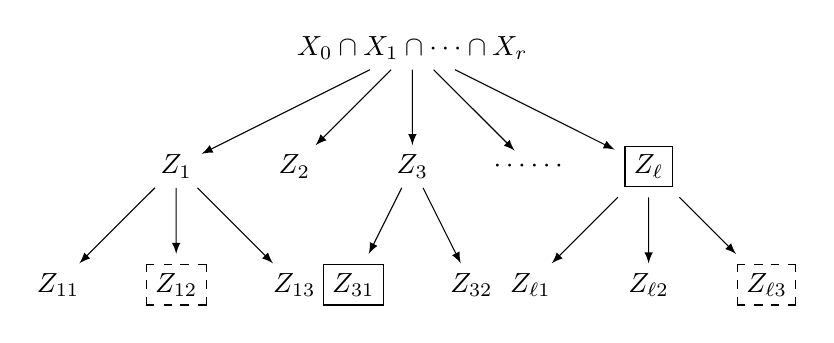
\begin{tikzpicture}[edge from parent/.style={draw,-latex}]
% [edge from parent/.style={draw, ->, thick}, level/.style={sibling distance = 30mm/#1, yshift=5cm}]
% \tikzstyle{level 2}=[sibling distance=15mm]
% \tikzstyle{level 3}=[sibling distance=5mm]
\node {$X_0\cap X_1\cap\cdots\cap X_r$} % root
child { node {$Z_1$}
child { node {$Z_{11}$} }
child { node {\dbox{$Z_{12}$}} }
child { node {$Z_{13}$} }
}
child { node {$Z_2$}
}
child { node {$Z_3$}
child { node {$\boxed{Z_{31}}$} }
child { node {$Z_{32}$} }
}
child { node {$\cdots\cdots$}
}
child { node {$\boxed{Z_{\ell}}$}
child { node {$Z_{\ell1}$} }
child { node {$Z_{\ell2}$} }
child { node {\dbox{$Z_{\ell3}$}} }
};
\end{tikzpicture}
\caption{以$X_0\cap X_1\cap\cdots\cap X_r$的不可约分支为相交树根构成的森林}
\end{figure}
假设虚线框中的顶点$Z_{12}$对应的$\mathbb{P}_k^n$的闭子概型同时是$Z_1, Z_{\ell}\in \mathcal{C}(X_1\intersect X_r)$的子概形,而且这个子概形作为$Z_{\ell}$的子节点,是另一个虚线框中的$Z_{\ell3}$,而出现在相交树中。于是,相关的顶点$Z_1, Z_{\ell}$便是集合$\mathcal Z_*$,确切的说是集合$\mathcal Z_1$,中的元素。

再假设实线框中的顶点$Z_{31}$所对应的$\mathbb{P}_k^n$的闭子概型同时是$Z_3, Z_{\ell}\in \mathcal{C}(X_1\intersect X_r)$的子概形,但是这个子概形并未作为$Z_{\ell}$的子节点而出现,因此它便不落在集合$\mathcal Z_*$中。
\end{example}

\begin{remark}
要注意的是,在上面的例子中,$Z_1,\cdots,Z_{\ell}$才是每棵相交树的根,深度为$0$。事实上,如果我们把相交树族$\{\mathscr T_C\}_{C\in\mathcal C(X_1\intersect X_r)}$视作一个森林$\mathcal{F}_{C(X_1\intersect X_r)}$,把$X_0\cap X_1\cap\cdots\cap X_r$当成一个顶点,与森林$\mathcal{F}_{C(X_1\intersect X_r)}$中所有根相连,从而把所有相交树连接成一棵树的话,再扩展相关顶点以及边的权重的定义,某些式子能得到简化,例如不等式\eqref{no auxillary scheme}左边不再需要求和,变成只有一项,但是抽象的相交树的定义相关的叙述会变得更繁琐和不统一。于是,本文还是尊重最初提出相交树的~\inlinecite{Liu-multiplicity}中的定义。
\end{remark}

\begin{remark}
我们特别地将集合$\mathcal Z_*$从集合$\mathcal C_*$中拿出来考虑,是因为被丢弃的那些顶点对应的闭子概型中点的重数已经在别处得到了计算与控制,例如上例中的$Z_{31}$与$Z_{\ell}$,因此我们不重复计算。
\end{remark}

\begin{definition}
令$t$为一个非负整数。我们将集合$\mathcal C_t$,$\mathcal Z_t$,$\mathcal C_*$以及$\mathcal Z_*$中的元素(相交树的顶点)所对应的标签构成的集合分别记为$\mathcal C'_t$,$\mathcal Z'_t$,$\mathcal C'_*$以及$\mathcal Z'_*$。
\end{definition}

下面我们要给出关于我们以上定义的集合的一个重要的性质。这个性质是定理\ref{mult in the intersection tree}的推论,将会直接用于我们所考虑的重数计数问题的证明。

\begin{proposition}[\inlinecite{Liu-multiplicity}, Proposition 4.6] \label{grassmanne}
我们保持定理\ref{mult in the intersection tree}中的记号与条件不变,并假设由相交树顶点标签组成的集合$\mathcal C'_*$的每个元素(对应的基概型的整闭子概型)维数都相同,那么对每个$0\leqslant t \leqslant s$有不等式
\begin{equation} \label{relation of multiplicity and degree}
\sum_{Z\in \mathcal Z_t} \left(\prod_{i=1}^r\mu_Z(X_i)\right)\deg(Z) \leqslant \prod_{i=1}^r\deg(X_i)\prod_{j=0}^{t-1}\max_{\widetilde{M}\in \mathcal C'_j}\{\deg(\widetilde{M})\}.
\end{equation}
特别地,在上式中,如果$t=0$,我们约定$\prod\limits_{j=0}^{t-1} \max\limits_{\widetilde{M}\in \mathcal C'_j} \{\deg(\widetilde{M})\} = 1$。
\end{proposition}

\begin{proof}
由定理\ref{mult in the intersection tree},对集合$\mathcal{Z}_*$中所有的顶点$Z$有
\begin{equation}
\sum_{C\in\mathcal C(X_1\intersect X_r)} W_{\mathscr T_C}(Z)i(C;X_1\intersect X_r;\mathbb P^n_k) \geqslant \prod_{i=1}^r\mu_Z(X_i),
\end{equation}
又注意到$\mathcal{Z}_t$是$\mathcal{C}_t$子集,因此
\begin{multline}
\sum\limits_{Z\in \mathcal{Z}_t} \left( \sum_{C\in\mathcal C(X_1\intersect X_r)} W_{\mathscr T_C}(Z)i(C;X_1\intersect X_r;\mathbb P^n_k) \right)\deg(Z) \\
\leqslant \sum\limits_{Z\in \mathcal{C}_t} \left( \sum_{C\in\mathcal C(X_1\intersect X_r)} W_{\mathscr T_C}(Z)i(C;X_1\intersect X_r;\mathbb P^n_k) \right)\deg(Z)
\end{multline}
恒成立。于是想要证明不等式\eqref{relation of multiplicity and degree},我们只要证明下式即可:
\begin{align}
I_t := & \sum\limits_{Z\in \mathcal{C}_t} \left( \sum_{C\in\mathcal C(X_1\intersect X_r)} W_{\mathscr T_C}(Z)i(C;X_1\intersect X_r;\mathbb P^n_k) \right)\deg(Z) \\
& \leqslant \prod_{i=1}^r\deg(X_i)\prod_{j=0}^{t-1} \max_{\widetilde{M}\in \mathcal C'_j} \{\deg(\widetilde{M})\} =: J_t.
\end{align}

我们对$t$进行归纳证明。

当$t=0$时,$\mathcal{C}_0 = \mathcal C(X_1\intersect X_r)$,因此
\begin{equation}
W_{\mathscr T_C}(Z) = \begin{cases}
1 & \text{ 如果$Z = C$;} \\
0 & \text{ 如果$Z \neq C$.}
\end{cases}
\end{equation}
由B\'ezout 定理(定理\ref{bezout})有
\begin{equation}
I_0 = \sum_{C\in \mathcal C(X_1\intersect X_r)} i(M;X_1\intersect X_r;\mathbb P^n_k) \deg(C) = \deg(X_1)\cdots\deg(X_r) = J_0.
\end{equation}

设$t\geqslant 1$,且命题在$t-1$时成立。那么对$t$有归纳假设有
\begin{align}
J_t & = \max_{\widetilde{M} \in \mathcal C'_{t-1}} \{\deg(\widetilde{M})\} \cdot J_{t-1} \geqslant \max_{\widetilde{M}\in \mathcal C'_{t-1}} \{\deg(\widetilde{M})\} \cdot I_{t-1} \\
& = \max_{\widetilde{M}\in \mathcal C'_{t-1}} \{\deg(\widetilde{M})\} \cdot \left( \sum\limits_{Z\in \mathcal{C}_{t-1}} \left( \sum_{C\in\mathcal C(X_1\intersect X_r)} W_{\mathscr T_C}(Z)i(C;X_1\intersect X_r;\mathbb P^n_k) \right)\deg(Z) \right) \\
& \geqslant \sum\limits_{Z\in \mathcal{C}_{t-1}} \left( \sum_{C\in\mathcal C(X_1\intersect X_r)} W_{\mathscr T_C}(Z)i(C;X_1\intersect X_r;\mathbb P^n_k) \right) \deg(Z) \deg(\widetilde{Z}) \\
& = \sum\limits_{Z\in \mathcal{C}_{t-1}} \left( \sum_{C\in\mathcal C(X_1\intersect X_r)} W_{\mathscr T_C}(Z)i(C;X_1\intersect X_r;\mathbb P^n_k) \right) \cdot \sum\limits_{Z'\in \mathcal{C}(Z\cdot \widetilde{Z})} i(Z'; Z\cdot \widetilde{Z}; \mathbb P^n_k) \deg(Z') \\
& = \sum\limits_{Z'\in \mathcal{C}_{t}} \left( \sum_{C\in\mathcal C(X_1\intersect X_r)} W_{\mathscr T_C}(Z)i(C;X_1\intersect X_r;\mathbb P^n_k) \right) \deg(Z') \\
& = I_t.
\end{align}
在上式中,第三行我们用$\widetilde{Z}$表示顶点$Z$对应的标签;第四行我们再一次用到了B\'ezout 定理(定理\ref{bezout});第五行则用到了相交重数的结合性(命题\ref{associativity of intersection})。于是命题得证。
\end{proof}

\chapter{超曲面上的重数估计}
\label{chapter:main result}
为了研究射影超曲面上的重数计数问题,我们先介绍一些关于超曲面上点的重数的一些事实。

\section{超曲面截影上的重数}
设$k$为任意的一个域,$f\in k[T_0,\cdots,T_n]$为一个次数等于$\delta$的非零齐次多项式。考虑概型
\begin{equation}
X = V(f) = \proj\left(k[T_0,\cdots,T_n]/(f)\right).
\end{equation}
事实上,概型$V(f)$是$n$维射影空间$\mathbb P^n_k$的维数纯为$n-1$的闭子概型,从而是射影空间$\mathbb{P}^n_k$内的一个超曲面,被称为为由齐次多项式$f$定义的射影超曲面。可以证明,射影超曲面$X = V(f)$的次数等于定义它的齐次多项式$f$的次数$\delta$(详见参考文献~\inlinecite{GTM52}的第一章的 Proposition 7.6)。

令$\alpha\in[0,\delta]\cap \mathbb N$为一个非负整数。我们记$\mathcal{T}^{\alpha}(f)$为形如
\begin{equation}
\partial^{|I|}_{I} f := \dfrac{\partial^{|I|}f}{\partial T^I} = \dfrac{\partial^{i_0+\cdots+i_n}f}{\partial T_0^{i_0}\cdots\partial T_n^{i_n}}
\end{equation}
的齐次多项式$f$的阶数为$\alpha$的偏导数张成的$k$-线性空间,其中$I = (i_0,\cdots,i_n)\in\mathbb{N}^{n+1}$且满足$|I| = i_0+\cdots+i_n = \alpha$。线性空间$\mathcal{T}^{\alpha}(f)$中的元素都是次数等于$\delta-\alpha$的齐次多项式。

下面,我们要引入一个决定超曲面上点的重数的显式的准则。

\begin{proposition}[\inlinecite{Liu-multiplicity}, Corollaire 5.4] \label{taylor expansion}
设域$k$的特征为$0$,$X\hookrightarrow\mathbb P^n_k$为由次数等于$\delta$的齐次多项式$f$定义的超曲面,$\xi\in X$为超曲面上的一个点,$\alpha$为区间$[0,\mu_{\xi}(X)-1]$内的非负正整数。那么任取线性空间$\mathcal{T}^{\alpha}(f)$中任意一个非零元素$g$(一个次数等于$\delta-\alpha$的齐次多项式),点$\xi$总是包含在由$g$定义的超曲面$X_{\alpha,g}$上。而当$\alpha = \mu_{\xi}(X)$时,情况正好相反,总存在一个非零元素$g'\in\mathcal{T}^{\mu_{\xi}(X)}(f)$,使得点$\xi$不落在由$g'$定义的超曲面上。
\end{proposition}

\begin{remark}
特别地,如果$\mu_{\xi}(X) > 1$,也就是说点$\xi$是一个奇异点,那么对$\mathcal{T}^1(f)$的每个元素$g$来说,点$\xi$总是落在由$g$定义的超曲面上。
\end{remark}

\begin{remark}
上述命题一个直接的结果就是,对于命题中出现的超曲面$X_{\alpha,g}$,总有
\begin{equation}
\mu_{\xi}(X_{\alpha,g}X') \geqslant \mu_{\xi}(X) - \alpha, \quad \forall \alpha \in [0,\mu_\xi(X)-1].
\end{equation}
\end{remark}

\section{相交树的构造}
\label{construction of intersection trees}
由于有命题\ref{taylor expansion},我们可以构造一族相交树,或者说一个森林,用来解决我们所考虑的重数计数问题。首先,我们需要把这族相交树的根都确定下来。为了达到这个目的,我们需要以下的命题

\begin{proposition}[\inlinecite{Liu-multiplicity}, Lemme 5.8] \label{construction of roots}
设$K$为一个数域,$f\in K[T_0,\cdots,T_n]$为一个次数等于$\delta$的齐次多项式。记$V(f)$为由齐次多项式$f$定义的超曲面。如果超曲面$V(f)$的奇点集维数等于$s$,那么存在$f$的一组方向导数$g_1,\cdots, g_{n-s-1}\in\mathcal{T}^1(f)$,使得
\begin{equation}
\dim(V(f)\cap V(g_1)\cap\cdots\cap V(g_{n-s-1}))=s.
\end{equation}
换而言之,$V(f)\cap V(g_1)\cap\cdots\cap V(g_{n-s-1})$是一个完全交。
\end{proposition}

设$K,f$如以上命题中所设,我们将在以后的论述中由齐次多项式$f$定义的超曲面$V(f)$记作$X$,即
\begin{equation}
X = \proj\left(K[T_0,\cdots,T_n]/(f)\right).
\end{equation}
我们将把$X$的正则点集记作$X^{\mathrm{reg}}$,把$X$的奇点集记作$X^{\mathrm{sing}}$。此外,为了符号统一便于书写,我们还把命题\ref{construction of roots}中出现的超曲面$V(g_i)$写作$X_i$,其中$i=1,\cdots,n-s-1$。由Jacobian判别准则(详见参考文献~\inlinecite{LiuQing}的 Theorem 4.2.19),有
\begin{equation}
X^{\mathrm{sing}} \subseteq X\cap X_1\cap\cdots\cap X_{n-s-1}.
\end{equation}

我们接下来就以集合$\mathcal C(X\cdot X_{1}\intersect X_{n-s-1})$中的所有元素,也就是射影空间$\mathbb{P}_K^n$中的相交积$X\cdot X_{1}\intersect X_{n-s-1}$的所有不可约分支,为根节点,来构造森林$\mathscr{F}_{\mathcal C(X\cdot X_{1}\intersect X_{n-s-1})} = \{\mathscr T_C\}_{C\in\mathcal C(X\cdot X_{1}\intersect X_{n-s-1})}$。其中,森林中每棵(相交)树$\mathscr T_C$的下标表示它以$C\in\mathcal C(X\cdot X_{1}\intersect X_{n-s-1})$为根节点。

我们归纳地来构造相交树里深度大于等于$1$的顶点。注意到所有深度等于$0$的点,即根节点,我们都已经取好了。假设$M$是我们已经在某一个相交树$\mathscr T_C$上构造好了的一个顶点。

对于$X$的一个整的子概形$M$,我们用$M^{(a)}$来表示$M$中那些在$X$中重数等于$M$在$X$中重数的点的集合,用$M^{(b)}$来表示$M$中那些在$X$中重数大于等于等于$\mu_M(X)+1$的点的集合。用数学符号来表示,就是
\begin{gather}
M^{(a)} = \{ \xi\in M \ |\ \mu_{\xi}(X) = \mu_{M}(X) \} ,\\
M^{(b)} = \{ \xi\in M \ |\ \mu_{\xi}(X) \geqslant \mu_{M}(X)+1 \}.
\end{gather}
此外,设$L/K$为数域的扩张,我们分别记$M^{(a)}(L)$,$M^{(b)}(L)$为$M^{(a)}$,$M^{(b)}$的$L$-有理点的集合。那么有
\begin{equation}
M(L) = M^{(a)}(L)\bigsqcup M^{(b)}(L).
\end{equation}

由命题\ref{taylor expansion},容易推出$M^{(a)}$在$M$中是稠密的,因为$M^\mathrm{reg}$是在$M$中稠密的,并且$M^\mathrm{reg}$中所有点在$X$中的重数都是$\mu_M(X)$。而$M^{(b)}$的维数则要小于等于$\dim (M)-1$。

回到我们的构造。对于顶点$M$,我们把他视作$X$的整闭子概型。考虑集合$M(\overline K)$。如果它的子集$M^{(b)}(\overline K)=\emptyset$,那么我们令$M$为叶节点,它的标签取为空集。也就是说$M$没有子节点,$M$所在的相交树这一分支构造完毕。如果$M^{(b)}(\overline K)\neq\emptyset$,那么我们任取其中的一点$\xi \in M^{(b)}(\overline K)$。由集合$M^{(b)}$的定义,我们有$\mu_M(X) < \mu_{\xi}(X) \leqslant \delta$。根据命题\ref{taylor expansion},对集合$M^{(a)}(\overline K)$中取定的一点$\xi'\in M^{(a)}(\overline K)$,我们可以在齐次多项式阶数为$\delta-\mu_M(X)$的偏导数张成的$K$-线性空间中找到某个元素$h \in \mathcal{T}^{\delta-\mu_M(X)}(f)$,使得由齐次多项式$h$定义的超曲面$V(h)$不包含点$\xi'$。那么同时,$V(h)$不包含$M$的广点。通过比较$M$与$V(h)$的维数可以知道,$M$与$V(h)$是正常相交的。线性空间$\mathcal{T}^{\delta-\mu_M(X)}(f)$中的非零元都是$\mu_M(X)$次齐次多项式,因此$\deg(h) = \mu_M(X) \leqslant \delta-1$。我们将超曲面$V(h)$取作顶点$M$的标签,记为$\widetilde{M}$。我们把顶点$M$的子节点取作相交积$M\cdot\widetilde{M}$的不可约分支。顶点$M$与其子节点相连的边的权重被定义作相应的相交重数。

值得注意的是,在构造相交树的过程中,每个顶点的标签如果不是空集,那么就是一个超曲面,维数等于$n-1$,因此集合$\mathcal{C}_t$中所有元素,即所有深度等于$t$的顶点,都是$s-t$维的,其中$1\leqslant t\leqslant s$为一个正整数。于是,以上的构造会在有限步内终结。于是,依照上文所叙述的程序,我们就可以把这族相交树$\{\mathscr T_C\}_{C\in\mathcal C(X\cdot X_{1}\intersect X_{n-s-1})}$都构造出来了。需要特别指出来的是,以上对于森林$\mathscr{F}_{\mathcal C(X\cdot X_{1}\intersect X_{n-s-1})} = \{\mathscr T_C\}_{C\in\mathcal C(X\cdot X_{1}\intersect X_{n-s-1})}$的构造并不是唯一的,因为顶点标签的选取并不唯一。

\begin{remark} \label{philosophy of intersection forest}
如此构造相交树的思路可以简述如下:

为了方便,我们来考虑稍微简单一些的$K = \mathbb{Q}$时的有理点重数的计数。首先,在最简单的情况,即所有的$M \in \mathcal{C}(X\cdot X_1\intersect X_{n-s-1})$都满足$M^{(b)} = \emptyset$,那么直接有(下式中为了方便,记$X = X_0$)
\begin{align}
& \sum\limits_{\xi \in S(X;B)} \mu_{\xi}(X)(\mu_{\xi}(X)-1)^{n-s-1} \leqslant \sum\limits_M N(M;B) \prod\limits_i \mu_{M}(X_i) \\
& \ll_{n} B^{s+1} \sum\limits_M \deg(M) \cdot i(M; X_0\intersect X_{n-s-1}; \mathbb{P}^n_{\mathbb{Q}}) \\
& \ll_{n} B^{s+1} \prod\limits_i \deg(X_i) \ll_{n} \delta(\delta-1)^{n-s-1} B^{s+1} \\
& \ll_{n,K} \delta^{n-s} \max\{B, \delta-1\}^{s+1}.
\end{align}
这直接是我们想要的(有理点重数计数的)结论。

如果情况不是那么好,存在某些相交积的不可约分支$M \in \mathcal{C}(X\cdot X_1\intersect X_{n-s-1})$使得$M^{(b)}(K) \neq \emptyset$,即$M$里面有一些点,它们的重数不能被$M$的广点的重数所控制,那么上面的不等式便不成立了。上面不等式第一行的左边求和号下的$\xi$加上额外的限制条件:$\mu_{\xi}(X) = \mu_M(X)$,对$\xi \in M$,才能使上面的不等式成立。这样一来,我们只得到一个部分的估计,还剩下那些没有被估计到的点,则需要想别的办法对其重数进行控制。而这个办法,就是我们在前文构造相交树的时候采用的方法:找一个与$M$正常相交的超曲面,而且他们的交正好把这些重数不能被$M$的广点的重数所控制的点包住。然后对相交积的每个不可约分支,再次尝试用广点的重数对其他点的重数进行控制。如此重复进行下去,直到过程终止。而我们在相交树构造的过程中已经提到了,这个过程一定会在有限步内终止。
\end{remark}

\begin{remark} \label{simple facts on forest}
关于上文构造的森林$\mathscr{F}_{\mathcal C(X\cdot X_{1}\intersect X_{n-s-1})} = \{\mathscr T_C\}_{C\in\mathcal C(X\cdot X_{1}\intersect X_{n-s-1})}$,有两个需要注意到的,以后会反复使用的性质,在这里强调并列举如下:
\begin{itemize}
\item 森林中顶点的每个非空的标签对应的闭子概型(实际上也是$\mathbb{P}_K^n$中的超曲面)的次数都小于等于$\delta-1$;
\item 每棵相交树中深度等于$t$的顶点(也就是说集合$\mathcal{C}_t$中的元素)对应的闭子概型的维数都等于$s-t$。
\end{itemize}
\end{remark}

下面我们还要给一个关于集合$\mathcal Z_*$性质的关键性的引理(集合$\mathcal Z_*$的定义见前文的定义\ref{def of Z_s})。集合$\mathcal Z_*$的这个性质在接下来将要证明的我们的主定理\ref{main theorem},进行相关的估计的时候,有基础性的作用。

\begin{lemma}[\inlinecite{Liu-multiplicity}, Lemme 5.9] \label{control of singular locus}
任取概型$X$的奇异点$\xi\in X^{\mathrm{sing}}(\overline{K})$,总是至少存在集合$\mathcal Z_*$中的一个顶点$Z$,使得$\xi\in Z^{(a)}(\overline K)$。
\end{lemma}
这是一个比较关键的引理,我们下面来证明它。
\begin{proof}
我们有三个观察:
\begin{itemize}
\item 首先,正如我们在上文已经说过,由Jacobian判别准则,有
\begin{equation}
X^\mathrm{sing}\subseteq X\cap X_1\cap\cdots\cap X_{n-s-1},
\end{equation}
因此,任取射影超曲面$X$的奇异点$\xi\in X^{\sing}(\overline{K})$,总存在$Z\in\mathcal C(X\cdot X_{1}\intersect X_{n-s-1})$,使得$\xi \in Z(\overline{K})$。
\item 其次,注意到集合$\mathcal{C}_t$中顶点所对应的闭子概型的维数都等于$s-t$(见注释\ref{simple facts on forest}),而且$s\leqslant n-2$,如果集合$\mathcal{C}_{n-2}$不等于空集,里面元素(相交树的顶点)所对应的闭子概型都是$0$维的,由有限个孤立点组成。这些闭点作为$X$的既约子概形,必然是正则的。也就是说在这种情况下,任取$Z \in \mathcal{C}_{n-2}$,有$Z^{(b)} = \emptyset$。
\item 假设$t$满足$\mathcal{C}_t = \emptyset$,但$\mathcal{C}_{t-1} \neq \emptyset$,那么由定义必然有
\begin{equation}
\forall Z \in \mathcal{C}_{t-1}, ~~ Z^{(b)} = \emptyset.
\end{equation}
\end{itemize}
于是,由以上三个观察我们能得出的结论是:对任意的奇异点$\xi\in X^{\sing}(\overline{K})$,总存在某个$w$,以及$Z\in \mathcal{C}_w$使得$\xi\in Z^{(a)}(\overline{K})$。

对于一个取定的奇异点$\xi$,令$w$为满足存在$Z\in \mathcal{C}_w$使得$\xi\in Z^{(a)}(\overline{K})$的最小的整数。如果$Z$可以落在集合$\mathcal{Z}_w \subseteq \mathcal{C}_w$中,那么我们就证明完毕了。

如若不然,那么对任意满足$\xi\in Z^{(a)}(\overline{K})$的$Z\in \mathcal{C}_w$,都有$Z\not\in \mathcal{Z}_w$。那么存在满足下面两个条件的极大的$w'$:
\begin{itemize}
\item $w' < w$;
\item 存在$Z' \in \mathcal{C}_{w'}$,使得$Z\subsetneqq Z'$,而且作为森林$\mathscr{F}_{\mathcal C(X\cdot X_{1}\intersect X_{n-s-1})}$中的顶点,$Z$不是$Z'$的子孙。
\end{itemize}
如果$\xi\in Z'^{(a)}(\overline{K})$,那么这会与$w$的极小性相矛盾。如果$\xi\in Z'^{(b)}(\overline{K})$,那么会有
\begin{equation}
\mu_{\eta_Z}(X) = \mu_Z(X) = \mu_{\xi}(X) > \mu_{Z'}(X) = \mu_{\eta_{Z'}}(X),
\end{equation}
其中$\eta_Z$与$\eta_{Z'}$分别为$Z$与$Z'$的广点。根据上文有关相交树的构造,特别是关于其构造思路的注释\ref{philosophy of intersection forest},我们知道$Z$一定会是$Z'$的子孙,这与$w'$的取法矛盾。证明完毕。
\end{proof}

\begin{remark}
引理\ref{control of singular locus}在刘春晖文章~\inlinecite{Liu-multiplicity}中是在有限域上证明的。事实上,这个结论在数域上仍然是成立的,因为文章~\inlinecite{Liu-multiplicity}中对这个引理的证明用到基域$k$的性质的地方,仅仅在于要求它是一个完全域。
\end{remark}

\section{重数的计数}
\label{counting multiplicity}
我们沿用本章的常用的记号。以下便是我们要证明的主定理的叙述

\begin{theorem} \label{main theorem}
令$K$为一个数域,$n \geqslant 2$,$\delta \geqslant 1$以及$s \geqslant 0$为整数。那么以下的不等式
\begin{equation} \label{estimate in main theorem}
\sum_{\xi\in S(X;D,B)} \mu_{\xi}(X)(\mu_{\xi}(X)-1)^{n-s-1} \leqslant \sum_{t=0}^s\max_{Z\in\mathcal Z_t}\left\{\frac{N(Z;D,B)}{\deg(Z)}\right\}\delta(\delta-1)^{n-s+t-1}.
\end{equation}
% \begin{eqnarray*}& &\sum_{\xi\in S(X;D,B)} \mu_{\xi}(X)(\mu_{\xi}(X)-1)^{n-s-1}\\
% &\leqslant&\sum_{t=0}^s\max_{Z\in\mathcal Z_t}\left\{\frac{N(Z;D,B)}{\deg(Z)}\right\}\delta(\delta-1)^{n-s+t-1}.\end{eqnarray*}
对于$P^n_K$中所有次数等于$\delta$,且奇点集维数等于$s$的既约的射影超曲面$X$都是成立的。上式中,符号$S(X;D,B)$与$N(X;D,B)$的定义分别在在式\eqref{S(X;D,B)}与式\eqref{N(X;D,B)}中给出,集合$\mathcal{Z}_t$的定义在定义\ref{def of Z_s}中给出。特别地,如果某个$\mathcal{Z}_t = \emptyset$,$0 \leqslant t \leqslant s$,那么我们约定$\max\limits_{Z\in\mathcal Z_t} \left\{ \frac{N(Z;D,B)}{\deg(Z)} \right\} = 0$。
\end{theorem}

\begin{proof}
对于$P^n_K$中任意的一个次数等于$\delta$,奇点集维数等于$s$的既约的射影超曲面$X$,我们假设已经由\S \ref{construction of intersection trees}中所描述的程序构造好了森林$\mathscr{F}_{\mathcal C(X\cdot X_{1}\intersect X_{n-s-1})} = \{\mathscr T_C\}_{C\in\mathcal C(X\cdot X_{1}\intersect X_{n-s-1})}$,使得森林中每棵相交树的根都来自集合$\mathcal C(X\cdot X_{1}\intersect X_{n-s-1})$。

首先,对于我们想要证明的不等式的左边,由于超曲面$X$中正则点的重数都等于$1$,于是我们有
\begin{equation} \label{first step}
\sum\limits_{\xi\in S(X;D,B)} \mu_\xi(X)(\mu_\xi(X)-1)^{n-s-1} = \sum\limits_{\xi\in S(X^\mathrm{sing};D,B)} \mu_\xi(X)(\mu_\xi(X)-1)^{n-s-1}.
\end{equation}

由引理\ref{control of singular locus},任取超曲面$X$上的一个奇异点$\xi\in X^{\mathrm{sing}}(\overline K)$,我们总能找到一个顶点,或者说一个闭子概型,$Z\in\mathcal{Z}_*$,使得$\xi\in Z^{(a)}(\overline K)$,因此我们又有
% \begin{equation} \label{final 1}
% \sum\limits_{\xi\in S(X^\mathrm{sing};D,B)}\mu_\xi(X)(\mu_\xi(X)-1)^{n-s-1} \leqslant \sum_{t=0}^{s} \sum_{Z\in\mathcal Z_t} \sum_{\xi\in S(Z^{(a)};D,B)} \mu_\xi(X)(\mu_\xi(X)-1)^{n-s-1}.
% \end{equation}
\begin{multline} \label{final 1}
\sum\limits_{\xi\in S(X^\mathrm{sing};D,B)} \mu_\xi(X)(\mu_\xi(X)-1)^{n-s-1}\\
\leqslant \sum_{t=0}^{s} \sum_{Z\in\mathcal Z_t} \sum_{\xi\in S(Z^{(a)};D,B)} \mu_\xi(X)(\mu_\xi(X)-1)^{n-s-1}.
\end{multline}

又由命题\ref{taylor expansion},对于每个$Z\in\mathcal Z_*$,我们有不等式
\begin{equation}
\mu_Z(X)-1\leqslant\mu_Z(X_i),
\end{equation}
对$i=1,\cdots,n-s-1$都成立。于是我们有不等式
\begin{equation} \label{final_1'}
\mu_Z(X)(\mu_Z(X)-1)^{n-s-1} \leqslant \mu_Z(X)\mu_Z(X_{1})\cdots\mu_Z(X_{n-s-1}).
\end{equation}

根据命题\ref{grassmanne}以及上面的不等式\eqref{final_1'},对于每个$t=0,\cdots,s$,我们有
\begin{align} \label{final 2}
& \sum_{Z\in\mathcal Z_t} \mu_Z(X)(\mu_Z(X)-1)^{n-s-1}\deg(Z) \nonumber \\
& \leqslant \sum_{Z\in\mathcal Z_t} \mu_Z(X)\mu_Z(X_{1})\cdots\mu_Z( X_{n-s-1})\deg(Z) \\
& \leqslant \deg(X)\prod_{i=1}^{n-s-1}\deg(X_i)\prod_{j=0}^{t-1}\max_{\widetilde{Z}\in \mathcal C'_t}\{\deg(\widetilde{Z})\} \\
& \leqslant \delta(\delta-1)^{n-s+t-1}.
\end{align}
这是因为集合$\mathcal C'_*$中所有的元素(相交树上顶点的标签,也是闭子概型)的次数都是小于等于$\delta-1$的。

把不等式\eqref{final 1}和不等式\eqref{final 2}结合起来看,便有
\begin{align} \label{final step}
& \sum_{t=0}^{s} \sum_{Z\in\mathcal{Z}_t} \sum_{\xi\in S(Z^{(a)};D,B)} \mu_\xi(X)(\mu_\xi(X)-1)^{n-s-1} \nonumber \\
= & \sum_{t=0}^{s} \sum_{Z\in\mathcal{Z}_t} \mu_Z(X)(\mu_Z(X)-1)^{n-s-1}N(Z^{(a)};D,B) \\
\leqslant & \sum_{t=0}^{s} \sum_{Z\in\mathcal{Z}_t} \mu_Z(X)(\mu_Z(X)-1)^{n-s-1}N(Z;D,B) \\
\leqslant & \sum_{t=0}^{s} \max_{Z\in\mathcal{Z}_t} \left\{\frac{N(Z;D,B)}{\deg(Z)}\right\} \left(\sum_{Z\in\mathcal{Z}_t} \mu_Z(X)(\mu_Z(X)-1)^{n-s-1}\deg(Z)\right) \\
\leqslant & \sum_{t=0}^s \max_{Z\in\mathcal{Z}_t} \left\{\frac{N(Z;D,B)}{\deg(Z)}\right\} \delta(\delta-1)^{n-s+t-1}.
\end{align}
把不等式\eqref{first step},\eqref{final 1}以及\eqref{final step}综合起来,就得到了我们想要证明的不等式。定理证毕。
\end{proof}

\section{有理点重数的计数}
在这一小节中,我们考虑定理\ref{main theorem}的一种相对简单一些的特殊情况,即有理点重数的计数问题。结合之前我们得到的关于一般化的 Schanuel 估计的一个一致性的结果,我们将要得到一个比原定理稍微精细一些的结果。自然,这个结果也是一个一致性的估计。

\begin{corollary} \label{main corollary}
设$n \geqslant 2$,$\delta \geqslant 1$以及$s \geqslant 0$为整数。那么以下的估计
\begin{equation} \label{estimate in main corollary}
\sum_{\xi\in S(X;B)} \mu_\xi(X)(\mu_\xi(X)-1)^{n-s-1} \ll_{n} \delta^{n-s}\max\{B,\delta-1\}^{s+1}.
\end{equation}
对于$\mathbb{P}^n_{\mathbb{Q}}$中所有次数等于$\delta$,且奇点集维数等于$s$的既约的射影超曲面$X$都是成立的。
\end{corollary}

\begin{proof}
% 由\S\ref{construction of intersection trees}中相交树的构造,集合$\mathcal{Z}_t, t=0,\cdots,s$,的每个元素$Z$都是一个局部完全交。再结合注释\ref{degree 1 estimate}中的论述,我们有如下的估计
对于$\mathbb{P}^n_{\mathbb{Q}}$中任何一个次数等于$\delta$,且奇点集维数等于$s$的既约的射影超曲面$X$,假设已经由\S \ref{construction of intersection trees}中所描述的程序构造好了森林$\mathscr{F}_{\mathcal C(X\cdot X_{1}\intersect X_{n-s-1})} = \{\mathscr T_C\}_{C\in\mathcal C(X\cdot X_{1}\intersect X_{n-s-1})}$,使得森林中每棵相交树的根都来自集合$\mathcal C(X\cdot X_{1}\intersect X_{n-s-1})$。考虑我们在定义\ref{def of Z_s}中特别取出来的森林中的顶点的子集$\mathcal{Z}_t$,对于每一个$Z \in \mathcal{Z}_t$,$t = 0,\ldots,s$,由定理\ref{refined Schanuel estimate for rational points}我们有估计$N(Z;B) = \#S(Z;B) \ll_{n} \deg(Z) B^{\dim(Z)+1}$,亦即
\begin{equation}
\frac{N(Z;B)}{\deg(Z)} \ll_{n} B^{\dim(Z)+1}, \quad B \geqslant 1.
\end{equation}
把这个估计代入上一小节证明的主定理\ref{main theorem}中,结合集合$\mathcal{C}_t$中(因此,集合$\mathcal{Z}_t$中)的每个顶点$Z$的维数$\dim(Z) = s - t$以及$s \leqslant n-2$的事实,我们有
\begin{eqnarray}
& & \sum_{\xi\in S(X;B)} \mu_\xi(X)(\mu_\xi(X)-1)^{n-s-1} \nonumber \\
& \leqslant & \sum_{t=0}^s \max_{Z\in\mathcal Z_t}\left\{\frac{N(Z;B)}{\deg(Z)}\right\}\delta(\delta-1)^{n-s+t-1} \\
& \ll_{n} & \sum_{t=0}^s B^{s-t+1}\delta(\delta-1)^{n-s+t-1} \\
& \leqslant & \begin{cases}
\delta(\delta-1)^n \sum\limits_{t=1}^{s+1} \left(\dfrac{B}{\delta-1}\right)^t & \text{若$B > \delta - 1$} \\
\delta(\delta-1)^{n-s-1}B^{s+1} \sum\limits_{t=0}^{s} \left(\dfrac{\delta-1}{B}\right)^t & \text{若$B < \delta - 1$} \\
\delta(\delta-1)^n(s+1) & \text{若$B = \delta - 1$}
\end{cases} \\
& \leqslant & \delta(\delta-1)^{n-s-1} \max\{B,\delta-1\}^{s+1} (s+1) \\
& \leqslant & (n-1) \delta^{n-s} \max\{B,\delta-1\}^{s+1} \\
& \ll_{n} & \delta^{n-s}\max\{B,\delta-1\}^{s+1}.
\end{eqnarray}
于是我们得到了想要证明的估计式\eqref{estimate in main corollary}。
\end{proof}

下面我们做一个注记,阐述关于我们为什么要选取$f(x) = x(x-1)^{n-s-1}$作为我们的计数函数。

\begin{remark}
以下的记号的意义与定理\ref{main theorem}以及推论\ref{main corollary}中保持一致。如果不考虑常数乘子的话,只有计数函数(或者说计数多项式)的次数对我们的结果有影响。事实上,设函数$f:\mathbb N^+\rightarrow \mathbb N$为任意的增的多项式函数,次数为$t+1$且满足$f(1)=0$,那么存在一个依赖于$f$的常数$C_f$使得$f(x)\leqslant C_fx(x-1)^t$。从而有
\begin{eqnarray}
\sum_{\xi\in S(X;D,B)} f(\mu_\xi(X)) & \leqslant & C_f \sum_{\xi\in S(X;D,B)} \mu_\xi(X)(\mu_\xi(X)-1)^t \nonumber \\
& \ll_f & \sum_{\xi\in S(X;D,B)} \mu_\xi(X)(\mu_\xi(X)-1)^t.
\end{eqnarray}

不久我们就会通过一个例子(例\ref{cylinder})看到,当$t\geqslant n-s-1$的时候,上式右边$\sum\limits_{\xi\in S(X;D,B)} \mu_\xi(X)(\mu_\xi(X)-1)^t$的上界估计有类似推论\ref{main corollary}中得到的估计式\eqref{estimate in main corollary}右边那样的表达式,而且各个因子的指数都是最优的。当$t<n-s-1$时,我们目前能说的只有一个平凡的估计
\begin{equation}
\sum\limits_{\xi\in S(X;B)}\mu_\xi(X)(\mu_\xi(X)-1)^t \leqslant \sum\limits_{\xi\in S(X;B)}\mu_\xi(X)(\mu_\xi(X)-1)^{n-s-1},
\end{equation}
暂时没有别的更好的结果。

因此,如果我们在上述估计中,不关心依赖于函数$f$的常数,那么选取$f(x)=x(x-1)^{n-s-1}$作为我们的计数函数对于我们来说便是足够的,正如我们在定理\ref{main theorem}中所做的那样。

设$g:\mathbb N^+\rightarrow\mathbb N$是另一个计数函数,递增,但不再满足$g(1)=0$。那么有
\begin{align}
\sum_{\xi\in S(X;D,B)} g(\mu_\xi(X)) & = g(1)N(X^{\mathrm{reg}};D,B) + \sum_{\xi\in S(X;D,B)} \left(g(\mu_\xi(X))-g(1)\right) \nonumber \\
& \leqslant g(1)N(X;D,B) + \sum_{\xi\in S(X;D,B)} \left(g(\mu_\xi(X))-g(1)\right).
\end{align}
考虑上式中的求和项$\sum\limits_{\xi\in S(X;D,B)} \left(g(\mu_\xi(X))-g(1)\right)$,它便等价于用一个满足$f(1)=0$的计数函数来对重数进行计数的问题,这是我们之前已经讨论过的。而上式中的另一项$g(1)N(X;D,B)$,如果不考虑常数$g(1)$的话,便直接是概型上代数点、有理点计数的估计这一经典的问题。关于这一问题,我们之前也已经有过了介绍以及讨论。由$X^\mathrm{reg}$与$X$是双有理等价的这一事实,我们用定理\ref{main theorem}中所选的计数函数所做出的估计是合适的。
\end{remark}

\section{一些例子}

接下来,我们给一些例子,来具体说明我们所做出过的一些论断。

\begin{example} \label{cylinder}
令$X'\hookrightarrow\mathbb P^2_{\mathbb{Q}}$一个次数等于$\delta$的既约射影平面曲线,可以由$\delta$次齐次多项式$f(T_0,T_1,T_2)$定义。我们假设$X'$有一个重数等于$\delta$的${\mathbb{Q}}$-有理点。$\delta$次齐次多项式$f(T_0,T_1,T_2)$同时也可以视作是多项式环${\mathbb{Q}}[T_0,\cdots,T_n]$中的一个$\delta$次齐次多项式。我们把$n$维射影空间$\mathbb P^n_{\mathbb{Q}}$中由$f$定义的超曲面记作$X$。不妨设平面射影曲线$X'$的奇异点射影坐标为$[1:0:0]$,那么有
\begin{align}
X^{\mathrm{sing}}(\mathbb{Q}) = & \{[x_0:\cdots:x_n] \in \mathbb{P}^n_{\mathbb{Q}}(\mathbb{Q}) \ |\ x_0:x_1:x_2 = 1:0:0 \} \cup \nonumber\\
& \{[x_0:\cdots:x_n] \in \mathbb{P}^n_{{\mathbb{Q}}}({\mathbb{Q}}) \ |\ x_0=x_1=x_2=0\},
\end{align}
并且$X^{\mathrm{sing}}(\mathbb{Q})$中所有(有理奇异)点的重数都等于$\delta$。由渐进估计式\eqref{Schanuel over Q},我们有
\begin{equation}
N(X^{\mathrm{sing}};B) = N(\mathbb{P}^{n-2}_{\mathbb{Q}};B) = \frac{2^{n-2}}{\zeta(n-1)} B^{n-1} + o(B^{n-1}), \quad B \rightarrow +\infty,
\end{equation}
从而有下列关于重数计数的渐进估计
\begin{equation*}
\sum\limits_{\xi \in S(X;B)} \mu_\xi(X)(\mu_\xi(X)-1) = \delta(\delta-1) N(X^{\mathrm{sing}};B) = O_{n} \left( \delta^2 B^{n-1} \right).
\end{equation*}
% 那么有
% \begin{equation}
% \sum\limits_{\xi \in S(X;B)} \mu_\xi(X)(\mu_\xi(X)-1) \sim_{n} \delta^2B^{n-1}.
% \end{equation}

结合这个例子我们便可以看出,当$\dim(X^\mathrm{sing}) = n-2$且$n \geqslant 3$时,推论\ref{main corollary}中估计式右边的$\delta$的阶数是最优的。更一般地,如果$X^\mathrm{sing}$包含了一个重数等于$\delta$的线性集,那么在推论\ref{main corollary}中,当$B \geqslant \delta-1$,重数的计数$\sum\limits_{\xi\in S(X;B)} \mu_\xi(X)(\mu_\xi(X)-1)$能达到$\delta$和$B$的阶数能取到(推论\ref{main corollary}估计式右边)的最大值。
\end{example}

% 当射影超曲面$X$的奇点集$X^{\mathrm{sing}}$的所有不可约分支的次数都严格大于$1$的时候,我们可以利用本文\S\ref{HB conjecture}中提到的一些结果,来得到对$\max\limits_{Z\in\mathcal Z_t}\left\{\frac{N(Z;B)}{\deg(Z)}\right\}$的比推论\ref{main corollary}中更佳的估计,从而对
% \begin{equation}
% \sum_{\xi\in S(X;B)}\mu_\xi(X)(\mu_\xi(X)-1)^{n-s-1}
% \end{equation}
% 给出更优的估计。

设$K$为一个一般的数域,$X \hookrightarrow \mathbb{P}^n_K$为任意一个次数等于$\delta$的超曲面。想要利用定理\ref{main theorem}来解决这种更加一般的重数计数问题,关键在于给出定理估计式\eqref{estimate in main theorem}中的项
\begin{equation}
\max_{Z \in \mathcal{Z}_t} \left\{ \frac{N(Z;D,B)}{\deg(Z)} \right\}
\end{equation}
的一致的估计,其中$Z \in \mathcal{Z}_t$,$t = 1,\ldots,s$,$\mathcal{Z}_t$仍是由$X$出发构造的相交树的特定的顶点之集,具体定义可以回顾定义\ref{def of Z_s}。

在定理\ref{refined Schanuel estimate for rational points}中,我们已经仔细考察了$K = \mathbb{Q}$的情形,并且由此定理证明了推论\ref{main corollary}中的结论。如果$X$的奇点集$X^{\mathrm{sing}}$的所有不可约分支的次数都是严格大于$1$的,那么我们就可以利用我们在\S\ref{HB conjecture}中介绍的一些结果来得到关于
\begin{equation}
\sum_{\xi \in S(X;B)} \mu_\xi(X)(\mu_\xi(X)-1)^{n-s-1}
\end{equation}
比在推论\ref{main corollary}中更加精细的一些估计。其原因在于,在这种情况下,对于
\begin{equation}
\max\limits_{Z\in\mathcal{Z}_t} \left\{ \frac{N(Z;B)}{\deg(Z)} \right\},
\end{equation}
我们有比定理\ref{refined Schanuel estimate for rational points}更优的估计。

\begin{example} \label{example using HB conj}
设$\delta \geqslant 3$以及$n \geqslant 2$为正整数,令
\begin{equation} \label{hypersurface Z}
\begin{tikzcd}
Z \arrow[r, hookrightarrow] & \mathbb{P}^{n+2}_{\mathbb{Q}} = \proj\left(\mathbb{Q}[X,Y,T_0,\cdots,T_n]\right)
\end{tikzcd}
\end{equation}
是一个由$\delta$次齐次多项式
\begin{equation} \label{hypersurface Z2}
F(X,Y,T_0,\cdots,T_n) = Y^\delta + Xf(T_0,T_1,\cdots,T_n)
\end{equation}
定义的超曲面,其中$f(T_0,\cdots,T_n)$是一个$\delta-1$次齐次多项式。我们假设$f$在$P^{n}$中定义了一个光滑的超曲面,我们把它记作$Z'$。那么多项式$F(X,Y,T_0,\cdots,T_n)$是不可约的。由参考文献~\inlinecite{LiuQing}的习题2.4.1可知,超曲面$Z$是整的。由参考文献~\inlinecite{Browning_Heath06II}的 Theorem 1,当$\delta \geqslant 3$且$n \geqslant 2$时,对任意的$\epsilon>0$,估计式
\begin{equation} \label{N(Z';B)}
N(Z';B) \ll_{K,n,\delta,\epsilon} B^{n-1+\epsilon}.
\end{equation}
对所有的这样的光滑超曲面$Z'$都是成立的。

与此同时,由Jacobian判别准则(详见参考文献~\inlinecite{LiuQing}第4章的Theorem 2.19),超曲面$Z$的奇点集由下列方程组给出
\begin{equation}
\begin{cases}
\delta Y^{\delta-1} = 0 \\
f(T_0,\cdots,T_n) = 0 \\
X \frac{\partial f}{\partial T_0} = 0 \\
\phantom{hehe} \vdots \\
X \frac{\partial f}{\partial T_n} = 0
\end{cases}
\end{equation}
% $$0 = \delta Y^{\delta-1} = f(T_0,\cdots,T_n) = X\frac{\partial f}{\partial T_0} = \cdots = X\frac{\partial f}{\partial T_n}.$$
由于超曲面$Z'$在$\mathbb{Q}$上是光滑的,因此多项式$f, \frac{\partial f}{\partial T_0}, \cdots, \frac{\partial f}{\partial T_n}$没有公共零点。所以,任取超曲面$Z$上的奇异点$\xi\in Z^{\mathrm{sing}}(\overline{\mathbb{Q}})$,其射影坐标,设为$[x:y:t_0:\cdots:t_n]$,必须满足如下条件
\begin{equation}
\begin{cases}
x = y = 0 \\
[t_0:\cdots:t_n] \in Z'(\overline{\mathbb{Q}})
\end{cases}
\end{equation}
% $$X=Y=0, ~~ \text{ 且 } ~~ [T_0:\cdots:T_n] \in X'(\overline K).$$
容易看出,这些奇异点在超曲面$Z$中的重数都是$2$。由定义,超曲面$Z$的奇点集$Z^\mathrm{sing}$在$Z$中的余维数等于$2$,也就是说它的维数等于$n-1$。

我们把在定理\ref{main theorem}中考察过的问题应用到本例中来。具体来说,我们要考察和式$\sum\limits_{\xi \in S(Z;B)} \mu_{\xi}(Z)(\mu_{\xi}(Z)-1)^2$。对于本例来说,首先,对于任意的正整数$\delta \geqslant 3$和$n \geqslant 2$,以及任意的正实数$\epsilon > 0$,所用通过\eqref{hypersurface Z},\eqref{hypersurface Z2}中的方法定义的超曲面$Z,Z'$,我们都有
\begin{equation}
\sum_{\xi \in S(Z;B)} \mu_{\xi}(Z)(\mu_{\xi}(Z)-1)^2 = 2N(Z';B).
\end{equation}
假设我们依照\S\ref{construction of intersection trees}中的程序来构造(一族)相交树的话,我们会发现,我们只能得到一颗相交树,而且这个相交树里面只有根节点,即$Z$,$V \left(\frac{\partial F}{\partial X}\right)$,$V \left(\frac{\partial F}{\partial Y}\right)$的(正常)相交积,这个根节点没有任何的子孙。这是一种退化了的情况。把定理\ref{main theorem}的结果直接套用在这个例子上,我们会有
\begin{equation}
\sum_{\xi \in S(Z;B)} \mu_{\xi}(Z)(\mu_{\xi}(Z)-1)^2 \leqslant \delta(\delta-1)^2 \frac{N(Z';B)}{\delta-1} = \delta(\delta-1)N(Z';B).
\end{equation}
这正好达到了我们在定理\ref{main theorem}中给出的估计的上界。

% 而根据参考文献~\inlinecite{Browning_Heath06II}中 Theorem 1,我们
% \begin{equation}
% \sum_{\xi \in S(X;B)} \mu_{\xi}(X)(\mu_{\xi}(X)-1)^2 = 2N(X;B) \ll_{K,n,\delta,\epsilon} B^{n-1+\epsilon},
% \end{equation}
% 对任意的$\epsilon>0$成立。这个例子表明,在定理\ref{main theorem}的估计式\eqref{estimate in main theorem}中的上界是能够达到的。

而根据参考文献~\inlinecite{Browning_Heath06II}的 Theorem 1给出的非奇异超曲面上有理点的估计式\eqref{N(Z';B)},对于所用通过\eqref{hypersurface Z},\eqref{hypersurface Z2}中的方法定义的超曲面$Z, Z'$,我们都有估计
\begin{equation}
\sum_{\xi \in S(Z;B)} \mu_{\xi}(Z)(\mu_{\xi}(Z)-1)^2 = 2N(Z';B) \ll_{n,\delta,\epsilon} B^{n-1+\epsilon}.
\end{equation}
相对于我们在推论\ref{main corollary}中给出的估计,上述估计式给出了对于$B$的阶数更优的估计。然而在这个估计中,并没有对超曲面次数$\delta$在估计式中的阶进行讨论,而且就作者目前的知识而言,通过这种方法在相关的估计中还无法对$\delta$的阶进行控制。

% 并没有对超曲面次数$\delta$在估计式中的阶进行讨论,就作者目前的知识而言,本文在相关的估计中还无法对$\delta$的阶进行控制。
\end{example}

% 至于一般的代数点的重数计数问题,如果相应的次数,维数满足\S\ref{counting algebraic points in Pn}中列出来的那些条件,那么仿照证明推论\ref{main corollary}的方法,我们也能够由定理 \ref{refined Schanuel estimate for rational points}得到类似的一些估计。

\section{问题的推广}
本文所解决的问题是针对数域上射影超曲面的,我们也可以在一个一般的射影算术簇$X$上考虑上面的代数点、有理点的重数计数的问题。但是情况会复杂很多。

仿照参考文献~\inlinecite{Liu-multiplicity}中提出的猜想,本文也提出类似的猜想

\begin{conjecture}
令$X$是$n$维射影空间$\mathbb P^n_K$的一个既约的纯维数的闭子概型。令$X$的维数等于$d$,次数等于$\delta$,假设$X$的奇点集$X^{\mathrm{sing}}$的维数等于$s$。那么有
\begin{equation}
\sum_{\xi\in S(X;B)} \mu_\xi(X)(\mu_\xi(X)-1)^{d-s} \ll_{n,K} \delta^{d-s+1}B^{s+1}.
\end{equation}
\end{conjecture}



%%% 其它部分
\backmatter

% %% 本科生要这几个索引,研究生不要。选择性留下。
% % 插图索引
% \listoffigures
% % 表格索引
% \listoftables
% % 公式索引
% \listofequations


%% 参考文献
% 注意:至少需要引用一篇参考文献,否则下面两行可能引起编译错误。
% 如果不需要参考文献,请将下面两行删除或注释掉。
\bibliographystyle{thuthesis-numerical}
\bibliography{ref/refs}


%% 致谢
% 如果使用声明扫描页,将可选参数指定为扫描后的 PDF 文件名,例如:
% \begin{ack}[scan-statement.pdf]
\begin{acknowledgement}
  首先,我衷心感谢我的前任导师印林生教授(1963.12.12 - 2015.7.5)。是他把我引入了神奇的数论世界。他的言传身教将使我终生受益。我要感谢印林生教授的妻子,我的师母李平老师,在生活上一直以来的对我的无微不至的关怀。

  我衷心感谢导师张贺春教授对本人的精心指导和关怀。没有他的鼓励、帮助与鞭策,我不可能重新开始已停顿已久的研究工作,顺利完成博士学业。

  我想感谢刘春晖博士,把 Counting Multiplicities in a Hypersurface 这个课题介绍给我。他对这个问题已经在有限域的情形下做了许多卓越的工作,特别是首次提出的相交树的概念,给相关问题打下了坚实的基础,大大方便了研究工作。他的博闻强识以及对待学问严肃认真的态度,让我受益匪浅。

  我要感谢我的父母,我的妻子,我的岳母还有我的女儿。在我困顿的时候给我鼓励与支持,让我没有后顾之忧,能够斗志旺盛,全身心地投入到博士课题的研究中。

  我要感谢姚家燕教授,引领我入门代数几何,让我习得法国 Bourbaki 学派的治学精神。虽然不是他的学生,但是他总是毫无保留地给予我各种帮助。

  我还要感谢阳恩林博士,杨炯博士,曾锦骧博士,宋元龙,曹阳,孙理老师,李修美老师,张翀老师,熊玮老师,孙晟昊老师,唐舜老师,陈华一教授,徐飞教授,翁林教授,田野教授及其讨论班上的所有老师同学,还有许多我不知道名字的同行。每次和他们讨论问题,或是聆听他们的课程、报告,总能使我收获颇多。

  在法国波尔多一大(现波尔多大学)数学系进行六个月的访问学习期间,承蒙刘青教授热心指导与帮助,不胜感激。在波尔多期间,沙敏博士与童纪龙教授在研究上与生活上都给了我非常多的帮助,我非常感谢他们。我要感谢清华大学的短期访学基金在这个项目上给我的资助。我还要感谢我在那里的朋友 Andrea Siviero,每周组织球赛,丰富了我的生活,让我结识了许多有趣的人。

%   最后,我要感谢 \thuthesis,它的存在让我的论文写作轻松自在了许多,让我的论文格式规整漂亮了许多。
\end{acknowledgement}


%% 附录
\begin{appendix}
\chapter{数论的一些基础知识}
\label{apdx: number theory}
在这个附录中,我们将介绍一些本文需要用到的数论的一些知识,并对正文中简要提及的内容做一定的补充。主要的参考文献是~\inlinecite{YinLinsheng},~\inlinecite{LiJinghui}以及~\inlinecite{LangANT}。
\section{域的有限扩张的 Galois 理论}
\label{apdx: galois theory}
设$K$为域,$L/K$为有限扩域,也就是说作为$K$-线性空间,$L$是有限维的。此维数被记作$[L:K]$,被称为$L/K$的扩张次数。称$L$的一个自同构$\sigma: L \to L$为一个$K$-自同构,如果$\sigma|_K = \identity_K$,即$\sigma$限制在$K$上是恒等映射。记$L$所有的$K$-自同构组成的集合为$\aut_K(L)$。以映射的复合作为乘积运算,则$\aut_K(L)$构成一个群。一般地,$\#\aut_K(L) \leqslant [L:K]$。如果等号成立,则称$L/K$为 Galois 扩张,而把$\aut_K(L)$记为$\gal(L/K)$,称为域扩张$L/K$的 Galois 群。

一个更一般的,对无限扩张也适用的定义是
\begin{definition}
设$L/K$是域的代数扩张。若它是可分且正规的,那么称域扩张$L/K$为 Galois 扩张。
\end{definition}
这里,$L/K$是代数扩张指的是,对$L$中任一个元素$a$,都存在多项式$f_a(X) \in K[X]$使得$f_a(a)=0$。记这些多项式中次数最低的首一的多项式(从而必然不可约)为$m_a(X)$,称为$a$的极小多项式。代数扩张$L/K$是可分的指的是,对$L$中任一个元素$a$,其极小多项式$m_a(X)$无重根;代数扩张$L/K$是正规的,指的是$L$包含$a$的所有共轭元,即$m_a(X)$的所有根。

有限 Galois 扩张的 Galois 群与中间域有如下关系,被称为有限 Galois 扩张的主定理。
\begin{theorem}[\inlinecite{YinLinsheng}, 定理 B.3]
\label{galois main theorem}
设$L/K$为域的有限 Galois 扩张,并令$G = \gal(L/K)$。那么有集合间的双射
\begin{equation}
\{ \text{使$K\subseteq M \subseteq L$的域$M$} \} \overset{1:1}{\longleftrightarrow} \{ \text{$G$的子群$H$} \}
\end{equation}
其中
\begin{gather*}
H = \{ \sigma \in G \ |\ \text{对所有的$x\in M$使得$\sigma(x) = x$} \}, \\
M = \{ x\in L \ |\ \text{对所有的$\sigma\in H$使得$\sigma(x) = x$} \}.
\end{gather*}
\end{theorem}

关于域的有限扩张,有两个基本而且重要的映射:迹映射与范映射。

\begin{definition}
设$L/K$为域的有限扩张,$a\in L$,考虑$K$-线性映射
$$L \longrightarrow L: x\mapsto ax.$$
分别定义$N_{L/K}(a)$与$\tr_{L/K}(a)$为以上线性映射的行列式与迹。
\end{definition}

迹与范的基本性质可以列举如下

\begin{proposition}[\inlinecite{YinLinsheng}, B.15]
设$L/K$为域的有限扩张,那么
\begin{enumerate}
\item 对于$a,b\in L$
\begin{gather}
N_{L/K}(ab) = N_{L/K}(a)\cdot N_{L/K}(b), \\
\tr_{L/K}(a+b) = \tr_{L/K}(a) + \tr_{L/K}(b).
\end{gather}
\item 令$n = [L:K]$,若$a\in K$,那么
\begin{gather}
N_{L/K}(a) = a^n, \\
\tr_{L/K}(a) = na.
\end{gather}
\item 如果$L/K$为 Galois 扩张,$G = \gal(L/K)$,则
\begin{gather}
N_{L/K}(a) = \prod\limits_{\sigma\in G} \sigma(a), \\
\tr_{L/K}(a) = \sum\limits_{\sigma\in G} \sigma(a).
\end{gather}
\end{enumerate}
\end{proposition}

\section{数域的基本性质}
以下设$K$为数域,即有理数域$\mathbb{Q}$的一个有限扩域。称$a\in K$为代数整数,如果$a$是一个首一的整系数多项式的根。数域$K$中所有代数整数组成一个整环,通常记为$\mathcal{O}_K$。或者说,$\mathcal{O}_K$是有理整数环$\mathbb{Z}$在域$K$里面的整闭包。一般地,对于环的扩张$B/A$,称$b\in B$在$A$上是整的,如果$b$是某个首一的$A$系数多项式的根。$B$在$A$上是整的元素组成的集合被称为$B$在$A$中的整闭包。


一个重要事实是,$\mathcal{O}_K$总是一个 Dedekind 环,也就是说$\mathcal{O}_K$总满足以下条件
\begin{itemize}
\item $\mathcal{O}_K$为 Noether 环;
\item $\mathcal{O}_K$是整闭整环;
\item $\mathcal{O}_K$中非零素理想都是极大理想。
\end{itemize}
或者等价地,$\mathcal{O}_K$中非零理想总有唯一的素理想分解。这是因为有理整数环$\mathbb{Z}$本身是一个 Dedekind 环,再加上
\begin{theorem}
设$A$是一个 Dedekind 环,其分式域为$K$。令$L/K$为一个有限的域扩张$B$为$A$在$L$中的整闭包。那么$B$也是一个Dedekind环。
\end{theorem}

在$\mathcal{O}_K$中考虑比非零理想更广一点的分式理想,即$K$的子集合$\mathfrak{a}$,使得存在$\mathcal{O}_K$中非零元$c$,使得$c\mathfrak{a}$为$\mathcal{O}_K$的非零理想。于是唯一素理想分解定理可以表述为
\begin{theorem}[\inlinecite{YinLinsheng}定理 4.12]
设$K$为数域,$\mathfrak{a}$为分式理想,那么$\mathfrak{a}$可以唯一表示为
\begin{equation}
\mathfrak{a} = \prod\limits_{\mathfrak{p}} \mathfrak{p}^{e_{\mathfrak{p}}},
\end{equation}
其中$\mathfrak{p}$遍历$\mathcal{O}_K$的所有非零素理想,$e_{\mathfrak{p}}\in\mathbb{Z}$,且除有限个$\mathfrak{p}$外有$e_{\mathfrak{p}} = 0$。
\end{theorem}

$\mathcal{O}_K$的全体分式理想关于分式理想的乘法构成一个群。这个群里有一个特殊的子群,由分式主理想,即形如$a\cdot\mathcal{O}_K$,$a\in K^{\times}$,的分式理想,构成的子群。

\begin{definition}
数域$K$的理想类群指的是$\mathcal{O}_K$的全体分式理想构成的群,模掉全体分式主理想构成的子群,所得的商群,被记作$\operatorname{Cl}(K)$。
\end{definition}

关于数域$K$还有一个重要的群,就是它的单位群,依定义等于$\mathcal{O}_K$中所有可逆元构成的乘法群$\mathcal{O}_K^{\times}$。代数数论两大基本定理就是关于数域的理想类群以及单位群的,叙述如下:

\begin{theorem}[类数有限定理]
数域的理想类群是有限群。
\end{theorem}
数域$K$的理想类群的元素个数被称作$K$的类数,通常记作$h_K$。

\begin{theorem}[Dirichlet 单位定理]
数域的单位群是有限生成的 Abel 群。
\end{theorem}
数域$K$的单位群$\mathcal{O}_K^{\times}$的自由部分同构于$\mathbb{Z}^r$,其秩$r = r_1 + r_2 - 1,$ 其中$r_1, r_2$分别为数域$K$的实位点个数与复位点个数(定义详见正文部分的\S \ref{abs values on number fields}),扭部分由$K$中单位根组成,元素个数通常被记作$\omega_K$。

接下来再介绍两个与数域$K$相关的重要的数量。
\begin{definition} \label{number field discriminant}
设$K$为数域,其代数整数环$\mathcal{O}_K$作为$\mathbb{Z}$-模设有基底$a_1,\cdots,a_n$,$n = [K:\mathbb{Q}]$。称
\begin{equation}
D_K := \det(\tr_{K/\mathbb{Q}}(a_ia_j)_{1\leqslant i,j \leqslant n})
\end{equation}
为数域$K$的判别式。
\end{definition}
判别式$D_K$的定义与整基$a_1,\cdots,a_n$的选取无关。$D_K$在某种程度上测量了数域$K$的整数环$\mathcal{O}_K$的``大小'',并且掌握了素数的在域扩张$K/\mathbb{Q}$下的分歧情况。

\begin{definition} \label{number field regulator}
设数域$K$的单位群$\mathcal{O}_K^{\times}$秩为$r$,$u_1, \cdots, u_r$为其自由部分的一组生成元。设$\sigma_1,\cdots,\sigma_{r+1}$为数域$K$的$r+1$个无限位点。那么
\begin{equation}
R_K := \left|\det(\log\|u_i\|_{\sigma_j})_{1\leqslant i,j \leqslant r}\right|
\end{equation}
与$u_i$以及$\sigma_i$的选取无关,被称为数域$K$的调控子,或称导子。
\end{definition}
数域$K$的调控子$R_K$反映的是数域$K$中单位的``密度''大小。

\section{位点、完备化与数域扩张}
关于数域的位点以及在位点处的完备化,我们已经在正文的\S \ref{abs values on number fields}具体叙述过了,这里就不再重复了,只回忆一下相关的记号。数域$K$的位点的集合我们记为
\begin{equation}
M_K = M_{K,f} \bigsqcup M_{K,\infty},
\end{equation}
其中$M_{K,f}$由$K$的非零素理想组成,$M_{K,\infty}$由一些$K$到$\mathbb{R}$或$\mathbb{C}$的域嵌入组成。数域在位点$v\in M_K$处的完备化被记作$K_v$。$K_v$有可能是实数域$\mathbb{R}$或复数域$\mathbb{C}$或$p$-进数域$\mathbb{Q}_p$的有限扩张,$p$为有理素数。$v$为有限位点的时候,$K_v$的整数环为
\begin{equation}
\mathcal{O}_{v} = \left\{ a\in K_v \ \middle|\ \ord_v(a) \geqslant 0 \right\},
\end{equation}
它是一个局部环,有极大理想
\begin{equation}
\mathfrak{m}_{v} = \left\{ a\in K_v \ \middle|\ \ord_v(a) \geqslant 1 \right\}.
\end{equation}
$\mathfrak{m}_{v}$由一个元素$\pi$生成。$\pi$满足$\ord_v(\pi) = 0$,被称作是归一化子。一般来说$K_v$都不是代数闭的,除了当$v$是复位点的时候。考虑$v$为有限位点的情况,将$K_v$取代数闭包$\overline{K_v}$,则$K_v$上的$v$-进绝对值自然延拓到$\overline{K_v}$上。但此时$\overline{K_v}$关于这个绝对值并不完备。再对域$\overline{K_v}$做完备化,得到的域
\begin{equation}
\mathbb{C}_v = \widehat{\overline{K_v}}
\end{equation}
是一个完备的代数闭域,与复数域$\mathbb{C}$同构。

下面我们介绍数域的位点在数域扩张中的性态。设$L/K$为数域的扩张,相应的代数整数环分别为$\mathcal{O}_L$与$\mathcal{O}_K$。任取$\mathfrak{p}$为$\mathcal{O}_K$的非零素理想。那么$\mathfrak{p}\mathcal{O}_L$是$\mathcal{O}_L$的一个非平凡的理想,有分解
\begin{equation} \label{prime ideals decomposition}
\mathfrak{p}\mathcal{O}_L = \mathfrak{P}_1^{e_1}\cdots \mathfrak{P}_r^{e_r}.
\end{equation}
称素理想$\mathfrak{p}$在素理想$\mathfrak{P}_i$之下,也称素理想$\mathfrak{P}_i$在素理想$\mathfrak{p}$之上。

\begin{definition}\
\begin{enumerate}
\item $e_i = e(\mathfrak{P}_i|\mathfrak{p})$被称为$\mathfrak{P}_i$关于$\mathfrak{p}$的分歧指数。
\item 有剩余域的扩张$\mathcal{O}_K/\mathfrak{p} \subseteq \mathcal{O}_L/\mathfrak{P}_i$,记
\begin{equation}
f_i = f(\mathfrak{P}_i|\mathfrak{p}) = [\mathcal{O}_L/\mathfrak{P}_i: \mathcal{O}_K/\mathfrak{p}],
\end{equation}
$f_i$被称作$\mathfrak{P}_i$关于$\mathfrak{p}$的剩余次数。
\end{enumerate}
\end{definition}

对于数域的扩张$L/K$,设素理想$\mathfrak{p}\in M_{K,f}$有分解\eqref{prime ideals decomposition},那么有数量关系
\begin{equation}
[L_{\mathfrak{P}_i} : K_{\mathfrak{p}}] = e(\mathfrak{P}_i|\mathfrak{p})\cdot f(\mathfrak{P}_i|\mathfrak{p}),
\end{equation}
和正文中提到的次数公式\eqref{degree formula}:
\begin{equation}
[L: K] = \sum\limits_{i=1}^r e(\mathfrak{P}_i|\mathfrak{p}) \cdot f(\mathfrak{P}_i|\mathfrak{p}).
\end {equation}
于是式\eqref{explicit v-adic abs value}也可以被写作
\begin{equation}
|a|_v = p^{-\frac{\ord_v(a)}{e(v|p)}},
\end{equation}
其中$p$为$v\in M_{K,f}$之下的有理素数。以及
\begin{gather}
N_{L/K}(\cdot) = \prod\limits_{w|v} N_{L_w/K_v}(\cdot), \\
\tr_{L/K}(\cdot) = \sum\limits_{w|v} \tr_{L_w/K_v}(\cdot)
\end{gather}

\section{$\zeta$函数}
\label{apdx: zeta function}
\begin{definition}
数域$K$的 Dedekind $\zeta$函数被定义作
\begin{equation} \label{zeta_K}
\zeta_K(s) = \sum\limits_{\mathfrak{a}} \dfrac{1}{N\mathfrak{a}^s} = \prod\limits_{\mathfrak{p}} \dfrac{1}{N\mathfrak{p}^s},
\end{equation}
其中$\mathfrak{a}$遍历$\mathcal{O}_K$的非零理想,$\mathfrak{p}$遍历$\mathcal{O}_K$的非零素理想。定义式\eqref{zeta_K}中的级数在$\realpart(s) > 1$时绝对收敛。
\end{definition}

\begin{definition}
数域$K$的完备 Dedekind $\zeta$函数被定义作
\begin{equation} \label{complete zeta_K}
\widehat{\zeta}_K(s) = |D_K|^{\frac{s}{2}}\Gamma_{\mathbb{R}}(s)^{r_1}\Gamma_{\mathbb{C}}(s)^{r_2} \zeta_K(s),
\end{equation}
其中$D_K$是数域$K$的判别式(见定义\ref{number field discriminant}),$r_1$为数域$K$实位点的个数,$r_2$为数域$K$复位点的个数,$\Gamma_{\mathbb{R}}(s) = \pi^{-\frac{s}{2}} \Gamma(\frac{s}{2})$,$\Gamma_{\mathbb{C}}(s) = 2(2\pi)^{-s} \Gamma(s)$,$\Gamma(s)$为 Gamma 函数,定义如下
\begin{equation}
\Gamma(s) = \int\limits_0^{\infty} e^{-t}t^s\dfrac{dt}{t}
\end{equation}
\end{definition}

\begin{theorem}[\inlinecite{YinLinsheng}定理7.10]
设$K$为数域,令$K$的类数为$h_K$,调控子为$R_K$,单位根个数为$\omega_K$,实位点个数为$r_1$,复位点个数为$r_2$,记$r = r_1+r_2-1$。那么
\begin{enumerate}
\item $\zeta_K(s)$可解析延拓为整个复平面上的亚纯函数,在$s=1$处有一阶极点外,在$s=1$之外全纯。
\item 有函数方程$\widehat{\zeta}_K(s) = \widehat{\zeta}_K(1-s)$。
\item $\lim\limits_{s\to 1} (s-1)\zeta_K(s) = \dfrac{2^{r_1}(2\pi)^{r_2}h_KR_K}{\omega_K|D_K|^{\frac{1}{2}}}$。
\item $\lim\limits_{s\to 0} s^{-1}\zeta_K(s) = -\dfrac{h_KR_K}{\omega_K}$。
\end{enumerate}
\end{theorem}

\section{加元环与理元群}
\label{apdx: adele ring and idele group}
数域$K$在位点$v\in M_K$处的局部化域$K_v$关于绝对值$|\cdot|_v$都是局部紧域,而且当$v\in M_{K,f}$为有限位点的时候,有紧开子群$\mathcal{O}_v$。考虑限制直积(限制直积用$\sideset{}{'}\prod$表示)
\begin{equation} \label{adele ring}
\mathbb{A}_K := \sideset{}{'}\prod_{v\in M_K} K_v \\
= \left\{ (a_v)_{v} \in \prod_{v\in M_K} K_v \ \middle|\ \text{除有限个位点$v$外有$a_v \in \mathcal{O}_v$} \right\}.
\end{equation}

\begin{definition}
式\eqref{adele ring}给出的环$\mathbb{A}_K$被称作数域$K$的加元环。
\end{definition}

容易看出,数域$K$可以自然地看作是他的加元环$\mathbb{A}_K$的子域。

加元环$\mathbb{A}_K$被赋予如下的拓扑而成为一个(关于加法)局部紧的拓扑环:对于$M_K$的包含$M_{K,\infty}$的有限子集$T$,考虑$\mathbb{A}_K = \sideset{}{'}\prod\limits_{v\in M_K} K_v$的子集
\begin{equation}
\mathbb{A}(T) := \prod\limits_{v\in T} K_v \times \prod\limits_{v\in M_K\setminus T} \mathcal{O}_v,
\end{equation}
并在其上赋予直积拓扑。称$V\subseteq \mathbb{A}_K$为开集,如果对所有的$T$,$V\cap \mathbb{A}(T)$为$\mathbb{A}(T)$中的开集。

\begin{proposition} [\inlinecite{YinLinsheng}, 命题 6.78]
$K$在$\mathbb{A}_K$中离散,并且$\mathbb{A}_K / K$为紧群。
\end{proposition}

在每个局部紧域$K_v$上,有关于加法不变的 Haar 测度。对每个$v\in M_K$,在$K_v$上取定一个 Haar 测度$\alpha_v$,要求除有限个$v$外$\alpha_v(\mathcal{O}_v) = 1$,那么在每个$\mathbb{A}(T)$上的积测度
\begin{equation}
\alpha = \prod\limits_{v\in M_K} \alpha_v
\end{equation}
是良定义的,而且可以扩展为加元环$\mathbb{A}_K$上的一个 Haar 测度。

\begin{proposition} [\inlinecite{LiJinghui}, 命题 12.9] \
\begin{enumerate}
\item 设$\widehat{\alpha}_v$为$\alpha_v$的对偶测度。则除有限个$v$外$\widehat{\alpha}_v(\mathcal{O}_v) = 1$,并且$\prod\limits_{v\in M_K} \widehat{\alpha}_v$为$\alpha = \prod\limits_{v\in M_K} \alpha_v$的对偶测度。
\item 如果$\alpha, \alpha_v$为自对偶测度,那么$\alpha(\mathbb{A}_K / K) = 1$。
\end{enumerate}
\end{proposition}

\begin{definition}
若$\mathbb{A}_K$的测度$\alpha$满足$\alpha(\mathbb{A}_K / K) = 1$,则称$\alpha$为玉河测度。
\end{definition}

加元环$\mathbb{A}_K$的全体可逆元构成一个群$\mathbb{A}_K^\times$:
\begin{equation} \label{idele group}
\mathbb{A}_K^\times := \sideset{}{'}\prod_{v\in M_K} K_v^\times \\
= \left\{ (a_v)_{v} \in \prod_{v\in M_K} K_v^\times \ \middle|\ \text{除有限个位点$v$外有$a_v \in \mathcal{O}_v^\times$} \right\}.
\end{equation}

\begin{definition}
式\eqref{idele group}给出的群$\mathbb{A}_K^\times$被称为数域$K$的理元群。
\end{definition}
有$K^\times \subseteq \mathbb{A}_K^\times$,而且$\mathbb{A}_K^\times$也是局部紧的拓扑群。

\begin{proposition} [\inlinecite{LiJinghui}, 命题 12.11]
设$v\in M_{K,f}$为有限位点,$\alpha_v$是$K_v$上的一个 Haar 测度,那么
\begin{equation}
d\mu_v(x) = \dfrac{d\alpha_v(x)}{\|x\|_v}
\end{equation}
是$K_v^\times$的 Haar 测度,并且有
\begin{equation}
\mu_v(\mathcal{O}_v^\times) = (1-\dfrac{1}{Nv})\alpha_v(\mathcal{O}_v).
\end{equation}
\end{proposition}


数论本身是一个非常大的题目,因为篇幅关系,有关本文需要用到或者了解的一些数论的基础知识就介绍到这里。更加深入的有关数论的知识可以参阅本章开头列出的著作,以及没有列出来的其他的著作。

\chapter{代数几何的一些基础知识}
\label{apdx: algebraic geometry}
本章附录主要简要地收录一些和正文相关的代数几何方面的基础知识,特别是向量丛,除子与射影概型相应的概念一及它们之间关系。主要的参考文献是~\inlinecite{GTM52},~\inlinecite{FuLei},~\inlinecite{LiuQing}以及~\inlinecite{Fulton}的附录B。

关于预层,层,概型,概型的态射这些最基本的概念及其性质,因为篇幅关系这里就不详细回忆了。
% 设$X$为一个拓扑空间。$X$上的集合的预层$\mathcal{F}$由如下的内容组成:
% \begin{enumerate}
% \item $X$的每个非空开子集$U$对应一个集合$\mathcal{F}(U)$,里面元素被称为$\mathcal{F}$在$U$上的截影。
% \item 对$X$的开子集的每个包含关系$V\subseteq U$,有限制映射$\rho_{UV}: \mathcal{F}(U) \to \mathcal{F}(V)$,满足
% \begin{itemize}
% \item $\rho_{UU} = \identity_U$。
% \item 如果$W\subseteq V\subseteq U$
% \end{itemize}
% \end{enumerate}

% 本文中所说的域$k$上的簇$X$,指的是$X$是整的(既约的且不可约的),在$\spec(k)$上是有限型的概型。以下,
设$X$为域$k$上的概型,$\mathcal{O}_X$为$X$的结构层。

\begin{definition}
概型$X$上的秩为$r$的向量丛$E$是$X$上的一个概型$\pi: E \to X$,以及$X$的开覆盖$\{U_i\}$和同构$\varphi_i: \pi^{-1}(U_i) \to U_i\times \mathbb{A}^r$,使得在$U_i\cap U_j$上,$\varphi_i\circ\varphi_j^{-1}$是线性的,即态射
\begin{equation}
\varphi_{ij}: U_i\cap U_j \to \gl(r,k),
\end{equation}
其中$\gl(r,k)$是仿射概型$\spec(k[S,T_{ij}\ |\ 1\leqslant i,j \leqslant r] / (S\cdot\det(T_{ij}) - 1))$。
\end{definition}

与之等价的一个概念是
\begin{definition}
设$\mathscr{E}$是一个$\mathcal{O}_X$-模。它被称为是局部自由的,如果存在$X$的开覆盖$\{U_i\}$使得每个$\mathscr{E}|_{U_i}$都是一个自由$\mathcal{O}_{U_i}$-模,即$\mathscr{E}|_{U_i}\cong \mathcal{O}_{U_i}^{\oplus r}, r\in \mathbb{N}^+$。
\end{definition}

$X$上的秩为$r$的向量丛的同构类与$X$上的秩为$r$的局部自由$\mathcal{O}_X$-模的同构类之间的一一对应关系如下
$$
\begin{tikzcd}[row sep = tiny]
\{ \text{$X$上的秩为$r$的向量丛} \} / \cong \arrow[r, leftrightarrow] & \{ \text{$X$上的秩为$r$的局部自由$\mathcal{O}_X$-模} \} / \cong \\
\phantom{hehehe} E \arrow[r, mapsto] & \text{$E$的截影层$\mathscr{E}$:} U \mapsto \{s: U \to E \ |\ \pi\circ s = \identity_U \} \\
\SPEC(\sym(\mathscr{E}^{\vee})) & \mathscr{E} \arrow[l, mapsto]
\end{tikzcd}
$$
其中$\mathscr{E}^{\vee} = \sheafhom_{\mathcal{O}_X}(\mathscr{E}, \mathcal{O}_X)$,$\sym$表示对称代数,也是一个秩为$r$的局部自由模。于是,如果不产生混淆,可以随意交替、混杂使用``向量丛''与``局部自由模''的概念与记号。

特别地,当秩$r$等于$1$时,称向量丛$E$为线丛,或称局部自由模$\mathscr{E}$为可逆层。此时,通常换用记号$\mathscr{L}$表示一个可逆层。由于有典范的同构
\begin{equation}
\mathscr{L}\otimes_{\mathcal{O}_X} \sheafhom_{\mathcal{O}_X}(\mathscr{L}, \mathcal{O}_X) \cong \mathcal{O}_X,
\end{equation}
概型$X$上的可逆层的同构类在张量积$\otimes$运算下称为一个群,被称为$X$的 Picard 群,记作$\Pic(X)$。

% 考虑射影空间$\mathbb{P}_k^n = \proj k[T_0,\cdots,T_n]$上一个特殊的可逆层,Serre 扭层$\mathcal{O}_{\mathbb{P}_k^n}(1)$。记分次环$S = k[T_0,\cdots,T_n] = \bigoplus\limits_{d\geqslant0}S_d$。$\mathcal{O}_{\mathbb{P}_k^n}(1)$是分次$S$-模
% $S(1) = \bigoplus\limits_{d\geqslant0}S(1)_d$所定义的凝聚层$S(1)^{\sim}$。其中$S(1)$的分次为
% \begin{equation}
% S(1)_d = S_{d+1} = \{ f\in S \ |\ \deg(f) = d+1 \}.
% \end{equation}

下面我们来介绍概型$X$上的 Cartier 除子。

\begin{definition}
设$X$为概型,对$X$的每个仿射开子集$U = \spec(A(U))$,令$K(U)$为$A(U)$的全商环。具体来说,令$S$为$A(U)$中全体非零因子组成的乘法集,那么
\begin{equation}
K(U) = S^{-1}A(U).
\end{equation}
预层$U\mapsto K(U)$实际上是一个层,记作$\mathscr{K}$,被称作$\mathcal{O}_X$的全商环层。此外,用$\mathscr{K}^*, \mathcal{O}_X^*$表示分别环层$\mathscr{K}, \mathcal{O}_X$的可逆元构成的层。
\end{definition}

\begin{definition}
概型$X$上的一个 Cartier 除子指的是层$\mathscr{K}^* / \mathcal{O}_X^*$的一个整体截影。于是概型$X$上所有 Cartier 除子构成了一个群,被记作$\operatorname{Div}(X)$。
\end{definition}
等价地,一个 Cartier 除子$D$可用如下物体来定义:$X$的一个开覆盖$\{U_i\}$,以及$f_i\in K(U_i)^*$,满足$f_i / f_j \in \mathcal{O}_X(U_i\cap U_j)^*$。这些$f_i$被称作 Cartier 除子$D$的局部式。此时,我们也把 Cartier 除子$D$记作$D = \{(U_i, f_i)\}$。

\begin{definition}
Cartier 除子$D = \{(U_i, f_i)\}$被称作有效的,如果它的局部式$f_i\in \mathcal{O}_X(U_i) \subseteq K(U_i)^*$。
\end{definition}

\begin{definition}
概型$X$上的一个 Cartier 除子$D$被称作主除子,如果它在映射$\mathscr{K}^*(X) \to \mathscr{K}^* / \mathcal{O}_X^*(X)$的像中。两个 Cartier 除子被称作是线性等价的,如果他们的差是一个主除子。于是$X$上 Cartier 除子的群$\operatorname{Div}(X)$模掉线性等价关系就得到的商群$\operatorname{CaCl}(X)$被称作 Cartier 除子类群。
\end{definition}

每个 Cartier 除子对应一个$X$上的线丛,从而可以把$X$的 Picard 群与 Cartier 除子类群联系起来。具体来说,有

\begin{definition}
令$D = \{(U_i, f_i)\}$为概型$X$上的一个 Cartier 除子。令$\mathscr{L}(D)$为在$U_i$上由$f_i^{-1}$生成的$\mathscr{K}$的子模,称为与$D$相伴的层。
\end{definition}

\begin{proposition}[\inlinecite{GTM52}, 第II章 Proposition 6.13]
$\mathscr{L}(D)$是$X$上的可逆层。映射$D\mapsto \mathscr{L}(D)$给出了$X$的Cartier 除子群$\operatorname{Div}(X)$与$\mathscr{K}$的可逆子层的群之间的一一对应。
\end{proposition}
如果$D = \{(X, f)\}$是一个主除子,其中$f\in \mathscr{K}^*(X)$,依定义很明显有$\mathscr{L}(D)\cong \mathcal{O}_X$。这个同构由$f^{-1} \leftmapsto 1$给出。于是有单的群同态:
\begin{equation}
\operatorname{CaCl}(X) \longrightarrow \Pic(X): ~~ D \mapsto \mathscr{L}(D).
\end{equation}
特别地,当$X$是域$k$上的射影概型的时候,上述映射是群同构。


% 未完待写!!!$X$到射影空间的映射与除子
概型$X$到射影空间$\mathbb{P}_k^n = \proj k[T_0,\cdots,T_n]$的态射与$X$上的可逆层及其上一组整体截影相互决定,具体地有
\begin{theorem}[\inlinecite{GTM52}, 第II章 Theorem 7.1]
\label{line bundle and morphism into Pn}
\
\begin{enumerate}
\item 设$\varphi: X \rightarrow \mathbb{P}_k^n$为概型的态射,那么$\varphi^*\mathcal{O}_{\mathbb{P}_k^n}(1)$是$X$上的可逆层,并且有整体截影$s_i = \varphi^*(T_i)$,$i=0,1,\cdots,n$生成。
\item 若$\mathscr{L}$是$X$上可逆层,并且由一组整体截影$s_0, \cdots, s_n\in \mathscr{L}(X)$生成,那么存在唯一的态射$\varphi: X \rightarrow \mathbb{P}_k^n$,使得$\mathscr{L}\cong \varphi^*\mathcal{O}_{\mathbb{P}_k^n}(1)$,且在此同构下有$s_i = \varphi^*(T_i)$。
\end{enumerate}
\end{theorem}

当$\varphi$是浸入,也就是说$\varphi$给出了$X$的一个拟射影概型结构,那么$\mathscr{L}\cong \varphi^*\mathcal{O}_{\mathbb{P}_k^n}(1)$被称为$X$上的一个极丰沛可逆层。

$\mathcal{O}_{\mathbb{P}_k^n}(1)$为 Serre 扭层。记分次环$S = k[T_0,\cdots,T_n] = \bigoplus\limits_{d\geqslant0}S_d$。那么$\mathcal{O}_{\mathbb{P}_k^n}(1)$是与分次$S$-模$S(1) = \bigoplus\limits_{d\geqslant0}S(1)_d$相伴的凝聚层$S(1)\qcohsheaf$。其中$S(1)$的分次为
\begin{equation}
S(1)_d = S_{d+1} = \{ f\in S \ |\ \deg(f) = d+1 \}.
\end{equation}

对应于概型$X$上的局部自由凝聚层$\mathscr{E}$,有与其相伴的射影空间丛
\begin{equation}
\mathbb{P}(\mathscr{E}) = \PROJ(\sym\mathscr{E}) \overset{\pi}{\longrightarrow} X
\end{equation}
类似之前的定理\ref{line bundle and morphism into Pn},有
\begin{proposition}[\inlinecite{GTM52}, 第II章 Proposition 7.12]
设$g: Y \rightarrow X$为任一态射,则在$X$上给出$Y$到$\mathbb{P}(\mathscr{E})$的一个态射,等价于在$Y$上给出一个可逆层$\mathscr{L}$以及在$Y$上的一个层的满射$g^*\mathscr{E} \rightarrow \mathscr{L}$。
\end{proposition}

\begin{remark}
还可以从更范畴化的语言来看$\mathbb{P}(\mathscr{E})$与$\mathcal{O}_{\mathbb{P}(\mathscr{E})}(1)$。更多的阅读参考文献~\inlinecite{FGA}的第二章。一般地,设$\mathscr{E}$为$X$上的一个向量丛,考虑函子
\begin{equation}
\begin{tikzcd}[row sep = tiny]
Q_{\mathscr{E}}: (Sch/X)^{op} \arrow[r] & (Sets) \\
\phantom{hehehe} (\phi: S \to X) \arrow[r, mapsto] & \{\text{$\phi^*\mathscr{E}$的可逆商丛}\}
\end{tikzcd}
\end{equation}
其中$(Sch/X)^{op}$表示由$X$上所有概型组成的范畴的反范畴,$(Sets)$表示所有集合组成的范畴。$Q_{\mathscr{E}}$是一个可表函子,由泛对象$(\mathbb{P}(\mathscr{E}), \mathcal{O}_{\mathbb{P}(\mathscr{E})}(1))$表示,其中
\begin{equation}
\mathbb{P}(\mathscr{E}) = \PROJ(\sym\mathscr{E}) \overset{\pi}{\longrightarrow} X
\end{equation}
是$X$上的一个射影概型,被称为与向量丛$\mathscr{E}$相伴的射影空间丛。$\mathcal{O}_{\mathbb{P}(\mathscr{E})}(1)$被称作是$\mathbb{P}(\mathscr{E})$上的泛线丛。要注意的是,泛线丛在这里就是 Serre 扭层,而不是它的对偶。
\end{remark}

% \chapter{丢番图几何的一些基础知识}
% \label{apdx: diophantine geometry}

\chapter{Adelic 高度}
\label{apdx: adelic height}
这个附录主要的参考文献是~\inlinecite{LeRudulier2014},~\inlinecite{Peyre}以及~\inlinecite{ZhangShouwu}。设$V$是定义在数域$K$上的一个光滑(等价地,正则)射影簇,$\mathscr{L}$是$V$上的一个线丛。

\begin{definition}[\inlinecite{LeRudulier2014}, D\'{e}finition 2.1] \label{full metric on line bundles}
$V$上的线丛$\mathscr{L}$上的一个范数,指的是一族对象$(\mathscr{L}(x), (\|\cdot\|_v)_{v\in M_K})_{x\in V(\mathbb{C}_v)}$,其中$\mathscr{L}(x) := \mathbb{C}_v \otimes_{\mathcal{O}_V, x}\mathscr{L}_x$为一个$\mathbb{C}_v$-线性空间,$\|\cdot\|_v$是线性空间$\mathscr{L}(x)$上的范数,使得$V$的任一非空开集$U$以及$\mathscr{L}$在$U$上的任一截影$\mathscr{L}(U) \ni s: U \rightarrow \coprod\limits_{x\in U} \mathscr{L}_x$都有
\begin{itemize}
\item 映射$x\mapsto \|s(x)\|_v$在$U(\mathbb{C}_v)$上连续;
\item 对任意的$x\in U(\mathbb{C}_v)$以及任意的$\sigma \in \gal(\mathbb{C}_v / K_v)$有
\begin{equation}
\|\sigma(s)(x)\|_v = \|s(x^{\sigma})\|_v.
\end{equation}
\end{itemize}
$\widetilde{\mathscr{L}} := (\mathscr{L}, (\|\cdot\|_v)_{v\in M_K})$被称为一个赋范线丛。
\end{definition}

\begin{remark}
以上定义中,$s(x)$指的是下面的映射(的像)
\begin{equation}
\begin{tikzcd}
\spec \mathbb{C}_v \arrow[r, "x"] & U \arrow[r, "s"] & \coprod\limits_{x\in U} \mathscr{L}_x \arrow[r, hookrightarrow] & \coprod\limits_{x\in U} \mathbb{C}_v \otimes_{\mathcal{O}_V, x} \mathscr{L}_x
\end{tikzcd}
\end{equation}
而$\sigma(s)$则指的是下面的截影
\begin{equation}
\begin{tikzcd}
U \arrow[r, "s"] & \coprod\limits_{x\in U} \mathscr{L}_x \arrow[r, hookrightarrow] & \coprod\limits_{x\in U} \mathbb{C}_v \otimes_{\mathcal{O}_V, x} \mathscr{L}_x \arrow[r, "\sigma\otimes\identity"] & \coprod\limits_{x\in U} \mathbb{C}_v \otimes_{\mathcal{O}_V, x} \mathscr{L}_x
\end{tikzcd}
\end{equation}
\end{remark}

\begin{remark}
为了方便起见,记号$\|\cdot\|_v$也表示$\gal(\mathbb{C}_v / K_v)$作用下不变的,线丛$\mathscr{L}$到$V$上连续函数层$\mathscr{C}_V$的态射,而且这个态射在每个茎上都是相应线性空间上的满足定义中条件的范数。为了方便起见,$\|\cdot\|_v$有时也还表示以上两个层在$V$的开集上的截面之间的映射。正如定义\ref{full metric on line bundles}中所做的一样。
\end{remark}

\begin{definition}
设$\widetilde{\mathscr{L}} = (\mathscr{L}, (\|\cdot\|_v)_{v\in M_K})$为$V$上的赋范线丛,而且$\mathscr{L}$是$V$上的一个极丰沛线丛,$s_0,\cdots,s_n$是线性空间$\mathscr{L}(V)$的一组基。设$x\in V(\mathbb{C}_v)$,令
\begin{equation}
\delta_v(x) := \log\left( \|s(x)\|_v \max\limits_{0\leqslant i \leqslant n} \left| \dfrac{s_i(x)}{s(x)} \right|_v \right),
\end{equation}
其中$|\cdot|_v$为式\eqref{explicit v-adic abs value}定义的$K_v$上的,从而唯一延拓到$\mathbb{C}_v$上的绝对值,$s\in \mathscr{L}(V)$是$\mathscr{L}$的一个满足$s(x)\neq 0$的整体截影。那么$(\|\cdot\|_v)_{v\in M_K}$被称为 Adelic 范数,如果函数族$(\delta_v(\cdot))_{v\in M_K}$还满足如下条件
\begin{itemize}
\item 对于所有的位点$v\in M_K$,$\delta_v(\cdot)$都是$V(\mathbb{C}_v)$上的有界函数。
\item 除有限个位点外,$\delta_v(\cdot)$在$V(\mathbb{C}_v)$上恒等于$0$。
\end{itemize}
这样的$\widetilde{\mathscr{L}} = (\mathscr{L}, (\|\cdot\|_v)_{v\in M_K})$被称为一个 Adelic 极丰沛线丛。
\end{definition}

% \begin{remark}
% 以上 Adelic 极丰沛线丛的定义中关于函数族$(\delta_v(\cdot))_{v\in M_K}$的要求的第二点,等价地可以写成:除有限个位点外,有
% \begin{equation}

% \end{equation}
% \end{remark}

由于$V$上的一般的一个线丛$\mathscr{L}$总能写成$\mathscr{L} = \mathscr{L}_1\otimes \mathscr{L}_2^{-1}$的形式,其中$\mathscr{L}_1, \mathscr{L}_2$都是$V$上的极丰沛线丛,于是有
\begin{definition}
设$\widetilde{\mathscr{L}}$为$V$上一个赋范线丛,如果它能写成
\begin{equation}
\widetilde{\mathscr{L}} = \widetilde{\mathscr{L}}_1 \otimes \widetilde{\mathscr{L}}_2^{-1},
\end{equation}
其中$\widetilde{\mathscr{L}}_1, \widetilde{\mathscr{L}}_2$都是 Adelic 极丰沛线丛。
\end{definition}

\begin{remark} \label{tensor and dual of adelic line bundle}
$V$上两个赋范线丛$\widetilde{\mathscr{L}}_1 = (\mathscr{L}_1, (\|\cdot\|_{1,v})_{v\in M_K})$,$\widetilde{\mathscr{L}}_2 = (\mathscr{L}_2, (\|\cdot\|_{2,v})_{v\in M_K})$的张量积$\widetilde{\mathscr{L}}_1 \otimes \widetilde{\mathscr{L}}_2$指的是赋范线丛$(\mathscr{L}_1\otimes \mathscr{L}_2, (\|\cdot\|_{1\otimes 2,v})_{v\in M_K})$,其中$\|\cdot\|_{1\otimes 2,v}$是在每个茎上是张量积范数。更精确地说,令$\mathscr{F}$为$V$上预层$U \mapsto \mathscr{L}_1(U)\otimes \mathscr{L}_2(U)$,那么与$\mathscr{F}$相伴的层$\mathscr{F}^+ = \mathscr{L}_1\otimes \mathscr{L}_2$。定义态射$\theta: \mathscr{F} \longrightarrow \mathscr{C}_V$如下:
\begin{equation}
\begin{tikzcd}[row sep = tiny]
\mathscr{F}(U) = \mathscr{L}_1(U)\otimes \mathscr{L}_2(U) \arrow[r, "\theta(U)"] & \mathscr{C}_V(U) \\
\phantom{hehehe} s_1\otimes s_2 \arrow[r, mapsto] & (x \mapsto \|s_1(x)\|_{1,v}\cdot\|s_2(x)\|_{2,v})
\end{tikzcd}
\end{equation}
$\|\cdot\|_{1\otimes 2,v}$便是与上述态射相伴的层的态射:
\begin{equation}
\begin{tikzcd}[row sep = large, column sep = large]
\mathscr{F} \arrow[d] \arrow[r, "\theta"] & \mathscr{C}_V \\
\mathscr{L}_1\otimes \mathscr{L}_2 \arrow[ur, "\|\cdot\|_{1\otimes 2,v}"']
\end{tikzcd}
\end{equation}

$V$上赋范线丛$\widetilde{\mathscr{L}} = (\mathscr{L}, (\|\cdot\|_{v})_{v\in M_K})$的对偶(或者说逆)指的是线丛$\mathscr{L}^{-1} := \mathscr{L}^{\vee} = \sheafhom_{\mathcal{O}_X}(\mathscr{L}, \mathcal{O}_X)$,带上对偶范数,所得的赋范线丛。
\end{remark}

\begin{remark}
Adelic 线丛作为一个良定义的具有良好性质的概念,很自然的要求(或者观察)就是,它与$s$以及$\mathscr{L}(V)$的基$s_0,\cdots,s_n$选取无关,而且应该在射影空间上的向量丛这个范畴上有比较好的性状:
\begin{itemize}
\item 两个 Adelic 线丛的张量积$\widetilde{\mathscr{L}}_1 \otimes \widetilde{\mathscr{L}}_2$(定义见注释\ref{tensor and dual of adelic line bundle})仍然是 Adelic 线丛。
\item Adelic 线丛$\widetilde{\mathscr{L}}$沿光滑射影概型的态射$f: V' \longrightarrow V$的拉回$f^*\widetilde{\mathscr{L}} = {(f^*\mathscr{L}, (f^*\|\cdot\|_{v})_{v\in M_K})}$仍然是$V'$上的 Adelic 线丛。
\end{itemize}
以上两点的详见证明,可以看参考文献~\inlinecite{LeRudulier2014}的 Proposition 2.8 与 Proposition 2.9。
\end{remark}

\begin{definition}
设$\widetilde{\mathscr{L}} = (\mathscr{L}, (\|\cdot\|_v)_{v\in M_K})$为$V$上的 Adelic 线丛。
\begin{enumerate}
\item $V(K)$上相对于赋范线丛$\widetilde{\mathscr{L}}$的 Adelic 高度被定义为
\begin{equation}
H_{\widetilde{\mathscr{L}}, K}(x) = \prod\limits_{v\in M_K} \|s(x)\|_v^{-[K_v:\mathbb{Q}_v]},
\end{equation}
其中$s$是$\mathscr{L}$的截影,使得$s(x)\neq 0$。
\item $V(\overline{\mathbb{Q}})$上的相对于赋范线丛$\widetilde{\mathscr{L}}$绝对 Adelic 高度被定义作
\begin{equation}
H_{\widetilde{\mathscr{L}}}(x) = \prod\limits_{v\in M_K} \|s(x)\|_v^{-[K_v:\mathbb{Q}_v] / [K:\mathbb{Q}]},
\end{equation}
其中$K$是包含点$x$的定义域的一个数域,$s$是$\mathscr{L}$的截影,使得$s(x)\neq 0$。
\end{enumerate}
\end{definition}

\begin{remark}
由乘积公式\eqref{product formula},以上定义的高度与$s$的选取无关。由次数公式\eqref{degree formula},绝对高度的定义与数域$K$选取无关。
\end{remark}

\begin{example}
令$V = \mathbb{P}_K^n = \proj(K[T_0, T_1, \cdots, T_n])$为$n$维射影空间。记$s_0, s_1, \cdots, s_n \in \mathcal{O}_{\mathbb{P}_K^n}(1)(\mathbb{P}_K^n)$为射影坐标$T_0, T_1, \cdots, T_n$所对应的泛丛$\mathcal{O}_{\mathbb{P}_K^n}(1)$的整体截影。设$v\in M_K$为$K$的一个位点。任取$x\in \mathbb{P}_K^n(\mathbb{C}_v)$,以及满足$s(x)\neq 0$的截影$s \in \mathbb{C}_v\otimes \mathcal{O}_{\mathbb{P}_K^n}(1)(\mathbb{P}_K^n)$。令
\begin{equation}
\|s(x)\|_v = \left( \max \left\{ \left| \dfrac{s_0(x)}{s(x)} \right|_v, \left| \dfrac{s_1(x)}{s(x)} \right|_v, \cdots, \left| \dfrac{s_n(x)}{s(x)} \right|_v \right\} \right)^{-1}.
\end{equation}
这样得到的范数是一个 Adelic 范数。特别地,当$\xi = [x_0: x_1: \cdots: x_n] \in \mathbb{P}_K^n(K)$是一个$K$-有理点的时候,假设$x_i\neq 0$,那么取$s = s_i$,有$s_i(\xi) = x_i \neq 0$。于是我们得到一个 Adelic 线丛$\widetilde{\mathcal{O}_{\mathbb{P}_K^n}(1)} = (\mathcal{O}_{\mathbb{P}_K^n}(1), (\|\cdot\|_v)_{v\in M_K})$,对应的高度函数在有理点$\xi$处的值为
\begin{align}
H_{\widetilde{\mathcal{O}_{\mathbb{P}_K^n}(1)}, K}(\xi) & = \prod\limits_{v\in M_K} \|s(x)\|_v^{-[K_v:\mathbb{Q}_v]} = \prod\limits_{v\in M_K} \dfrac{\max\limits_{0\leqslant j \leqslant n} |x_j|_v^{-[K_v:\mathbb{Q}_v]}}{|x_i|_v^{-[K_v:\mathbb{Q}_v]}} \\
& = \prod\limits_{v\in M_K} \max\limits_{0\leqslant j \leqslant n} |x_j|_v^{-[K_v:\mathbb{Q}_v]}.
\end{align}
可以看出,$H_{\widetilde{\mathcal{O}_{\mathbb{P}_K^n}(1)}, K}$限制在$\mathbb{P}_K^n(K)$上得到的就是我们最早定义的经典的高度函数\eqref{relative multiplicative height}是一致的。
\end{example}

关于高度函数$H_{\widetilde{\mathscr{L}}}$的性质可以列举如下;

\begin{proposition}
设$\widetilde{\mathscr{L}} = (\mathscr{L}, (\|\cdot\|_v)_{v\in M_K})$,$\widetilde{\mathscr{L}}' = (\mathscr{L}', (\|\cdot\|_v')_{v\in M_K})$为$V$上的两个 Adelic 线丛,$x\in V(\overline{K})$为$V$上一个代数点,$f: W \longrightarrow V$为光滑射影簇之间的态射。
\begin{enumerate}
\item 如果$\mathscr{L} = \mathscr{L}'$,那么存在正的常数$C_1,C_2$使得
\begin{equation}
C_1H_{\widetilde{\mathscr{L}}'}(x) \leqslant H_{\widetilde{\mathscr{L}}}(x) \leqslant C_2 H_{\widetilde{\mathscr{L}}'}(x).
\end{equation}
\item 对任意的$\sigma \in \gal(\overline{K}/K)$,有
\begin{equation}
H_{\widetilde{\mathscr{L}}}(x^{\sigma}) = H_{\widetilde{\mathscr{L}}}(x).
\end{equation}
\item 对于 Adelic 线丛的张量积对应的高度函数,有
\begin{equation}
H_{\widetilde{\mathscr{L}}\otimes \widetilde{\mathscr{L}}'}(x) = H_{\widetilde{\mathscr{L}}}(x) H_{\widetilde{\mathscr{L}}'}(x).
\end{equation}
\item 对于 Adelic 线丛沿态射的拉回对应的高度函数,有
\begin{equation}
H_{f^*\widetilde{\mathscr{L}}}(x) = H_{\widetilde{\mathscr{L}}}(f(x)).
\end{equation}
\end{enumerate}
\end{proposition}

% \chapter{Arakelov理论的一些基础知识}
% \label{apdx: arakelov theory}
% 这一章附录中,我们介绍一些 Arakelov 理论的基础知识,用于定义射影空间中点的Arakelov高度。主要的参考资料是陈华一教授于2010年在清华Yau数学中心的暑期学校讲授的课程``Arakelov 几何''的课程讲义,以及参考文献~\inlinecite{Moriwaki-book}。

% 在这一章中,我们取定$一个数域K$,记其整数环为$\mathcal{O}_K$,并记$S = \spec\mathcal{O}_K$。

% \section{数域上的 Hermite 向量丛}
% \label{apdx: Hermite vector bundle over number field}
% \begin{definition} \label{Hermite vector bundle}
% $S$上的赋范向量丛指的是一对物体$\overline{E} = (E,h)$,其中
% \begin{itemize}
% \item $E$是秩为$r$的局部自由(或者说,投射)$\mathcal{O}_K$-模,$r\in \mathbb{N}^+$。$r$也被称为赋范向量丛$\overline{E}$的秩。
% \item $h = (\|\cdot\|_{v})_{v\in M_{K, \infty}}$是一族范数,其中$\|\cdot\|_{v} = \|\cdot\|_{E,v}$是复线性空间$E\otimes_{\mathcal{O}_K, v} \mathbb{C}$上的范数,且在 Galois 群$\gal(\mathbb{C}/K_v)$作用下不变。
% \end{itemize}
% 如果$h$中所有范数都是 Hermite 范数,则称赋范向量丛$\overline{E}$为一个 Hermite 向量丛。秩为$1$的赋范向量丛自然是 Hermite 向量丛,被称为 Hermite 线丛。
% \end{definition}

% 要注意这里赋范向量丛的含义与上一章附录\ref{apdx: adelic height}中的所定义的赋范线丛的含义的异同。

% % Hermite 范数可以通过标准的方式唯一对应一个 Hermite 内积,于是赋范向量丛$\overline{E}$也对应了一族 Hermite 内积$(\langle\cdot,\cdot\rangle_{E,v})_{v\in M_{K, \infty}}$。

% \begin{definition}
% 设$\overline{E} = (E, (\|\cdot\|_{E,v})_{v\in M_{K, \infty}})$为$S$上的赋范向量丛。
% \begin{enumerate}
% \item $\overline{E}$的一个子丛,指的是$E$的一个饱和的子模$F$,以及范数$(\|\cdot\|_{F,v})_{v\in M_{K, \infty}}$组成的赋范向量丛,其中$\|\cdot\|_{F,v}$是$\|\cdot\|_{E,v}$在复线性空间$E \otimes_{\mathcal{O}_K, v} \mathbb{C}$的子空间$F \otimes_{\mathcal{O}_K, v} \mathbb{C}$上的限制。
% \item $\overline{E}$的一个商丛,指的是$E$的一个投射商模$G$以及范数$(\|\cdot\|_{G,v})_{v\in M_{K, \infty}}$组成的赋范向量丛,其中$\|\cdot\|_{G,v}$是$\|\cdot\|_{E,v}$在复线性空间$E \otimes_{\mathcal{O}_K, v} \mathbb{C}$的商空间$G \otimes_{\mathcal{O}_K, v} \mathbb{C}$上诱导的商范数。
% \item $\overline{E}$的对偶丛$\overline{E}^{\vee}$,是由$E$的对偶模$E^{\vee} = \Hom_{\mathcal{O}_K}(E, \mathcal{O}_K)$,以及对偶范数组成的赋范向量丛:
% \begin{equation} \label{dual norm}
% \|f\|_v := \sup\limits_{x\neq0}\dfrac{\|f(x)\|_v}{\|x\|_v}.
% \end{equation}
% \item 赋范向量丛的直和$\overline{E}_1 \oplus \overline{E}_2$指的是由$\mathcal{O}_K$-模$E_1\oplus E_2$以及复线性空间直和$(E_1 \otimes_{\mathcal{O}_K, v} \mathbb{C}) \oplus (E_2 \otimes_{\mathcal{O}_K, v} \mathbb{C}) \cong (E_1\oplus E_2)\otimes_{\mathcal{O}_K, v} \mathbb{C})$上的范数
% \begin{equation}
% \|\cdot\|_{E_1\oplus E_2, v}: (x,y) \mapsto \sqrt{\|x\|_{E_1,v}^2+\|y\|_{E_2,v}^2}
% \end{equation}
% 给出的赋范向量丛。
% \end{enumerate}
% \end{definition}
% 若赋范向量丛$\overline{E}$是 Hermite 向量丛,那么它的子丛,商丛,对偶,直和都是 Hermite 向量丛。

% Hermite 范数可以通过标准的方式唯一对应一个 HermiteHermite 内积,于是赋范向量丛$\overline{E}$也对应了一族 Hermite 内积$(\langle\cdot,\cdot\rangle_{E,v})_{v\in M_{K, \infty}}$。于是 Hermite 向量丛的张量积$\overline{E}_1 \otimes \overline{E}_2$可以被定义为$\mathcal{O}_K$-模$E_1 \otimes E_2$带上相应复线性空间上如下定义的张量积范数
% \begin{equation} \label{tensor norm}
% \langle x_1\otimes y_1, x_2\otimes y_2 \rangle = \langle x_1, x_2 \rangle\langle y_1, y_2 \rangle.
% \end{equation}
% Hermite 向量丛的外积$\wedge^r\overline{E}$可以被定义为$\mathcal{O}_K$-模$\wedge^r E$加上相应复线性空间上如下定义的外积范数
% \begin{equation} \label{wedge norm}
% \langle x_1\wedge\cdots\wedge x_r, y_1\wedge\cdots\wedge y_r \rangle = \det(\langle x_i, y_j \rangle)_{1\leqslant i,j \leqslant r}.
% \end{equation}

% \section{Arakelov 度数}
% \label{apdx: arakelov degree}
% \begin{definition}
% 设$\overline{L} = (L, (\|\cdot\|_{v})_{v\in M_{K, \infty}})$为$S = \spec\mathcal{O}_K$上的 Hermite 线丛,$s$是$L\otimes_{\mathcal{O}_K}K$中的任意一个非零元。定义$\overline{L}$的 Arakelov 度数为
% \begin{align} \label{arakelov degree}
% \widehat{\deg}(\overline{L}) & := -\sum\limits_{v\in M_K} [K_v:\mathbb{Q}_v]\log(\|s\|_v) \\
% & = \log(\#(L/s\mathcal{O}_K)) - \sum\limits_{v\in M_{K, \infty}} [K_v:\mathbb{Q}_v]\log(\|s\|_v)
% \end{align}
% \end{definition}

% \begin{remark}\
% \begin{enumerate}
% \item 由于$\overline{L}$秩为$1$,对任意一个$s' \in (L\otimes_{\mathcal{O}_K}K)^*$,存在域$K$中非零元$a$,使得$s' = as$,于是根据乘积公式\eqref{product formula}容易看出 Hermite 线丛$\overline{L}$的 Arakelov 度数的定义式\eqref{arakelov degree}与$s$的选取无关。
% \item 由范数的性质容易推出$\widehat{\deg}(\overline{L}_1 \otimes \overline{L}_2) = \widehat{\deg}(\overline{L}_1) + \widehat{\deg}(\overline{L}_2)$对任意两个 Hermite 线丛$\overline{L}_1, \overline{L}_2$成立。同样地,又对偶范数的定义\eqref{dual norm}以及乘积公式\eqref{product formula},可以推出$\widehat{\deg}(\overline{L}^{\vee}) = -\widehat{\deg}(\overline{L})$。
% \end{enumerate}
% \end{remark}

% \begin{definition}
% 设$\overline{E} = (E, (\|\cdot\|_{v})_{v\in M_{K, \infty}})$为秩为$r$的 Hermite 向量丛。$\overline{E}$的行列式丛被定义为$X$上 Hermite 线丛
% \begin{equation}
% \det(\overline{E}) := \wedge^r \overline{E}.
% \end{equation}
% $\overline{E}$的 Arakelov 度数被定义为
% \begin{equation}
% \widehat{\deg}(\overline{E}) := \widehat{\deg}(\det(\overline{E})).
% \end{equation}
% \end{definition}
% 具体来说,设$s_1,\cdots,s_r\in E$为线性空间$E\otimes_{\mathcal{O}_K} K$的一组基,那么
% \begin{align}
% \widehat{\deg}(\overline{E}) & = -\sum\limits_{v\in M_K} [K_v:\mathbb{Q}_v]\log(\|s_1\wedge\cdots\wedge s_r\|_v) \\
% & = \log(\#(E/(\sum\limits_{i=1}^r s_i\mathcal{O}_K))) - \dfrac{1}{2}\sum\limits_{v\in M_{K, \infty}} [K_v:\mathbb{Q}_v]\log(\det(\langle s_i, s_j \rangle)_{1\leqslant i,j \leqslant r}).
% \end{align}

% \begin{definition}
% $S = \spec\mathcal{O}_K$上的 Hermite 向量丛$\overline{E}$的规范化的 Arakelov 度数被定义为
% \begin{equation}
% \widehat{\deg}_n(\overline{E}) := \dfrac{1}{[K:\mathbb{Q}]} \widehat{\deg}(\overline{E}).
% \end{equation}
% \end{definition}
% 规范化的 Arakelov 度数在域扩张下不变:
% \begin{proposition} \label{invariance of normalized arakelov height}
% 设$L/K$为数域的扩张,$\pi: \spec\mathcal{O}_L \to \mathcal{O}_K$为自然态射,$\overline{E}$为$\spec\mathcal{O}_K$上的 Hermite 向量丛,那么
% \begin{equation}
% \widehat{\deg}_n(\pi^*\overline{E}) = \widehat{\deg}_n(\overline{E}).
% \end{equation}
% \end{proposition}
% $\pi^*\overline{E}$表示$\overline{E}$沿$\pi$的拉回,是由以下物体给出的$\spec\mathcal{O}_L$上的 Hermite 向量丛:其$\mathcal{O}_L$-模部分是$E\otimes_{\mathcal{O}_K}\mathcal{O}_L$;对于$v\in M_{K,\infty}, w\in M_{L,\infty}, w|v$,有$\pi^*E\otimes_{\mathcal{O}_L, w} \mathbb{C} \cong E\otimes_{\mathcal{O}_K, v} \mathbb{C}$,其范数$\|\cdot\|_{\pi^*E,w}$取作$\|\cdot\|_{E,v}$。

% \section{射影概型上的 Hermite 向量丛}
% \label{apdx: Hermite vector bundle over projective scheme}
% 设$\pi: \mathscr{X} \to S$是$S = \spec\mathcal{O}_K$上的平坦射影概型,也就是说$\pi$有分解
% \begin{equation}
% \begin{tikzcd}
% \proj(\mathcal{O}_K[T_0,\cdots,T_n]/I) \cong \mathscr{X} \arrow[rr, "\pi"] \arrow[dr, hookrightarrow] & & \spec\mathcal{O}_K \\
% & \proj(\mathcal{O}_K[T_0,\cdots,T_n]) \arrow[ur]
% \end{tikzcd}
% \end{equation}
% 其中$n\in\mathbb{N}^+$,$I$为$\mathcal{O}_K[T_0,\cdots,T_n]$的一个齐次理想。
% \begin{definition}
% $\mathscr{X}$上的 Hermite 线丛$\overline{\mathscr{L}}$由一对数学实体$(\mathscr{L}, (\|\cdot\|_{v})_{v\in M_{K,\infty}})$组成,其一是一个可逆$\mathcal{O}_{\mathscr{X}}$-模$\mathscr{L}$,另一个是一族度量$(\|\cdot\|_{v})_{v\in M_{K,\infty}}$,使得每一个$\|\cdot\|_{v}$都是复解析空间$\mathscr{X}_v^{an}(\mathbb{C}) := (\mathscr{X}\times_{S,v}\spec\mathbb{C})^{\gaga}$上的线丛$\mathscr{L}_v^{an}(\mathbb{C})$上的$\gal(\mathbb{C}/K_v)$-不变连续度量。
% \end{definition}

% \begin{remark}
% 以上定义中,记$\pr_1: \mathscr{X}_v^{an}(\mathbb{C}) = \mathscr{X}\times_{S,v}\spec\mathbb{C} \to \mathscr{X}$为第一分量的投影态射,$\pr_1^*$为模层的拉回函子,那么$\mathscr{L}_v^{an}(\mathbb{C}) = (\pr_1^*(\mathscr{L}))^{\gaga}$。而$\|\cdot\|_{v}$则是$\mathscr{L}_v^{an}(\mathbb{C})$到$\mathscr{X}_v^{an}(\mathbb{C})$上的连续实值函数层$\mathscr{C}_{\mathscr{X}_v^{an}(\mathbb{C})}$的态射,在每一点$z\in \mathscr{X}_v^{an}(\mathbb{C})$的茎上看,$\|\cdot\|_{v,z}: \mathscr{L}_z \to \mathbb{R}$是复线性空间的范数。
% \end{remark}

% \begin{remark} \label{pullback of hermitian line bundle}
% 设$x\in \mathscr{X}(K)$是一个点。由于$\pi: \mathscr{X} \to \spec\mathcal{O}_K$是平坦射影的,$x$可以唯一地延拓成$\mathscr{X}(\mathcal{O}_K)$的点$\mathcal{P}_x$:
% \begin{equation}
% \begin{tikzcd}
% \mathscr{X}_v^{an}(\mathbb{C}) \arrow[drr, bend left = 20] \arrow[dd, bend right = 20] & & & \\
% & \mathscr{X}_K \arrow[r, hookrightarrow, "i"] & \mathscr{X} \arrow[r, "\pi"] & \spec\mathcal{O}_K \arrow[dl, equal] \\
% \spec\mathbb{C} \arrow[r, "v"] & \spec K \arrow[u, "x"] \arrow[r] & \spec\mathcal{O}_K \arrow[u, dashed, "\mathcal{P}_x"']
% \end{tikzcd}
% \end{equation}
% 可逆$\mathcal{O}_{\mathscr{X}}$-模$\mathscr{L}$沿$\mathcal{P}_x$的拉回$\mathcal{P}_x^*\mathscr{L}$(的整体截影)便是一个局部自由秩为$1$的$\mathcal{O}_K$-模,而对于每个$v\in M_{K, \infty}$,$\mathscr{X}_v^{an}(\mathbb{C})$上的线丛$\mathscr{L}_v^{an}(\mathbb{C})$前推到$\spec\mathbb{C}$上,$\|\cdot\|_v$会诱导出一维复线性空间$\mathcal{P}_x^*\mathscr{L} \otimes_{\mathcal{O}_K, v} \mathbb{C}$上的 Hermite 范数。这样,我们得到了$\spec \mathcal{O}_K$上的一个 Hermite 线丛,记作$\mathcal{P}_x^* \overline{\mathscr{L}}$。
% \end{remark}

% \begin{remark}
% 和数域上的 Hermite 线丛类似,可以定义$\mathscr{X}$上的 Hermite 线丛$\overline{\mathscr{L}}$的对偶线丛$\overline{\mathscr{L}}^{\vee}$,以及两个 Hermite 线丛$\overline{\mathscr{L}}_1$与$\overline{\mathscr{L}}_2$的张量积$\overline{\mathscr{L}}_1\otimes\overline{\mathscr{L}}_2$。在张量积运算下,$\mathscr{X}$上所有的 Hermite 线丛的同构类构成了一个 Abel 群,记作$\widehat{\Pic}(\mathscr{X})$。$\overline{\mathscr{L}}$在这个群里的逆元就是$\overline{\mathscr{L}}^{\vee}$。
% \end{remark}


% % $\mathcal{P}_x$同时也可以被视为一个态射$\mathcal{P}_x: \spec\mathcal{O}_K \to \mathscr{X}$。可逆$\mathcal{O}_{\mathscr{X}}$-模$\mathscr{L}$沿$\mathcal{P}_x$的拉回$\mathcal{P}_x^*\mathscr{L}$便是一个局部自由秩为$1$的$\mathcal{O}_K$-模,再加上由$\|\cdot\|_v$
% % 更确切地说,$\mathcal{P}_x$是态射$x: \spec K \to \mathscr{X}$与$\spec K \to \spec \mathcal{O}_K$的推出,或者说下图是 cocartesian 的
% % $$
% % \begin{tikzcd}
% % \mathscr{X} \bigsqcup_{\spec K} \spec \mathcal{O}_K & \spec \mathcal{O}_K \arrow[l, "\mathcal{P}_x"'] \\
% % \mathscr{X} \arrow[u] & \spec K \arrow[u] \arrow[l, "x"]
% % \end{tikzcd}


\chapter{相交理论的一些基础知识}
\label{apdx: intersection theory}

本章附录主要介绍第\ref{chapter:geometric}章需要用到的相交理论的一些基础的知识。参考文献~\inlinecite{GTM52}的附录A就可以覆盖这部分的内容。更一般的讨论可见~\inlinecite{Fulton}。

设$X$为域$k$上的代数簇。

\begin{definition}
代数簇$X$上的余维$r$的环元指的是,$X$的余维数等于$r$的所有闭的不可约子簇自由生成的 Abel 群中的一个元素,一个有限的形式和
\begin{equation}
\alpha = \sum n_i V_i.
\end{equation}
$X$上的所有余维$r$的环元组成的集合被记为$Z^r(X)$。
\end{definition}

\begin{example}
假设$W$是$X$的任一闭子概型,且有不可约分支$W_1,\cdots,W_t$,其广点分别为$\eta_1,\cdots,\eta_t$,那么$W$的基本环元被定义为
\begin{equation}
[W] = \sum\limits m_i W_i,
\end{equation}
其中$m_i = \ell_{\mathcal{O}_{W_i,\eta_i}}(\mathcal{O}_{W_i,\eta_i})$被称为$W_i$的几何重数。
\end{example}

\begin{example}
设$W$为$X$的余维数等于$r-1$的子簇,其广点为$\eta$,那么
\begin{equation}
K(W) := \mathcal{O}_{W,\eta}
\end{equation}
是一个域,被称作$W$的函数域。任取$W$的一个在$W$中余维数等于$1$的子簇$V$,设其广点为$\eta_V$。令$A = \mathcal{O}_{W,\eta_V}$,为一个整环。那么$K(W) = \operatorname{Frac}(A)$为$A$的分式域。任取$f\in K(W)^*$,则$f$就可以表示为$f = \dfrac{a}{b}$的形式,其中$a,b\in A$。定义整数
\begin{equation} \label{ord_V(f)}
\ord_V(f) = \ord_V(\dfrac{a}{b}) = \ord_V(a) - \ord_V(b) = \ell_{A}(A/aA) - \ell_{A}(A/bA),
\end{equation}
其中$\ell_A(\cdot)$为\ref{length of a module}中定义的$A$-模的长度。可以证明$\ord_V(\cdot)$是一个良定义的群同态
\begin{equation}
\ord_V: K(W) \longrightarrow \mathbb{Z}
\end{equation}
于是我们可以定义一个与$f$相伴的余维$r$的环元
\begin{equation}
[\operatorname{div}(f)] = \sum \ord_V(f) V,
\end{equation}
求和号下的$V$遍历$W$所有的余维数等于$1$的子簇。
\end{example}

\begin{definition}
称$\alpha \in Z^r(X)$为有理等价于$0$,记作$\alpha \sim 0$,如果$\alpha$可表示为有限和
\begin{equation}
\alpha = \sum [\operatorname{div}(f_i)],
\end{equation}
其中$f_i\in K(W_i)^*$,$W_i$为$X$的余维数等于$r-1$的子簇。
\end{definition}

把群$Z^r(X)$中所有有理等价于$0$的元素组成的集合记作$\operatorname{Rat}^r(X)$。由定义式\eqref{ord_V(f)}很容易知道$[\operatorname{div}(f^{1})] = -[\operatorname{div}(f)]$,于是$\operatorname{Rat}^r(X)$是$Z^r(X)$的一个子群。

\begin{definition}
称商群
\begin{equation}
\operatorname{CH}^r(X) = Z^r(X) / \operatorname{Rat}^r(X)
\end{equation}
为$X$上余维$r$的环元的有理等价类群。定义正则代数簇$X$的 Chow 群为分次群
\begin{equation}
\operatorname{CH}(X) = \bigoplus\limits_{r=0}^{\dim(X)} \operatorname{CH}^r(X).
\end{equation}
\end{definition}

\begin{remark}
对于正则射影概型$X$,有
\begin{gather}
\operatorname{CH}^0(X) \cong \mathbb{Z} \\
\operatorname{CH}^1(X) \cong \operatorname{CaCl}(X) \cong \Pic(X)
\end{gather}
设$\mathscr{L}$为$X$上的线丛,$V$是任意一个余维数等于$r$的子簇。那么$\mathscr{L}|_V \cong \mathscr{L}(D)$,其中$D$是$V$上的一个 Cartier 除子,在不计线性等价的意义下唯一,从而对应于$\operatorname{CH}^{r+1}(X)$的一个元素,记作$[D]$。令(见~\inlinecite{Fulton} \S 2.5)
\begin{equation}
c_1(\mathscr{L})\cap V = [D].
\end{equation}
于是通过自然的延拓,有良定义的映射
\begin{equation}
c_1(\mathscr{L})\cap -: \operatorname{CH}^{r}(X) \longrightarrow \operatorname{CH}^{r+1}(X).
\end{equation}
通过映射的复合与相加,对于任意一个$d$次齐次的多项式$P(T_1,\cdots,T_n)$,以及$X$上的线丛$\mathscr{L}_1,\cdots,\mathscr{L}_n$,$n\leqslant \dim(X)-r$,有映射
\begin{equation}
P(c_1(\mathscr{L}_1),\cdots,c_1(\mathscr{L}_n)) \cap -: \operatorname{CH}^{r}(X) \longrightarrow \operatorname{CH}^{r+n}(X)
\end{equation}
\end{remark}

\begin{definition}[\inlinecite{Fulton}, Definition 1.4]
设$X$为域$k$上的射影簇,$\alpha = \sum n_PP\in Z^{\dim(X)}(X)$,那么$\alpha$的次数被定义为
\begin{equation}
\deg(\alpha) = \int\limits_{X} \alpha = \sum n_P[K(P):K].
\end{equation}
\end{definition}

\begin{remark}
$\deg(\cdot)$可以导出为$\operatorname{CH}^{\dim(X)}(X)$上的映射。
\end{remark}

\begin{remark}
由于$c_1(\mathscr{L})^{\dim(X)} \cap X \in \operatorname{CH}^{\dim(X)}(X)$,于是我们可以定义次数
\begin{equation}
\deg_{\mathscr{L}}(X) = \deg(c_1(\mathscr{L})^{\dim(X)} \cap X).
\end{equation}
对于$X$是$\mathbb{P}_k^n$的纯维数的子概形,取$\mathscr{L} = \mathcal{O}_1$的时候,以上定义的次数与通过 Hilbert 多项式得到的次数是一致的。
\end{remark}

\begin{remark}
正则射影簇$X$的 Chow 群$\operatorname{CH}(X)$在第\ref{chapter:geometric}章中定义的相交积下成为一个结合的含幺交换环,称为$X$的 Chow 环。
\end{remark}


% \begin{proposition}[\inlinecite{GTM52} \S A.2]
% 设$\mathscr{E}$为正则射影簇$X$上秩等于$r$的局部自由向量丛,$\mathbb{P}(\mathscr{E}) \xrightarrow{\pi} X$为$\mathscr{E}$相伴的射影空间丛,$\mathcal{O}_{\mathbb{P}(\mathscr{E})}(1)$为其上的泛线丛(详见本文附录\ref{apdx: algebraic geometry})。令$\alpha\in \operatorname{CH}^1(\mathbb{P}(\mathscr{E})) \cong \Pic(\mathbb{P}(\mathscr{E}))$对应于$\mathcal{O}_{\mathbb{P}(\mathscr{E})}(1)$所在的类。那么$\pi^*$使$\operatorname{CH}(\mathbb{P}(\mathscr{E}))$成为由$1, \alpha, \alpha^2, \cdots, \alpha^r$生成的自由$\operatorname{CH}(X)$-模。
% \end{proposition}

% \begin{definition}
% 设$\mathscr{E}$为正则射影簇$X$上秩等于$r$的局部自由向量丛,对于$i = 0, 1, \cdots, r$,归纳地定义第$i$个 Chern 类$c_i(\mathscr{E}) \in \operatorname{CH}^i(X)$如下:
% \begin{itemize}
% \item $c_0(\mathscr{E}) = 1$,
% \item $c_0(\mathscr{E}) = 1$
% \end{itemize}
% \end{definition}

\end{appendix}

%% 个人简历
\begin{resume}

  \resumeitem{个人简历}

  1987 年 12 月 16 日出生于 江西 省 萍乡 市。

  2006 年 8 月考入 清华 大学 物理 系 数学物理基础科学班 专业,2010 年 7 月本科毕业并获得 理学 学士学位。

  2010 年 8 月免试进入 清华 大学 数学科学 系攻读 理学博士 学位至今。

  \researchitem{发表的学术论文} % 发表的和录用的合在一起
\begin{publications}
\item Wen H, \& Liu C H. Counting Multiplicities in a Hypersurface over a Number Field. (submitted to Algebra Colloquium in 2017/07, revised in 2017/09 and in 2017/10)
\end{publications}

%   1. 已经刊载的学术论文(本人是第一作者,或者导师为第一作者本人是第二作者)
%   \begin{publications}
%     \item Yang Y, Ren T L, Zhang L T, et al. Miniature microphone with silicon-based ferroelectric thin films. Integrated Ferroelectrics, 2003,
%       52:229-235. (SCI 收录, 检索号:758FZ.)
%     \item 杨轶, 张宁欣, 任天令, 等. 硅基铁电微声学器件中薄膜残余应力的研究. 中国机械工程, 2005, 16(14):1289-1291. (EI 收录, 检索号:0534931 2907.)
%     \item 杨轶, 张宁欣, 任天令, 等. 集成铁电器件中的关键工艺研究. 仪器仪表学报, 2003, 24(S4):192-193. (EI 源刊.)
%   \end{publications}

%   2. 尚未刊载,但已经接到正式录用函的学术论文(本人为第一作者,或者
%      导师为第一作者本人是第二作者)。
%   \begin{publications}[before=\publicationskip,after=\publicationskip]
%     \item Yang Y, Ren T L, Zhu Y P, et al. PMUTs for handwriting recognition. In press. (已被 Integrated Ferroelectrics 录用. SCI 源刊.)
%   \end{publications}

%   3. 其他学术论文。可列出除上述两种情况以外的其他学术论文,但必须是
%      已经刊载或者收到正式录用函的论文。
%   \begin{publications}
%     \item Wu X M, Yang Y, Cai J, et al. Measurements of ferroelectric MEMS microphones. Integrated Ferroelectrics, 2005, 69:417-429. (SCI 收录, 检索号:896KM)
%     \item 贾泽, 杨轶, 陈兢, 等. 用于压电和电容微麦克风的体硅腐蚀相关研究. 压电与声光, 2006, 28(1):117-119. (EI 收录, 检索号:06129773469)
%     \item 伍晓明, 杨轶, 张宁欣, 等. 基于MEMS技术的集成铁电硅微麦克风. 中国集成电路, 2003, 53:59-61.
%   \end{publications}

%   \researchitem{研究成果} % 有就写,没有就删除
%   \begin{achievements}
%     \item 任天令, 杨轶, 朱一平, 等. 硅基铁电微声学传感器畴极化区域控制和电极连接的方法: 中国, CN1602118A. (中国专利公开号)
%     \item Ren T L, Yang Y, Zhu Y P, et al. Piezoelectric micro acoustic sensor based on ferroelectric materials: USA, No.11/215, 102. (美国发明专利申请号)
%   \end{achievements}

\end{resume}

\end{document}
